%!TEX program = xelatex

%%%%%%%%%%%%%%%%%%%%%%
%%%   manual.tex   %%%
%%%%%%%%%%%%%%%%%%%%%%
%%
%%  Date:   06-Mar-2002
%%  Authors: wd (Wolfgang.Dobler@kis.uni-freiburg.de)
%%           ab (Axel.Brandenburg@nordita.org)
%%           Wenyin Wei (weiwy16@mails.tsinghua.edu.cn)
%%  CVS: $Id$
%%  Description:
%     User manual for the Pencil Code
%   Process with:
%     This file needs to be handled by full version of Texlive, which takes the package of Chinese. xelatex is required.
%
%   Macros for files, variables, etc (list loosely adopted from texinfo):
%
%     \code:    A fragment of code:
%                   use the line \code{call remove\_file()}
%     \kbd:     Keyboard input:
%                   type \kbd{M-x comment-region}
%     \key:     A key  or key combination on your keyboard:
%                   press \key{F1} of \key{C-h}
%     \samp:    Sample input (?)
%                   \samp{a}, \samp{e}, \samp{i}, \samp{o}, \samp{u}
%     \url:     A url:
%                   \url{http://www.nowhere.net/second_page.html}
%     \email:   An email address:
%                   \email{nobody@nowhere.nil}
%
% The following will also be automatically indexed:
%     \name:    Name of a program, object, etc.
%                   \name{object}
%               will put `Object' (capitalized) into the index;
%                   \name[Subject]{object}
%               will put `Subject' into the index;
%     \var:     A variable:
%                   is determined by \var{ivisc}
%     \env:     An environment variable:
%                   this sets \env{CVSROOT}
%     \file:    A file or directory name:
%                   written to \file{var.dat} in \file{data/}
%               Please make sure that the index entries for directory
%               names end in `/'.
%               Like \name, \file accepts an optional argument that will
%               override the index entry:
%                   \file[var.dat]{data/var.dat}
%     \File     Same formatting as \file, but generates no index entry
%               (useful for section headings to avoid weird header lines)
%     \command,
%     \cmd:     A command line:
%                   use \command{rm -f *} at your own risk
%     \option:  An option (command line or similar):
%                   use CVS with the option \option{-q}
%     \dfn:     A definition:
%                   a \dfn{definition} is a specification sufficiently
%                   obfuscated to be misunderstood
%     \acronym: An acronym (hardly ever used here):
%                   should we call the code \acronym{PROMPT}?

% This is needed in English-version manual.
% \input{driver_switch}              % sets \mydriver, set up by Makefile

\RequirePackage{ifpdf}
\ifpdf
  \def\mydriver{pdftex}         % anything else make no sense
\else
\fi

\documentclass[12pt,twoside,notitlepage,a4paper]{ctexart}


%\usepackage{url} %(do we not need this; but it's not working anyway)
%\usepackage{german,a4}
%\usepackage[german,british]{babel}
%\usepackage[T1]{fontenc}
%\usepackage{ae}                 % To get good PDF with the T1 encoding
\usepackage{newcent,helvet}
\renewcommand{\ttdefault}{cmtt} % Courier is too broad
\usepackage{amsmath,amssymb,bm}

\usepackage[it,footnotesize]{caption2}
\setlength{\abovecaptionskip}{5pt} % Space before caption
\setlength{\belowcaptionskip}{5pt} % Space after caption

\usepackage[bf,sf,small,nonindentfirst]{titlesec}

\newcommand{\sectionbreak}{\clearpage} % starts new page for new section
\titleformat{\subsubsection}{\normalfont\itshape}{\thesubsubsection}{.5em}{}
%\titlespacing{\subsubsection}{0pt}{*1}{*-1}
\usepackage{fancyhdr}
\usepackage{fancybox}
\setcounter{tocdepth}{3} % Older versions of fancybox very annoyingly (and
                         % unnecessarily) resets this and make table of
                         % contents disappear

\usepackage{amssymb}
\usepackage{expdlist,booktabs,units,longtable}

\usepackage{fancyvrb}
%\DefineShortVerb{\|}
\usepackage{alltt}
\usepackage{underscore}

\usepackage{graphicx}
\graphicspath{{figs/}}

\usepackage{parskip}%,vmargin}
%\setmargrb{20mm}{25mm}{20mm}{15mm}
\usepackage[inner=23mm,outer=17mm,top=25mm,bottom=15mm]{geometry}
\usepackage{multicol}

%% Load hyperref after titlesec, or else (with dvipdfm) the \section links
%% are one or two pages off
\usepackage{hyperref}
%\usepackage{makeidx}
\usepackage{index}      % Allow for multiple indexes (load after hyperref)

\renewcommand{\textfraction}{0}
\renewcommand{\bottomfraction}{1}
\renewcommand{\floatpagefraction}{1}

\frenchspacing
\sloppy

%%% Multiple, three-column indexes
\makeindex
\newindex{var}{vidx}{vind}{Variable Index}
\newindex{file}{fidx}{find}{File Index}
%% The following is adapted from hyperref.sty and fixes hyperrefs in the
%% index after all of our nasty manipulations:
\makeatletter
  \@ifpackageloaded{hyperref}{%
    \let\HyInd@org@wrindex\@wrindex
    \def\@wrindex#1#2{\HyInd@@wrindex{#1}#2||\\}%
    \def\HyInd@@wrindex#1#2|#3|#4\\{%
      \ifx\\#3\\%
        \HyInd@org@wrindex{#1}{#2|hyperpage}%
      \else
        \def\Hy@temp@A{#3}%
        \ifx\Hy@temp@A\HyInd@ParenLeft
          HyInd@org@wrindex{#1}{#2|#3hyperpage}%
        \else
          \HyInd@org@wrindex{#1}{#2|#3}%
        \fi
      \fi
    }%
  }{}
\makeatother
%% Redefine index to be in three columns (adapted from `index.sty'):
\makeatletter
\renewenvironment{theindex}{%
  \edef\indexname{\the\@nameuse{idxtitle@\@indextype}}%
  \if@twocolumn\@restonecolfalse
  \else\@restonecoltrue
  \fi
  \columnseprule \z@
  \columnsep 35\p@
  \begin{multicols}{3}[\section*{\indexname}%
    \ifx\index@prologue\@empty%
    \else\index@prologue\bigskip
    \fi
  ]%
  \@mkboth{\MakeUppercase\indexname}%
          {\MakeUppercase\indexname}%
  \thispagestyle{plain}%
  \parindent\z@
  \parskip\z@ \@plus .3\p@\relax
  \let\item\@idxitem
}
{ \end{multicols}
  \if@restonecol\onecolumn\else\clearpage\fi
}
\makeatother


%%% Page headings
\pagestyle{fancy}
\renewcommand{\sectionmark}[1]{% Don't upcase the section title
  \markright{\thesection.\ #1}}
\fancyhead{}                    % clear header
\fancyhead[LE,RO]{\thepage}
\fancyhead[CE]{\sc{The Pencil Code}}
\fancyhead[CO]{\rightmark}
%
\fancyfoot{}

% ---------------------------------------------------------------------- %

%%% Macros

%% Centered table cells for headings
\newcommand{\mcc}[1]{\multicolumn{1}{c}{#1}}

%% Bold face \tt prompts (only works within `alltt' or \tt environment)
\newcommand{\prompt}[1]{{\ttfamily\bfseries{}#1}}

%% Margin and inline notes and remarks
\newcommand\note[1]{\marginpar{\renewcommand{\baselinestretch}{0.8}
        \raggedright\scriptsize\usefont{OT1}{phv}{mc}{n} #1}}
\newcommand{\Note}[1]{\emph{[#1]}}


%% Symbols for dependency tables
%% required
\newcommand{\req}{$\bullet$}
%% optional
\newcommand{\opt}{$\diamond$}

%% keys, names, paths, files, etc.
%% Examples: \name{Greeks} \name[Trojans]{Greeks}
\newcommand{\code}[1]{\texttt{#1}}
\newcommand{\cmd}{\command}
\newcommand{\kbd}[1]{\texttt{\textsl{#1\/}}}
\newcommand{\key}[1]{{\setlength{\fboxsep}{1pt}\ovalbox{\sf #1}}}
\newcommand{\samp}[1]{`\code{#1}'}
%\newcommand{\dfn}[1]{\textsl{#1}\index{#1}\/}
%\newcommand{\cite}[1]{}
\newcommand{\acronym}[1]{\textsc{#1}\index{#1}}
%\newcommand{\url}[1]{}
\newcommand{\email}[1]{\code{#1}}

%\newcommand{\command}[1]{\code{#1}\index{#1}}
%\newcommand{\env}[1]{\code{#1}\index[var]{#1}}
%\newcommand{\file}[1]{`\texttt{#1}'\index{#1@\texttt{#1}}}
%\newcommand{\name}[1]{\textsl{#1}\index{#1}\/}
%\newcommand{\option}[1]{`\code{#1}'\index{Option #1@Option \emph{`#1'}}}
%\newcommand{\var}[1]{\textsl{#1}\index[var]{#1@\emph{#1}}\/}
\makeatletter
\newcommand{\command}[2][]{%
  \def\index@{#1}%
  \code{#2}%
  \ifx\index@\@empty\index{#2@\emph{#2}}%
  \else\index{#1@\emph{#1}}%
  \fi%
}
\newcommand{\env}[2][]{%
  \def\index@{#1}%
  \code{#2}%
  \ifx\index@\@empty\index[var]{#2}%
  \else\index[var]{#1}%
  \fi%
}
\newcommand{\file}[2][]{%
  \def\index@{#1}%
  `\texttt{#2}'%
  \ifx\index@\@empty\index[file]{#2@\texttt{#2}}%
  \else\index[file]{#1@\texttt{#1}}%
  \fi%
}
\newcommand{\File}[2][]{%
  `\texttt{#2}'%
}
\newcommand{\name}[2][]{%
  \def\index@{#1}%
  \textsl{#2\/}%
  \ifx\index@\@empty\index{#2@\MakeUppercase #2}%
  \else\index{#1}%
  \fi%
}
\newcommand{\option}[2][]{%
  \def\index@{#1}%
  `\code{#2}'%
  \ifx\index@\@empty\index{Option #2@Option \emph{`#2'}}%
  \else\index{Option #1@Option \emph{`#1'}}%
  \fi%
}
\newcommand{\var}[2][]{%
  \def\index@{#1}%
  \textsl{#2\/}%
  \ifx\index@\@empty\index[var]{#2@\emph{#2}}%
  \else\index[var]{#1@\emph{#1}}%
  \fi%
}
\makeatother
\newcommand{\dfn}{\name}
\newcommand{\Path}[1]{\file{#1}}

%
\newcommand{\bsT}{{\fontencoding{T1}\selectfont{\symbol{92}}}}
\newcommand{\bcks}{\texttt{\symbol{92}}}
\newcommand{\bs}{\bcks}       % Save us creation of a couple of fonts

% ---------------------------------------------------------------------- %
%% Maths operators

\newcommand{\de}      {\mathrm{d}}
\newcommand{\De}      {\mathrm{D}}
\newcommand{\artanh}  {\mathop{\rm artanh}\nolimits}
\renewcommand{\vec}[1]{\mbox{\boldmath{$#1$}}}
\newcommand{\vcs}[1]  {\mbox{\boldmath{$\scriptstyle{#1}$}}}
\newcommand{\const}   {\mbox{\rm const}}
\newcommand{\grad}    {\vec{\nabla}}
\newcommand{\Div}     {\vec{\nabla}\cdot}
\newcommand{\curl}    {\nabla\times}
\newcommand{\Laplace} {\nabla^2}
\newcommand{\rot}     {\curl}
\newcommand{\erfc}    {\mathop{\rm erfc}\nolimits}
\newcommand{\erf}     {\mathop{\rm erf}\nolimits}

\newcommand{\pderiv}[2]{\frac{\partial #1}{\partial #2}}
\newcommand{\pderivn}[3]{\frac{{\partial{}}^{#3} #1}{{\partial #2}^{#3}}}

%% Maths variables

%% Vectors
\newcommand{\Av}            {\vec{A}}
% \newcommand{\av}            {\vec{a}}
\newcommand{\Bv}            {\vec{B}}
\newcommand{\Jv}            {\vec{J}}
\newcommand{\Uv}            {\vec{U}}
\newcommand{\Wv}            {\vec{W}}
% \newcommand{\bv}            {\vec{b}}
\newcommand{\ev}            {\vec{e}}
\newcommand{\Ev}            {\vec{E}}
% \newcommand{\ex}            {\ev_{x}}
% \newcommand{\ey}            {\ev_{y}}
% \newcommand{\ez}            {\ev_{z}}
\newcommand{\Fv}            {\vec{F}}
\newcommand{\fv}            {\vec{f}}
\newcommand{\gv}            {\vec{g}}
\newcommand{\jv}            {\vec{j}}
\newcommand{\kv}            {\vec{k}}
\newcommand{\uv}            {\vec{u}}
\newcommand{\vv}            {\vec{v}}
\newcommand{\qv}            {\vec{q}}
\newcommand{\bv}            {\vec{b}}
\newcommand{\xv}            {\vec{x}}
\newcommand{\zerovect}      {\vec{0}}
\newcommand{\omv}           {\boldsymbol{\omega}}

% Reynolds numbers
\newcommand{\Ra}            {\mathrm{Ra}}
\newcommand{\Reynolds}      {\mathrm{Re}}
\newcommand{\Rm}            {\mathrm{Rm}}

% Heating and Cooling
\newcommand{\Heat}          {{\cal H}}
\newcommand{\Heavi}         {\theta}
\newcommand{\Cool}          {{\cal C}}

% Sound Speed
\newcommand{\cs}            {c_{\rm s}}
\newcommand{\csnull}        {c_{{\rm s},0}}

% Strain Tensor
\newcommand{\Strain}        {\boldsymbol{\mathsf{S}}}


% \newcommand{\Vol}           {{\cal V}}
% Alfven Speed
\newcommand{\vA}            {v_{\rm A}}

\newcommand{\bra}[1]{\langle #1\rangle}
\newcommand{\Eq}[1]{Eq.~(\ref{#1})}
\newcommand{\Fig}[1]{Fig.~\ref{#1}}
\newcommand{\eq}[1]{\Eq{#1}}
\newcommand{\fig}[1]{\Fig{#1}}
\newcommand{\nab}{\mbox{\boldmath $\nabla$} {}}
\newcommand{\dd}{{\rm d} {}}

\newcommand{\Bhat}{\hat{B}}
\newcommand{\BBhat}{\hat{\vec{B}}}

\newcommand{\EE}[1]{\,{\times}\,10^{#1}}
\newcommand{\ttimes}[1]{10^{#1}}
\newcommand{\xtimes}[2]{#1 \times 10^{#2}}

\def\la{\mathrel{\mathchoice {\vcenter{\offinterlineskip\halign{\hfil
$\displaystyle##$\hfil\cr<\cr\sim\cr}}}
{\vcenter{\offinterlineskip\halign{\hfil$\textstyle##$\hfil\cr<\cr\sim\cr}}}
{\vcenter{\offinterlineskip\halign{\hfil$\scriptstyle##$\hfil\cr<\cr\sim\cr}}}
{\vcenter{\offinterlineskip\halign{\hfil$\scriptscriptstyle##$\hfil\cr<\cr\sim\cr}}}}}
\def\ga{\mathrel{\mathchoice {\vcenter{\offinterlineskip\halign{\hfil
$\displaystyle##$\hfil\cr>\cr\sim\cr}}}
{\vcenter{\offinterlineskip\halign{\hfil$\textstyle##$\hfil\cr>\cr\sim\cr}}}
{\vcenter{\offinterlineskip\halign{\hfil$\scriptstyle##$\hfil\cr>\cr\sim\cr}}}
{\vcenter{\offinterlineskip\halign{\hfil$\scriptscriptstyle##$\hfil\cr>\cr\sim\cr}}}}}

% ---------------------------------------------------------------------- %

%\title{{\sffamily\bfseries Installing and Using the High-Order Pencil MPI code}}
%\subtitle{A very preliminary manual}
%\author{Wolfgang Dobler \& Axel Brandenburg}
%\date{$ $Date$ $,~ $ $Revision$ $}

% ====================================================================== %

\begin{document}
\pagestyle{empty}
\pagestyle{plain}
\pagenumbering{roman}

%\maketitle

\begin{titlepage}
  \begin{center}

  \large

  \vspace*{2cm}

  {\Large\sffamily\bfseries The Pencil Code:\\[2\parskip]
    A High-Order MPI code for MHD Turbulence}

  \vspace{3ex}

  {\sffamily User's and Reference Manual}

  \vspace{\stretch{2}}

  \centerline{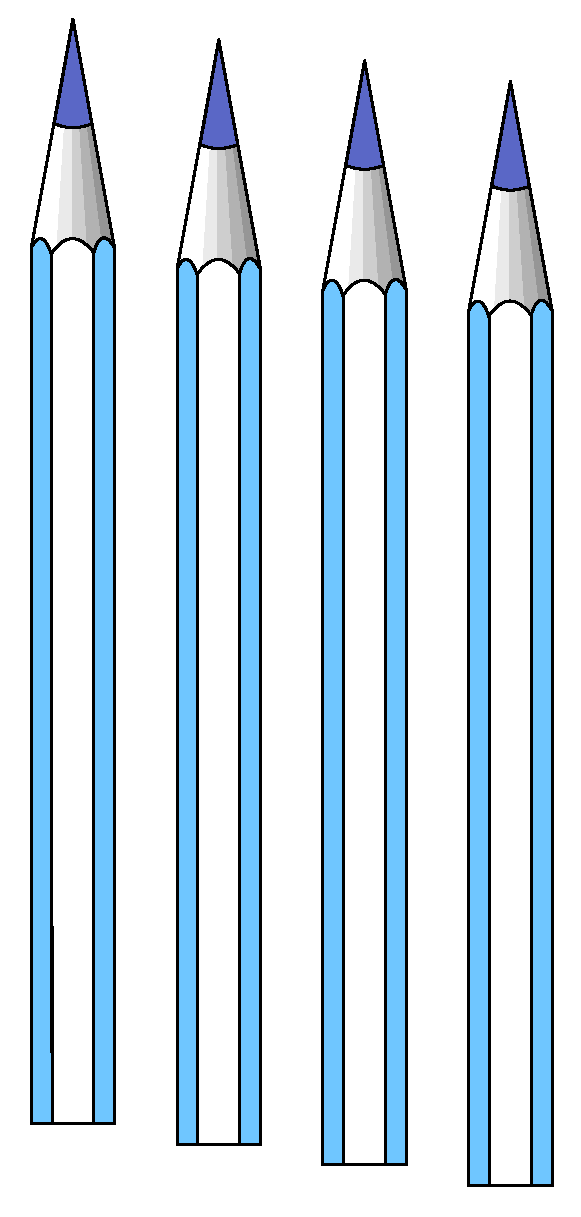
\includegraphics[angle=-90,width=0.9\textwidth]{pencils}}

  \vspace{\stretch{2}}

  %\htmladdnormallink{Wolfgang Dobler}{http://www.kis.uni-freiburg.de/~dobler/}
  %\&
  %\htmladdnormallink{Axel Brandenburg}{http://www.nordita.org/~brandenb/}

  \vspace{\stretch{1}}

  %\emph{$ $Date$ $,~ $ $Revision$ $}\\
  \today\\
  \url{http://www.nordita.org/software/pencil-code/}\\
  \url{https://github.com/pencil-code/pencil-code}

  \vspace{\stretch{3}}

\end{center}

\end{titlepage}


\newpage
\mbox{}

% ====================================================================== %

\section{Startup and run-time parameters}
\label{S-all-parameters}

\subsection[Startup parameters for \File{start.in}]%
{List of startup parameters for \file{start.in}}
\label{S-all-init-params}

The following table lists all (at the time of writing, September 2002)
namelists used in \file{start.in}, with the corresponding parameters
and their default values (in square brackets).
Any variable referred to as a \dfn{flag} can be set to any nonzero value
to switch the corresponding feature on.
Not all parameters are used for a given scenario.
This list is not necessarily up to date; also, in many cases it can only
give an idea of the corresponding initial state; to get more insight and
the latest set of parameters, you need to look at the code.

The value $\varepsilon$ corresponds to 5 times the smallest number larger
than zero.
For single precision, this is typically about
$\varepsilon \approx 5\times1.2{\times}10^{-7} = 6{\times}10^{-7}$; for
double precision, $\varepsilon\approx10^{-15}$.

% ---------------------------------------------------------------------- %
\begin{longtable}{lp{0.6\textwidth}}
%\begin{tabular}{lp{0.6\textwidth}}
\toprule
  \multicolumn{1}{c}{\emph{Variable [default value]}}
               & \multicolumn{1}{c}{\emph{Meaning}} \\
\midrule
  \multicolumn{2}{c}{Namelist \name{init_pars}}\\
\midrule
  \var{cvsid} [\code{''}]
               & the \name{svn} identification string, which allows you to
                 keep track of the version of \file{start.in}.\\
  \var{ip} [$14$]
               & (anti-)verbosity level: \code{ip=1} produces lots of
                 diagnostic output, \code{ip=14} virtually none. \\
  \var{xyz0} [$(-\pi,-\pi,-\pi)$],\\
  \var{Lxyz} [$(2\pi,2\pi,2\pi)$],\\
  \var{lperi} [(\code{T},\code{T},\code{T})]
               & determine the geometry of the box. All three are vectors
                 of the form ($x$-comp., $y$-comp., $z$-comp.); \var{xyz0}
                 describes the left (lower) corner of the box, \var{Lxyz}
                 the box size.
                 \var{lperi} specifies whether a direction is considered
                 periodic (in which case the last point is omitted) or not.
                 In all cases, three ghost zones will be added. \\
  \var{lprocz_slowest} [\code{T}]
               & if set to \code{F}, the ordering of processor numbers is
                 changed, so the $z$ processors are now in the inner loop.
                 Since \var{nprocy}=4 is optimal (see Sect.~\ref{Bandwidth}),
                 you may want to put \var{lprocz_slowest}=T when
                 \code{nygrid}$>$\code{nzgrid}.\\
  \var{lwrite_ic} [\code{F}]
               & if set \code{T}, the initial data are written into the
                 file \file{VAR0}. This is generally useful, but doing this
                 all the time uses up plenty of disk space.\\
  \var{lnowrite} [\code{F}]
               & if set \code{T}, all initialization files are written,
                 including the param.nml file,
                 except \file{var.dat}. This option allows you to use old
                 file{var.dat} files, but updates all other initialization
                 files. This could be useful after having changed the code
                 and, in particular, when the \file{var.dat} files will be
                 overwritten by \file{remesh.csh}.\\
  \var{lwrite_aux} [\code{F}]
               & if set \code{T}, auxiliary variables (those calculated at
                 each step, but not evolved mathematically) to
                 \file{var.dat} after the evolved quantities. \\
  \var{lwrite_2d} [\code{F}]
               & if set \code{T}, only 2D-snapshots are written into VAR
                 files in the case of 2D-runs with $nygrid=1$ or
                 $nzgrid=1$.\\
  \var{lread_oldsnap} [\code{F}]
               & if set \code{T}, the old snapshot will be read in before
                 producing (overwriting) initial conditions. For example, if
                 you just want to add a perturbation to the magnetic field,
                 you'd give no initial condition for density and velocity
                 (so you keep the data from a hopefully relaxed run),
                 and just add whatever you need for the magnetic field.
                 In this connection you may want to \cmd{touch NOERASE},
                 so as not to erase the previous data.\\
  \var{lread_oldsnap_nomag} [\code{F}]
               & if set \code{T}, the old snapshot from a non-magnetic run
                 will be read in before producing (overwriting) initial
                 conditions. This allows one to let a hydrodynamic
                 run relax before adding a magnetic field. However,
                 for this to work one has to modify {\it manually}
                 \file{data/param.nml} by adding an entry for
                 \var{MAGNETIC_INIT_PARS} or \var{PSCALAR_INIT_PARS}.
                 In addition, for \code{idl} to read correctly after the
                 first restarted run, you must adjust the value of \var{mvar}
                 in \file{data/dim.dat} \\
  \var{lread_oldsnap_nopscalar} [\code{F}]
               & if set \code{T}, the old snapshot from a run without
                 passive scalar will be read in before producing
                 (overwriting) initial conditions. This allows one to
                 let a hydrodynamic run relax before adding a passive
                 scalar.\\
  \var{lshift_origin} [\code{F,F,F}]
               & if set \code{T} for any or some of the three directions,
                 the mesh is shifted by 1/2 meshpoint in that or those
                 directions so that the mesh goes through the origin.\\
  \var{unit_system} [\code{'cgs'}]
               & you can set this character string to \index{SI units}
                 \code{'SI'}, which means that you can give \index{Units}
                 physical dimensions in \index{SI units} SI units.
                 The default is \index{cgs units} cgs units.\\
  \var{unit_length} [\code{1}]
               & allows you to set the unit length. Suppose you want
                 the unit length to be $1\,{\rm kpc}$, then you would
                 say \code{unit_length='3e21'}. (Of course, politically
                 correct would be to say \code{unit_system='SI'} in
                 which case you say \code{unit_length='3e19'}.)\\
  \var{unit_velocity} [\code{1}]
               & Example: if you want km/s you say \code{unit_length='1e5'}.\\
  \var{unit_density} [\code{1}]
               & Example: if you want your unit density to be
                 $10^{-24}\,{\rm g}/{\rm cm}^3$ you say
                 \code{unit_density='1e-24'}.\\
  \var{unit_temperature} [\code{1}]
               & Example: \code{unit_temperature='1e6'} if you want
                 mega-Kelvin.\\
  \var{random_gen} [\code{system}]
               & \label{random-gen-init}
                 choose random number generator;
                 currently valid choices are
                 \begin{description}
                 \item[\code{'system'}] (your compiler's generator),
                 \item[\code{'min_std'}] (the `minimal standard' generator
                   \code{ran0()} from `Numerical Recipes'),
                 \item[\code{'nr_f90'}] (the Parker-Miller-Marsaglia
                   generator \code{ran()} from `Numerical Recipes for
                   F90').
                 \end{description} \\
  \var{bcx} [(\code{'p'}, \code{'p'}, \ldots)], \\
  \var{bcy} [(\code{'p'}, \code{'p'}, \ldots)], \\
  \var{bcz} [(\code{'p'}, \code{'p'}, \ldots)]
               & boundary conditions. See Sect.~\ref{boundconds} for a
                 discussion of where and how to set these. \\
  \var{pretend_lnTT} [\code{F}]
                & \index{pretend_lnTT}
                selects $\ln T$ as fundamental thermodynamic variable
                in the entropy module \\
                 \\
%
\midrule
  \multicolumn{2}{c}{Namelist \name{hydro_init_pars}} \\
\midrule
  \var{inituu} [\code{'zero'}]
               & initialization of velocity. Currently valid choices are
                 \begin{description}
                 \item[\code{`zero'}] ($\uv=0$ ),
                 \item[\code{`gaussian-noise'}] (random,
                   normally-distributed $u_x$,$u_z$),
                 \item[\code{`gaussian-noise-x'}] (random,
                   normally-distributed $u_x$),
                 \item[\code{`sound-wave'}] (sound wave in $x$ direction),
                 \item[\code{`shock-tube'}] (polytropic standing shock),
                 \item[\code{`bullets'}] (blob-like velocity perturbations),
                 \item[\code{`Alfven-circ-x'}] (circularly polarized
                   Alfven wave in x direction),
                 \item[\code{`const-ux'}] (constant x-velocity),
                 \item[\code{`const-uy'}] (constant y-velocity),
                 \item[\code{`tang-discont-z'}] (tangential discontinuity:
                   velocity is directed along $x$, jump is at $z=0$),
                 \item[\code{`Fourier-trunc'}] (truncated Fourier series),
                 \item[\code{`up-down'}] (flow upward in one spot,
                   downward in another; not solenoidal).
                 \end{description}
                 \\
  \var{ampluu} [$0.$]
               & amplitude for some types of initial velocities. \\
  \var{widthuu} [$0.1$]
               & width for some types of initial velocities. \\
  \var{urand} [$0.$]
               & additional random perturbation of $\uv$. If
                 \verb|urand>0|, the perturbation is additive,
                 $u_i \mapsto u_i + u_{\rm rand}{\cal U}_{[0.5,0.5]}$;
                 if \verb|urand<0|, it is multiplicative,
                 $u_i \mapsto u_i \times u_{\rm rand}{\cal U}_{[0.5,0.5]}$;
                 in both cases, ${\cal U}_{[0.5,0.5]}$ is a uniformly
                 distributed random variable on the interval $[-0.5,0.5]$.\\
  \var{uu_left} [$0.$], \\
  \var{uu_right} [$0.$]
               & needed for \code{inituu='shock-tube'}.\\
%
\midrule
  \multicolumn{2}{c}{Namelist \name{density_init_pars}} \\
\midrule
  \var{initlnrho} [\code{'zero'}]
               & initialization of density. Currently valid choices are
                 \begin{description}
                 \item[\code{`zero'}] ($\ln\rho=0$),
                 \item[\code{`isothermal'}] (isothermal stratification),
                 \item[\code{`polytropic\_simple'}] (polytropic stratification),
                 \item[\code{`hydrostatic-z-2'}] (hydrostatic vertical
                   stratification for isentropic atmosphere),
                 \item[\code{`xjump'}] (density jump in $x$ of width
                   \var{widthlnrho}),
                 \item[\code{`rho-jump-z'}] (density jump in $z$ of width
                   \var{widthlnrho}),
                 \item[\code{`piecew-poly'}] (piecewise polytropic vertical
                   stratification for solar convection),
                 \item[\code{`polytropic'}] (polytropic vertical
                   stratification),
                 \item[\code{`sound-wave'}] (sound wave),
                 \item[\code{`shock-tube'}] (polytropic standing shock),
                 \item[\code{`gaussian-noise'}] (Gaussian-distributed,
                   uncorrelated noise),
                 \item[\code{`gaussian-noise'}] (Gaussian-distributed,
                   uncorrelated noise in $x$, but uniform in $y$ and $z$),
                 \item[\code{`hydrostatic-r'}] (hydrostatic radial density
                   stratification for isentropic or isothermal sphere),
                 \item[\code{`sin-xy'}] (sine profile in $x$ and $y$),
                 \item[\code{`sin-xy-rho'}] (sine profile in $x$ and $y$, but
                   in $\rho$, not $\ln\rho$),
                 \item[\code{`linear'}] (linear profile in $\kv\cdot\xv$),
                 \item[\code{`planet'}] (planet solution; see \S\ref{S-planet}).
                 \end{description}
                 \\
  \var{gamma} [$5./3$]
               & adiabatic index $\gamma=c_p/c_v$. \\
  \var{cs0} [$1.$]
               & can be used to set the dimension of velocity;
                 larger values can be used to decrease stratification \\
  \var{rho0} [$1.$]
               & \label{cs0-rho0-init}%
                 reference values of sound speed and density,
                 i.\,e.~values at height \var{zref}. \\
  \var{ampllnrho} [$0.$], \\
  \var{widthlnrho} [$0.1$]
               & amplitude and width for some types of initial densities. \\
  \var{rho_left} [$1.$], \\
  \var{rho_right} [$1.$]
               & needed for \code{initlnrho='shock-tube'}. \\
  \var{cs2bot} [$1.$], \\
  \var{cs2top} [$1.$]
               & sound speed at bottom and top. Needed for some types of
                 stratification. \\
%
\midrule
  \multicolumn{2}{c}{Namelist \name{grav_init_pars}} \\
\midrule
  \var{zref} [$0.$]
               & \label{zref-init}%
                 reference height where in the initial stratification
                 $c_{\rm s}^2=c_{\rm s0}^2$ and $\ln\rho=\ln\rho_0$.\\
  \var{gravz} [$-1.$]
               & vertical gravity component $g_z$.\\
  \var{grav_profile} \\{}
    [\code{'const'}]
               & constant gravity $g_z = \texttt{gravz}$
                 (\code{grav_profile='const'}) gravity
                 or linear profile $g_z = \texttt{gravz}\cdot z$
                 (\code{grav_profile='linear'}, for accretion discs and
                 similar). \\
  \var{z1} [$0.$], \\
  \var{z2} [$1.$]
               & specific to the solar convection case
                 \code{initlnrho='piecew-poly'}.
                 The stable layer is $z_0 < z < z_1$, the unstable layer
                 $z_1 < z < z_2$, and the top (isothermal) layer is
                 $z_2 < z < z_{\rm top}$. \\
  \var{nu_epicycle} [$1.$]
               & vertical epicyclic frequency; for accretion
                 discs it should be equal to Omega, but not for
                 galactic discs; see Eq.~(\ref{disc-gravz-init}) in
                 Sect.~\ref{VerticalStratification}.\\
  \var{grav_amp} [$0.$], \var{grav_tilt} [$0.$]
               & specific to the tilted gravity case (amplitude and angle
                 wrt the vertical direction).\\
%
\midrule
  \multicolumn{2}{c}{Namelist \name{entropy_init_pars}} \\
\midrule
  \var{initss} [\code{'nothing'}]
               & initialization of entropy. Currently valid choices are
                 \begin{description}
                 \item[\code{`nothing'}] (leaves the initialization done
                   in the density module unchanged),
                 \item[\code{`zero'}] (put $s=0$ explicitly; this may
                   overwrite the initialization done in the density module),
                 \item[\code{`isothermal'}] (isothermal stratification,
                   $T=\const$),
                 \item[\code{`isobaric'}] (isobaric, $p=\const$),
                 \item[\code{`isentropic'}] (isentropic with superimposed
                   hot [or cool] bubble),
                 \item[\code{`linprof'}] (linear entropy profile in $z$),
                 \item[\code{`piecew-poly'}] (piecewise polytropic
                   stratification for convection),
                 \item[\code{`polytropic'}] (polytropic stratification,
                   polytropic exponent is \var{mpoly0}),
                 \item[\code{`blob'}] (puts a gaussian blob in entropy for
                   buoyancy experiments; see Ref.~\cite{BH01} for details)
                 \item[\code{`xjump'}] (jump in $x$ direction),
                 \item[\code{`hor-tube'}] (horizontal flux tube in entropy,
                   oriented in the $y$-direction).
                 \end{description}
                 \\
  \var{pertss} [\code{'zero'}]
               & additional perturbation to entropy. Currently valid
                 choices are
                 \begin{description}
                 \item[\code{'zero'}] (no perturbation)
                 \item[\code{'hexagonal'}] (hexagonal perturbation for
                   convection).
                 \end{description}
                 \\
  \var{ampl_ss} [$0.$], \\
  \var{widthss} [$2\varepsilon$]
               & amplitude and width for some types of initial entropy. \\
  \var{grads0} [$0.$]
               & initial entropy gradient for \code{initss=linprof}. \\
  \var{radius_ss} [$0.1$]
               & radius of bubble for \code{initss=isentropic}. \\
  \var{mpoly0} [$1.5$], \\
  \var{mpoly1} [$1.5$], \\
  \var{mpoly2} [$1.5$]
               & \label{mpoly012-init}%
                 specific to the solar convection case
                 \code{initss=piecew-poly}:
                 polytropic indices of unstable (\var{mpoly0}), stable
                 (\var{mpoly1}) and top layer (\var{mpoly2}).
                 If the flag \var{isothtop} is set, the
                 top layer is initialized to be isothermal, otherwise
                 thermal (plus hydrostatic) equilibrium is assumed for all
                 three layers, which results in a piecewise polytropic
                 stratification. \\
  \var{isothtop} [$0$]
               & flag for isothermal top layer for \code{initss=piecew-poly}. \\
  \var{khor_ss} [$1.$]
               & horizontal wave number for \code{pertss=hexagonal} \\
%
\midrule
  \multicolumn{2}{c}{Namelist \name{magnetic_init_pars}} \\
\midrule
  \var{initaa} [\code{'zero'}]
               & initialization of magnetic field (vector potential).
                 Currently valid choices are
                 \begin{description}
                 \item[\code{`Alfven-x'}] (Alfv\'en wave traveling in the
                   $x$-direction; this also sets the velocity),
                 \item[\code{`Alfven-z'}] (Alfv\'en wave traveling in the
                   $z$-direction; this also sets the velocity),
                 \item[\code{`Alfvenz-rot'}] (same as \code{`Alfven-z'}, but
                   with rotation),
                 \item[\code{`Alfven-circ-x'}] (circularly polarized
                   Alfven wave in x direction),
                 \item[\code{`Beltrami-x'}] ($x$-dependent Beltrami wave),
                 \item[\code{`Beltrami-y'}] ($y$-dependent Beltrami wave),
                 \item[\code{`Beltrami-z'}] ($z$-dependent Beltrami wave),
                 \item[\code{`Bz(x)'}] ($B_z\propto\cos(k x)$),
                 \item[\code{`crazy'}] (for testing purposes).
                 \item[\code{`diffrot'}] ([needs to be documented]),
                 \item[\code{`fluxrings'}] (two interlocked magnetic fluxrings;
                   see \S~\ref{fluxrings}),
                 \item[\code{`gaussian-noise'}] (white noise),
                 \item[\code{`halfcos-Bx'}] ([needs to be documented]),
                 \item[\code{`hor-tube'}] (horizontal flux tube in $\Bv$,
                   oriented in the $y$-direction).
                 \item[\code{`hor-fluxlayer'}] (horizontal flux layer),
                 \item[\code{`mag-support'}] ([needs to be documented]),
                 \item[\code{`mode'}] ([needs to be documented]),
                 \item[\code{`modeb'}] ([needs to be documented]),
                 \item[\code{`propto-ux'}] ([needs to be documented]),
                 \item[\code{`propto-uy'}] ([needs to be documented]),
                 \item[\code{`propto-uz'}] ([needs to be documented]),
                 \item[\code{`sinxsinz'}] ($\sin x \sin z$),
                 \item[\code{`uniform-Bx'}] (uniform field in $x$ direction),
                 \item[\code{`uniform-By'}] (uniform field in $y$ direction),
                 \item[\code{`uniform-Bz'}] (uniform field in $z$ direction),
                 \item[\code{`zero'}] (zero field),
                 \end{description}
                 \\
  \var{initaa2} [\code{'zero'}]
               & additional perturbation of magnetic field.
                 Currently valid choices are
                 \begin{description}
                 \item[\code{`zero'}] (zero perturbation),
                 \item[\code{`Beltrami-x'}] ($x$-dependent Beltrami wave),
                 \item[\code{`Beltrami-y'}] ($y$-dependent Beltrami wave),
                 \item[\code{`Beltrami-z'}] ($z$-dependent Beltrami wave).
                 \end{description}
                 \\
  \var{amplaa} [$0.$]
               & amplitude for some types of initial magnetic fields. \\
  \var{amplaa2} [$0.$]
               & amplitude for some types of magnetic field perturbation. \\
  \var[fring1,fring2]{fring\{1,2\}} [$0.$], \\
  \var[Iring1,Iring2]{Iring\{1,2\}} [$0.$], \\
  \var[Rring1,Rring2]{Rring\{1,2\}} [$1.$], \\
  \var[wr1,wr2]{wr\{1,2\}} [$0.3$]
               & flux, current, outer and inner radius of flux ring 1/2;
                 see Sect.~\ref{fluxrings}. \\
  \var{radius} [$0.1$]
               & used by some initial fields. \\
  \var{epsilonaa} [$10^{-2}$]
               & used by some initial fields. \\
  \var{widthaa} [$0.5$]
               & used by some initial fields. \\
  \var{z0aa} [$0.$]
               & used by some initial fields. \\
  \var{kx_aa} [$1.$], \\
  \var{ky_aa} [$1.$], \\
  \var{kz_aa} [$1.$]
               & wavenumbers used by some initial fields. \\
  \var{lpress_equil} [F]
               & flag for pressure equilibrium (can be used in connection
                 with all initial fields) \\
%
\midrule
  \multicolumn{2}{c}{Namelist \name{pscalar_init_pars}} \\
\midrule
  \var{initlncc} [\code{'zero'}]
               & initialization of passive scalar
                 (concentration per unit mass, $c$).
                 Currently valid choices (for $\ln c$) are
                 \begin{description}
                 \item[\code{`zero'}] ($\ln c=0.$),
                 \item[\code{`gaussian-noise'}] (white noise),
                 \item[\code{`wave-x'}] (wave in $x$ direction),
                 \item[\code{`wave-y'}] (wave in $y$ direction),
                 \item[\code{`wave-z'}] (wave in $z$ direction),
                 \item[\code{`tang-discont-z'}] (Kelvin-Helmholtz instability),
                 \item[\code{`hor-tube'}] (horizontal tube in concentration;
                  used as a marker for magnetic flux tubes).
                 \end{description}
                 \\
  \var{initlncc2} [\code{'zero'}]
               & additional perturbation of passive scalar concentration $c$.
                 Currently valid choices are
                 \begin{description}
                 \item[\code{`zero'}] ($\delta\ln c=0.$),
                 \item[\code{`wave-x'}] (add $x$-directed wave to $\ln c$).
                 \end{description}
                 \\
\var{ampllncc} [$0.1$]
               & amplitude for some types of initial concentration. \\
  \var{ampllncc2} [$0.$]
               & amplitude for some types of concentration perturbation. \\
  \var{kx_lncc} [$1.$], \\
  \var{ky_lncc} [$1.$], \\
  \var{kz_lncc} [$1.$]
               & wave numbers for some types of initial concentration. \\
%
\midrule
  \multicolumn{2}{c}{Namelist \name{shear_init_pars}} \\
\midrule
  \var{qshear} [$0.$]
               & \label{qshear-init}%
                 degree of shear for shearing-box simulations (the
                 shearing-periodic boundaries are the $x$-boundaries and
                 are sheared in the $y$-direction). The shear velocity
                 is ${\bf U}=-q\varOmega x\,{\hat{\bf y}}$. \\
\midrule
  \multicolumn{2}{c}{Namelist \name{particles_ads_init_pars}} \\
\midrule
  \var{init_ads_mol_frac} [$0.$]
               & initial adsorbed mole fraction\\
\midrule
  \multicolumn{2}{c}{Namelist \name{particles_surf_init_pars}} \\
\midrule
  \var{init_surf_mol_frac} [$0.$]
               & initial surface mole fraction\\
\midrule
  \multicolumn{2}{c}{Namelist \name{particles_chem_init_pars}} \\
\midrule
  \var{total_carbon_sites} [$1.08e-8$]
               & carbon sites per surface area [mol/cm]2\\
\midrule
  \multicolumn{2}{c}{Namelist \name{particles_stalker_init_pars}} \\
\midrule
  \var{dstalk} [$0.1$]
               & times between printout of stalker data\\
  \var{lstalk_xx} [F]
               & particles position\\
  \var{lstalk_vv} [F]
               & particles velocity\\
  \var{lstalk_uu} [F]
               & gas velocity at particles position\\
  \var{lstalk_guu} [F]
               & gas velocity gradient at particles position\\
  \var{lstalk_rho} [F]
               & gas density at particles position\\
  \var{lstalk_grho} [F]
               & gas density gradient at particles position\\
  \var{lstalk_ap} [F]
               & particles diameter\\
  \var{lstalk_bb} [T]
               & magnetic field at particles position\\
  \var{lstalk_relvel} [F]
               &  particles relative velocity to gas\\
\bottomrule
%\end{tabular}
\end{longtable}
% ---------------------------------------------------------------------- %

\subsection[Runtime parameters for \File{run.in}]%
{List of runtime parameters for \file{run.in}}
\label{S-all-run-params}

The following table lists all (at the time of writing, September 2002)
namelists used in file \file{run.in}, with the corresponding
parameters and their default values (in square brackets).
Default values marked as [start] are taken from \file{start.in}.
Any variable referred to as a \dfn{flag} can be set to any nonzero value
to switch the corresponding feature on.
Not all parameters are used for a given scenario.
This list is not necessarily up to date; also, in many cases it can only
give an idea of the corresponding setup; to get more insight and
the latest set of parameters, you need to look at the code.

Once you have changed any of the \file{*.in} files, you may want to first
execute the command \code{pc_configtest} in order to test the correctness of
these configuration files, before you apply them in an active simulation run.


% ---------------------------------------------------------------------- %
\begin{longtable}{lp{0.6\textwidth}}
%\begin{tabular}{lp{0.6\textwidth}}
\toprule
  \multicolumn{1}{c}{\emph{Variable [default value]}}
               & \multicolumn{1}{c}{\emph{Meaning}} \\
\midrule
  \multicolumn{2}{c}{Namelist \name{run_pars}}\\
\midrule
  \var{cvsid} [\code{''}]
               & \name{svn} identification string, which allows you to
                 keep track of the version of \file{run.in}. \\
  \var{ip} [$14$]
               & (anti-)verbosity level: \code{ip=1} produces lots of
                 additional diagnostic output, \code{ip=14} virtually none. \\
  \var{nt} [$0$]
               & number of time steps to run. This number can be increased
                 or decreased during the run by \cmd{touch RELOAD}.\\
  \var{it1} [$10$]
               & write diagnostic output every \var{it1} time steps
                 (see Sect.~\ref{diagnostic-IO}). \\
  \var{it1d} [$it1$]
               & write averages every \var{it1d} time steps
                 (see Sect.~\ref{S-1d-averages}). \var{it1d} has to be
                 greater than or equal to \var{it1}.\\
  \var{cdt} [$0.4$]
               & Courant coefficient for advective time step; see
                 \S\ref{time-step}. \\
  \var{cdtv} [$0.08$]
               & Courant coefficient for diffusive time step; see
                 \S\ref{time-step}. \\
  \var{dt} [$0.$]
               & \label{dt-run}%
                 time step; if $\ne 0.$, this overwrites
                 the Courant time step. See \S\ref{time-step} for a
                 discussion of the latter. \\
  \var{dtmin} [$10^{-6}$]
               & abort if time step $\delta t < \delta t_{\rm min}$. \\
  \var{tmax} [$10^{33}$]
               & don't run time steps beyond this time. Useful if you want
                 to run for a given amount of time, but don't know the
                 necessary number of time steps.\\
  \var{isave} [$100$]
               & update current snapshot \file{var.dat} every \var{isave}
                 time steps. \\
  \var{itorder} [$3$]
               & order of time step (1 for Euler; 2 for 3nd-order, 3 for
                 3rd-order Runge--Kutta). \\
  \var{dsnap} [$100.$]
               & save permanent snapshot every \var{dsnap} time units to
                 files \file{VAR$N$}, where $N$ counts from $N=1$ upward.
                 (This information is stored in the file
                 \file[tsnap.dat]{data/tsnap.dat};
                 see the module \var{wsnaps.f90}, which in turn uses the
                 subroutines \var{out1} and \var{out2}). \\
  \var{dvid} [$100.$]
               & write two-dimensional sections for generation of videos
                 every \var{dvid} time units (not timesteps; see the
                 subroutines \var{out1} and \var{out2} in the code). \\
  \var{iwig} [$0$]
               & if $\ne 0$, apply a Nyquist filter (a filter eliminating
                 any signal at the Nyquist frequency, but affecting large
                 scales as little as possible) every \var{iwig} time steps to
                 logarithmic density (sometimes necessary with convection
                 simulations). \\
  \var{ix} [$-1$],
  \var{iy} [$-1$],
  \var{iz} [$-1$],
  \var{iz2} [$-1$]
               & position of slice planes for video files.
                 Any negative value of some of these variables will be
                 overwritten according to the value of
                 \var{slice_position}.
                 See \S~\ref{S-slices}) for details. \\
  \var{slice_position} ['p']
               & symbolic specification of slice position.
                 Currently valid choices are
                 \begin{description}
                 \item[\code{'p'}] (\emph{periphery} of the box)
                 \item[\code{'m'}] (\emph{middle} of the box)
                 \item[\code{'e'}] (\emph{equator} for half-sphere
                   calculations, i.\,e.~$x$, $y$ centered, $z$ bottom)
                 \end{description}
                 These settings are overridden by explicitly setting
                 \var{ix}, \var{iy}, \var{iz} or \var{iz2}.
                 See \S~\ref{S-slices}) for details. \\
  \var{zbot_slice} [value]
               & z position of slice xy-plane.
                 The value can be any float number inside the z domain.
                 These settings are overridden by explicitly setting
                 \var{ix}, \var{iy}, \var{iz} or \var{iz2}.
                 Saved as slice with the suffix \var{xy}.
                 See \S~\ref{S-slices}) for details. \\
   \var{ztop_slice} [value]
               & z position of slice xy-plane.
                 The value can be any float number inside the z domain.
                 These settings are overridden by explicitly setting
                 \var{ix}, \var{iy}, \var{iz} or \var{iz2}.
                 Saved as slice with the suffix \var{xy2}.
                 See \S~\ref{S-slices}) for details. \\
  \var{tavg} [$0$]
               & averaging time $\tau_{\rm avg}$ for time averages (if
                 $\ne 0$); at the same time, time interval for writing
                 time averages. See \S~\ref{S-time-averages} for details. \\
  \var{idx_tavg} [$(0,0,\ldots,0)$]
               & indices of variables to time-average.
                 See \S~\ref{S-time-averages} for details. \\
  \var{d2davg} [$100.$]
               & time interval for azimuthal and $z$-averages, i.e.~the
                 averages that produce 2d data.
                 See \S~\ref{S-phi-averages} for details. \\
  \var{ialive} [$0$]
               & if $\ne 0$, each processor writes the current time step
                 to \file{alive.info} every \var{ialive} time steps.
                 This provides the best test that the job is still alive.
                 (This can be used to find out which node has crashed
                 if there is a problem and the run is hanging.)\\
  \var{bcx} [(\code{'p'}, \code{'p'}, \ldots)], \\
  \var{bcy} [(\code{'p'}, \code{'p'}, \ldots)], \\
  \var{bcz} [(\code{'p'}, \code{'p'}, \ldots)]
               & boundary conditions. See Sect.~\ref{boundconds} for a
                 discussion of where and how to set these. \\
  \var{random_gen} [start]
               & see start parameters, p.~\pageref{random-gen-init} \\
  \var{lwrite_aux} [start]
               & if set \code{T}, auxiliary variables (those calculated at
                 each step, but not evolved mathematically) to
                 \file{var.dat} and \file{VAR} files after the evolved
                 quantities. \\
%
\midrule
  \multicolumn{2}{c}{Namelist \name{hydro_run_pars}} \\
\midrule
  \var{Omega} [$0.$]
               & magnitude of angular velocity for \name{Coriolis force}
                 (note: the centrifugal force is turned off by default,
                 unless \code{lcentrifugal_force=T} is set).\\
  \var{theta} [$0.$]
               & direction of angular velocity in degrees ($\theta=0$ for
                 $z$-direction, $\theta=90$ for the negative $x$-direction,
                 corresponding to a box located at the equator of a
                 rotating sphere.
                 Thus, e.g., $\theta=60$ corresponds to $30^\circ$ latitude.
                 (Note: prior to April 29, 2007, there was a minus sign in
                 the definition of $\theta$.)\\
  \var{ttransient} [$0.$]
               & initial time span for which to do something special
                 (transient).
                 Currently just used to smoothly switch on heating
                 [Should be in \name{run_pars}, rather than here]. \\
  \var{dampu} [$0.$], \\
  \var{tdamp} [$0.$], \\
  \var{ldamp_fade} [F]
               & damp motions during the initial time interval
                 $0<t<t_{\rm damp}$ with a damping term $-\var{dampu}(\uv)$.
                 If \var{ldamp_fade} is set, smoothly reduce damping to
                 zero over the second half of the time interval \var{tdamp}.
                 Initial velocity damping is useful for situations where
                 initial conditions are far from equilibrium. \\
  \var{dampuint} [$0.$],
               & weighting of damping external to spherical region
                 (see \var{wdamp}, $\var{damp}_u$ below). \\
  \var{dampuext} [$0.$],
               & weighting of damping in internal spherical region
                 (see \var{wdamp}, $\var{damp}_u$ below). \\
  \var{rdampint} [$0.$],
               & radius of internal damping region  \\
  \var{rdampext} [impossible],
               & radius of external damping region, used in place of
                 former variable \var{rdamp} \\
  \var{wdamp} [$0.2$],
               & permanently damp motions in $|\xv|<r_{\rm dampint}$
                 with damping term
                 $-\var{damp}_uint \,\uv\,\chi(r{-}r_{\rm dampint})$
                 or $|\xv|>r_{\rm dampext}$ with damping term
                 $-\var{damp}_uext \,\uv\,\chi(r{-}r_{\rm dampext})$,
                 where $\chi(\cdot)$ is a smooth profile of width
                 \var{wdamp}. \\
  \var{ampl_forc} [$0.$],
               & amplitude of the ux-forcing or uy-forcing on the vertical
                 boundaries that is of the form
                 $u\_x(t)=ampl\_forc*sin(k\_forc*x)*cos(w\_forc*t)$
                 [must be used in connection with bcx='g' or bcz=`g' and
                 force_lower_bound=`vel_time' or
                 force_upper_bound=`vel_time'] \\
  \var{k_forc} [$0.$],
               & corresponding horizontal wavenumber \\
  \var{w_forc} [$0.$]
               & corresponding frequency \\
%
\midrule
  \multicolumn{2}{c}{Namelist \name{density_run_pars}} \\
\midrule
  \var{cs0} [start], \\
  \var{rho0} [start], \\
  \var{gamma} [start]
               & \label{cs0-rho0-run}%
                 see start parameters, p.~\pageref{cs0-rho0-init} \\
  \var{cdiffrho} [$0.$]
               & Coefficient for mass diffusion (diffusion term will be
                 $c_{\rm diffrho}\,\delta x\, {\cs}_0$ . \\
  \var{cs2bot} [start], \\
  \var{cs2top} [start]
               & squared sound speed at bottom and top for boundary
                 condition \option{c2}. \\
  \var{lupw_lnrho} [.false.]
               & use 5th-order upwind derivative operator for the
               advection term $\uv\cdot\grad\ln\rho$ to avoid spurious
               Nyquist signal (`wiggles'); see \S\ref{S-upwind}. \\
%
\midrule
  \multicolumn{2}{c}{Namelist \name{entropy_run_pars}} \\
\midrule
  \var{hcond0} [$0.$], \\
  \var{hcond1} [start], \\
  \var{hcond2} [start]
               & specific to the solar convection case
                 \code{initss=piecew-poly}:
                 heat conductivities $K$ in the individual layers.
                 \var{hcond0} is the value $K_{\rm unst}$ in the
                 unstable layer, \var{hcond1} is the \emph{ratio}
                 $K_{\rm stab}/K_{\rm unst}$ for the stable
                 layer, and \var{hcond2} is the \emph{ratio}
                 $K_{\rm top}/K_{\rm unst}$ for the top layer.
                 The function $K(z)$ is not discontinuous, as the
                 transition between the different values is smoothed over
                 the width \var{widthss}.
                 If \var{hcond1} or \var{hcond2} are not set, they are
                 calculated according to the polytropic indices of the
                 initial profile, $K\propto m{+}1$. \\
  \var{iheatcond} [\code{'K-const'}]
               & select type of heat conduction.
                 Currently valid choices are
                 \begin{description}
                 \item[\code{`K-const'}]   (constant heat conductivity),
                 \item[\code{`K-profile'}] (vertical or radial profile),
                 \item[\code{`chi-const'}] (constant thermal diffusivity),
                 \item[\code{`magnetic'}]  (heat conduction by electrons
                   in magnetic field -- currently still experimental).
                 \end{description}
                 \\
  \var{lcalc_heatcond_constchi} [F]
               & flag for assuming thermal diffusivity
                 $\chi=K/(c_p\rho)=\const$, rather than $K=\const$
                 (which is the default).
                 \emph{This is currently only correct with
                 \file{noionization.f90}}.
                 Superseded by \var{iheatcond}. \\
  \var{chi} [$0.$]
               & value of $\chi$ when \code{lcalc_heatcond_constchi=T}. \\
  \var{widthss} [start]
               & width of transition region between layers.
                 See start parameters, p.~\pageref{mpoly012-init}. \\
  \var{isothtop} [start]
               & flag for isothermal top layer for solar convection case.
                 See start parameters, p.~\pageref{mpoly012-init}. \\
  \var{luminosity} [$0.$], \\
  \var{wheat} [$0.1$]
               & strength and width of heating region. \\
  \var{cooltype} [\code{'Temp'}]
               & type of cooling; \emph{currently only implemented for
                 spherical geometry}.
                 Currently valid choices are
                 \begin{description}
                 \item[\code{`Temp'},\code{`cs2'}] (cool temperature
                   toward $\cs^2=\var{cs2cool}$) with a cooling term
                   \[
                     -\mathcal{C} = -c_{\rm cool}
                                     \frac{\cs^2-{\cs^2}_{\rm cool}}
                                          {{\cs^2}_{\rm cool}}
                   \])
                 \item[\code{`Temp-rho'},\code{cs2-rho}]
                   (cool temperature toward $\cs^2=\var{cs2cool}$) with a
                   cooling term
                   \[
                     -\mathcal{C} = -c_{\rm cool}\,\rho\,
                                     \frac{\cs^2-{\cs^2}_{\rm cool}}
                                          {{\cs^2}_{\rm cool}}
                   \]
                   --- this avoids numerical instabilities in low-density
                   regions [currently, the cooling coefficient
                   $c_{\rm cool}\equiv$\var{cool} is not taken into account
                   when the time step is calculated])
                 \item[\code{`entropy'}] (cool entropy toward $0.$).
                 \end{description}
                 \\
  \var{cool} [$0.$], \\
  \var{wcool} [$0.1$]
               & strength $c_{\rm cool}$ and smoothing width of cooling
                 region. \\
  \var{rcool} [$1.$]
               & radius of cooling region: cool for
                 $|\xv| \ge \mbox{\var{rcool}}$.\\
  \var{Fbot} [start]
               & heat flux for bottom boundary condition \option{c1}.
                 For polytropic atmospheres, if \var{Fbot} is not set, it will
                 be calculated from the value of \var{hcond0} in \file{start.x},
                 provided the entropy boundary condition is set to \option{c1}. \\
  \var{chi_t} [$0.$]
               & entropy diffusion coefficient for diffusive term
                 $\partial s/\partial t = \ldots + \chi_{\rm t}\Laplace s$
                 in the entropy equation, that can represent some kind of
                 turbulent (sub-grid) mixing.
                 It is probably a bad idea to combine this with heat
                 conduction $\var{hcond0} \ne 0$. \\
  \var{lupw_ss} [.false.]
               & use 5th-order upwind derivative operator for the
                 advection term $\uv\cdot\grad s$ to avoid spurious Nyquist
                 signal (`wiggles'); see \S\ref{S-upwind}. \\
  \var{tauheat_buffer} [$0.$]
               & time scale for heating to target temperature
                 (=\var{TTheat_buffer}); zero disables the buffer zone. \\
  \var{zheat_buffer} [$0.$]
               & $z$ coordinate of the thermal buffer zone. Buffering
                 is active in $|z|>$\var{TTheat_buffer}. \\
  \var{dheat_buffer1} [$0.$]
               & Inverse thickness of transition to buffered layer.\\
  \var{TTheat_buffer} [$0.$]
               & target temperature in thermal buffer zone ($z$ direction only). \\
  \var{lhcond_global} [F]
               & flag for calculating the heat conductivity $K$ (and also
                 $\grad \log K$) globally using the global arrays facility.
                 Only valid when \var{iheatcond}=\code{`K-profile'}.\\
%
\midrule
  \multicolumn{2}{c}{Namelist \name{magnetic_run_pars}} \\
\midrule
  \var{B_ext} [$(0.,0.,0.)$]
               & uniform background magnetic field (for fully periodic
                 boundary conditions, uniform fields need to be explicitly
                 added, since otherwise the vector potential $\Av$ has a
                 linear $\xv$-dependence which is incompatible with
                 periodicity). \\
  \var{lignore_Bext_in_b2} [F]
               & add uniform background magnetic field when \\
  or \var{luse_Bext_in_b2} [T]
               & computing $\bv^2$ pencils\\
  \var{eta} [$0.$]
               & magnetic diffusivity $\eta=1/(\mu_0\sigma)$, where
                 $\sigma$ is the electric conductivity. \\
  \var{height_eta} [$0.$], \\
  \var{eta_out} [$0.$]
               & used to add extra diffusivity in a halo region. \\
  \var{eta_int} [$0.$]
               & used to add extra diffusivity inside sphere of
                 radius \var{r_int}. \\
  \var{eta_ext} [$0.$]
               & used to add extra diffusivity outside sphere of
                 radius \var{r_ext}. \\
  \var{kinflow} [\code{''}]
               & set type of flow fixed with \option{nohydro}. Currently
                 the only recognized value is \code{'ABC'} for an $ABC$
                 flow; all other values lead to $\uv=\zerovect$. \\
  \var{kx} [$1.$], \\
  \var{ky} [$1.$], \\
  \var{kz} [$1.$]
               & wave numbers for $ABC$ flow. \\
  \var{ABC_A} [$1.$], \\
  \var{ABC_B} [$1.$], \\
  \var{ABC_C} [$1.$]
               & amplitudes $A$, $B$ and $C$ for $ABC$ flow. \\
%
\midrule
  \multicolumn{2}{c}{Namelist \name{pscalar_run_pars}} \\
\midrule
  \var{pscalar_diff} [$0.$]
               & diffusion for passive scalar concentration $c$. \\
  \var{tensor_pscalar_diff} [$0.$]
               & coefficient for non-isotropic diffusion of passive scalar. \\
  \var{reinitialize_lncc} [F]
               & reinitialize the passive scalar to the value of cc\_const in start.in at next run\\
%
\midrule
  \multicolumn{2}{c}{Namelist \name{forcing_run_pars}} \\
\midrule
  \var{iforce} [$2$]
               & select form of forcing in the equation of motion;
                 currently valid choices are
                 \begin{description}
                 \item[\code{'zero'}] (no forcing),
                 \item[\code{'irrotational'}] (irrotational forcing),
                 \item[\code{'helical'}] (helical forcing),
                 \item[\code{'fountain'}] (forcing of ``fountain flow'';
                   see Ref.~\cite{BMS95}),
                 \item[\code{'horizontal-shear'}] (forcing localized
                   horizontal sinusoidal shear).
                 \item[\code{'variable_gravz'}] (time-dependent vertical
                   gravity for forcing internal waves),
                 \end{description}
                 \\
  \var{iforce2} [$0$]
               & select form of additional forcing in the equation of
                 motion; valid choices are as for \var{iforce}. \\
  \var{force} [$0.$]
               & amplitude of forcing. \\
  \var{relhel} [$1.$]
               & helicity of forcing. The parameter \var{relhel} corresponds
                 to $\sigma$ introduced in Sect.~\ref{SRandomForcingFunction}.
                 ($\sigma=\pm1$ corresponds to maximum helicity
                 of either sign). \\
  \var{height_ff} [$0.$]
               & multiply forcing by $z$-dependent profile of width
               \var{height_ff} (if $\ne 0$) . \\
  \var{r_ff} [$0.$]
               & if $\ne 0$, multiply forcing by spherical cutoff profile
                 (of radius \var{r_ff}) and flip signs of helicity at
                 equatorial plane. \\
  \var{width_ff} [$0.5$]
               & width of vertical and radial profiles for modifying
                 forcing. \\
  \var{kfountain} [$5$]
               & horizontal wavenumber of the fountain flow. \\
  \var{fountain} [$1.$]
               & amplitude of the fountain flow. \\
  \var{omega_ff} [$1.$]
               & frequency of the cos or sin forcing [e.g. cos(omega_ff*t)]. \\
  \var{ampl_ff} [$1.$]
               & amplitude of forcing in front of cos or sin [e.g.
                 ampl_ff*cos(omega_ff*t)]. \\
%
\midrule
  \multicolumn{2}{c}{Namelist \name{grav_run_pars}} \\
\midrule
  \var{zref} [start], \\
  \var{gravz} [start], \\
  \var{grav_profile} [start]
               & see p.~\pageref{zref-init}. \\
  \var{nu_epicycle} [start]
               & see Eq.~(\ref{disc-gravz-init}) in
                 Sect.~\ref{VerticalStratification}.\\
%
\midrule
  \multicolumn{2}{c}{Namelist \name{viscosity_run_pars}} \\
\midrule
  \var{nu} [$0.$]
               & kinematic viscosity. \\
  \var{nu_hyper2} [$0.$]
               & kinematic hyperviscosity (with $\nabla^4\uv$). \\
  \var{nu_hyper3} [$0.$]
               & kinematic hyperviscosity (with $\nabla^6\uv$). \\
  \var{zeta} [$0.$]
               & bulk viscosity. \\
  \var{ivisc} [\code{'nu-const'}]
               & select form of viscous term (see
                 \S\ref{S-Eqn-of-motion}); currently valid choices are
                 \begin{description}
                 \item[\code{'nu-const'}] -- viscous force for $\nu=\const$,
                   $\Fv_{\rm visc}=\nu(\Laplace\uv+{\textstyle{1\over3}}\grad\Div\uv
                    + 2\mathsf{S}\cdot\grad\ln\rho)$
                 \item[\code{'rho_nu-const'}] -- viscous force for
                   $\mu\equiv\rho\nu=\const$,
                   $\Fv_{\rm visc}=(\mu/\rho)(\Laplace\uv+{\textstyle{1\over3}}\grad\Div\uv)$.
                   With this option, the input parameter \var{nu} actually
                   sets the value of $\mu/\rho_0$
                   (\var{rho0}=$\rho_0$ is another input parameter, see
                   pp.~\pageref{cs0-rho0-init} and \pageref{cs0-rho0-run})
                 \item[\code{'simplified'}] -- simplified viscous force
                   $\Fv_{\rm visc}=\nu\Laplace\uv$
                 \end{description}
                 \\
%
\midrule
  \multicolumn{2}{c}{Namelist \name{shear_run_pars}} \\
\midrule
  \var{qshear} [start]
               & See p.~\pageref{qshear-init}. \\
\midrule
  \multicolumn{2}{c}{Namelist \name{particles_run_pars}} \\
\midrule
  \var{ldragforce_dust_par} [F]
               & dragforce on particles \\
  \var{ldragforce_gas_par} [F]
               & particle-gas friction force \\
  \var{ldraglaw_steadystate} [F]
               & particle forces only with $\frac{1}{\tau}\Delta v$ \\
  \var{lpscalar_sink} [F]
               & particles consume passive scalar \\
  \var{pscalar_sink_rate} [0]
               & volumetric pscalar consumption rate \\
  \var{lbubble} [F]
               & addition of the virtual mass term \\
\midrule
  \multicolumn{2}{c}{Namelist \name{particles_ads_run_pars}} \\
\midrule
  \var{placeholder} [start]
               & placeholder \\
\midrule
  \multicolumn{2}{c}{Namelist \name{particles_surf_run_pars}} \\
\midrule
  \var{lspecies_transfer [T]}
               & Species transfer from solid to fluid phase \\
\midrule
  \multicolumn{2}{c}{Namelist \name{particles_chem_run_pars}} \\
\midrule
  \var{lthiele [T]}
               & Modeling of particle porosity by application of Thiele modulus \\
\bottomrule
\end{longtable}
% ---------------------------------------------------------------------- %

\subsection[Parameters for \File{print.in}]%
{List of parameters for \file{print.in}}
\label{S-print.in-params}

The following table lists all possible inputs to the file \file{print.in}
that are documented.

% ---------------------------------------------------------------------- %
%% $Id$
%% This file was automatically generated by Pencil::DocExtractor,
%% so think twice before you modify it.
%%
%% Source files:
%%   cdata.f90
%%   hydro.f90
%%   density.f90
%%   entropy.f90
%%   magnetic.f90
%%   pscalar.f90
%%   testfield_compress_z.f90
%%   temperature_idealgas.f90
%%   testfield_x.f90
%%   testflow_z.f90
%%   viscosity.f90
%%   thermal_energy.f90
%%   shear.f90
%%   testfield_axisym.f90
%%   polymer.f90
%%   lorenz_gauge.f90
%%   testfield_z.f90
%%   nosolid_cells.f90
%%   chemistry.f90
%%   shock.f90
%%   noentropy.f90
%%   solid_cells.f90
%%   testfield_axisym2.f90
%%   testfield_nonlin_z.f90
%%   nolorenz_gauge.f90
%%   magnetic_axisym.f90
%%   testscalar.f90
%%   testfield_meri.f90

% ---------------------------------------------------------------- %
\begin{longtable}{lp{0.7\textwidth}}
\toprule
  \multicolumn{1}{c}{\emph{Variable}} & {\emph{Meaning}} \\
\midrule
  \multicolumn{2}{c}{Module \file{cdata.f90}} \\
\midrule
  \var{it}        & number of time step
                    \quad(since beginning of job only) \\
  \var{t}         & time $t$ \quad(since start.csh) \\
  \var{dt}        & time step $\delta t$ \\
  \var{walltime}  & wall clock time since start of
                    run.x, in seconds \\
  \var{Rmesh}     & $R_{\rm mesh}$ \\
  \var{Rmesh3}    & $R_{\rm mesh}^{(3)}$ \\
  \var{maxadvec}  & maxadvec \\
\midrule
  \multicolumn{2}{c}{Module \file{hydro.f90}} \\
\midrule
  \var{u2tm}      & $\left<\uv(t)\cdot\int_0^t\uv(t')
                    dt'\right>$ \\
  \var{uotm}      & $\left<\uv(t)\cdot\int_0^t\omv(t')
                    dt'\right>$ \\
  \var{outm}      & $\left<\omv(t)\cdot\int_0^t\uv(t')
                    dt'\right>$ \\
  \var{u2m}       & $\left<\uv^2\right>$ \\
  \var{uxpt}      & $u_x(x_1,y_1,z_1,t)$ \\
  \var{uypt}      & $u_x(x_1,y_1,z_1,t)$ \\
  \var{uzpt}      & $u_x(x_1,y_1,z_1,t)$ \\
  \var{uxp2}      & $u_x(x_2,y_2,z_2,t)$ \\
  \var{uyp2}      & $u_x(x_2,y_2,z_2,t)$ \\
  \var{uzp2}      & $u_x(x_2,y_2,z_2,t)$ \\
  \var{urms}      & $\left<\uv^2\right>^{1/2}$ \\
  \var{umax}      & $\max(|\uv|)$ \\
  \var{uzrms}     & $\left<u_z^2\right>^{1/2}$ \\
  \var{uxmin}     & $\min(|u_x|)$ \\
  \var{uymin}     & $\min(|u_y|)$ \\
  \var{uzmin}     & $\min(|u_z|)$ \\
  \var{uxmax}     & $\max(|u_x|)$ \\
  \var{uymax}     & $\max(|u_y|)$ \\
  \var{uzmax}     & $\max(|u_z|)$ \\
  \var{uxm}       & $\left<u_x\right>$ \\
  \var{uym}       & $\left<u_y\right>$ \\
  \var{uzm}       & $\left<u_z\right>$ \\
  \var{ux2m}      & $\left<u_x^2\right>$ \\
  \var{uy2m}      & $\left<u_y^2\right>$ \\
  \var{uz2m}      & $\left<u_z^2\right>$ \\
  \var{ux2ccm}    & $\left<u_x^2\cos^2kz\right>$ \\
  \var{ux2ssm}    & $\left<u_x^2\sin^2kz\right>$ \\
  \var{uy2ccm}    & $\left<u_y^2\cos^2kz\right>$ \\
  \var{uy2ssm}    & $\left<u_y^2\sin^2kz\right>$ \\
  \var{ux2mx}     & $\left<u_x^2\right>_{yz}$ \\
  \var{uy2mx}     & $\left<u_y^2\right>_{yz}$ \\
  \var{uz2mx}     & $\left<u_z^2\right>_{yz}$ \\
  \var{ox2mx}     & $\left<\omega_x^2\right>_{yz}$ \\
  \var{oy2mx}     & $\left<\omega_y^2\right>_{yz}$ \\
  \var{oz2mx}     & $\left<\omega_z^2\right>_{yz}$ \\
  \var{uxuycsm}   & $\left<u_xu_y\cos kz\sin kz\right>$ \\
  \var{ux2mz}     & $\left<u_x^2\right>_{xy}$ \\
  \var{uy2mz}     & $\left<u_y^2\right>_{xy}$ \\
  \var{uz2mz}     & $\left<u_z^2\right>_{xy}$ \\
  \var{rux2mz}    & $\left<\varrho u_x^2\right>_{xy}$ \\
  \var{ruy2mz}    & $\left<\varrho u_y^2\right>_{xy}$ \\
  \var{ruz2mz}    & $\left<\varrho u_z^2\right>_{xy}$ \\
  \var{uxuym}     & $\left<u_x u_y\right>$ \\
  \var{uxuzm}     & $\left<u_x u_z\right>$ \\
  \var{uyuzm}     & $\left<u_y u_z\right>$ \\
  \var{uxuymz}    & $\left<u_x u_y\right>_{xy}$ \\
  \var{uxuzmz}    & $\left<u_x u_z\right>_{xy}$ \\
  \var{uyuzmz}    & $\left<u_y u_z\right>_{xy}$ \\
  \var{oxuxxmz}   & $\left<\omega_x u_{x,x}\right>_{xy}$ \\
  \var{oyuxymz}   & $\left<\omega_y u_{x,y}\right>_{xy}$ \\
  \var{oxuyxmz}   & $\left<\omega_x u_{y,x}\right>_{xy}$ \\
  \var{oyuyymz}   & $\left<\omega_y u_{y,y}\right>_{xy}$ \\
  \var{oxuzxmz}   & $\left<\omega_x u_{z,x}\right>_{xy}$ \\
  \var{oyuzymz}   & $\left<\omega_y u_{z,y}\right>_{xy}$ \\
  \var{uxmz}      & $\left< u_x \right>_{x,y}$
                    \quad(horiz. averaged $x$
                    velocity) \\
  \var{divumz}    & $\left< {\rm div}\uv \right>_{xy}$ \\
  \var{uzdivumz}  & $\left< u_z{\rm div}\uv \right>_{xy}$ \\
  \var{oxmz}      & $\left< \omega_x \right>_{xy}$ \\
  \var{oymz}      & $\left< \omega_y \right>_{xy}$ \\
  \var{ozmz}      & $\left< \omega_z \right>_{xy}$ \\
  \var{umx}       & $\left< u_x \right>$ \\
  \var{umy}       & $\left< u_y \right>$ \\
  \var{umz}       & $\left< u_z \right>$ \\
  \var{uxmy}      & $\left< u_x \right>_{y}$ \\
  \var{uymy}      & $\left< u_y \right>_{y}$ \\
  \var{uzmy}      & $\left< u_z \right>_{y}$ \\
  \var{u2mz}      & $\left< \Uv^2 \right>_{xy}$ \\
  \var{o2mz}      & $\left< \Wv^2 \right>_{xy}$ \\
  \var{curlru2mz} & $\left<(\nabla\times\varrho\Uv)^2 \right>_{xy}$ \\
  \var{divru2mz}  & $\left<(\nabla\cdot\varrho\uv)^2\right>_{xy}$ \\
  \var{divu2mz}   & $\left<(\nabla\cdot\uv)^2\right>_{xy}$ \\
  \var{omumz}     & $\left<\left<\Wv\right>_{xy}
                    \cdot\left<\Uv\right>_{xy}
                    \right>$ \quad($xy$-averaged
                    mean cross helicity production) \\
  \var{umamz}     & $\left<\left<\uv\right>_{xy}\cdot\left<\Av\right>_{xy}\right>$ \\
  \var{umbmz}     & $\left<\left<\Uv\right>_{xy}
                    \cdot\left<\Bv\right>_{xy}
                    \right>$ \quad($xy$-averaged
                    mean cross helicity production) \\
  \var{umxbmz}    & $\left<\left<\Uv\right>_{xy}
                    \times\left<\Bv\right>_{xy}
                    \right>_z$ \quad($xy$-averaged
                    mean emf) \\
  \var{uxmxy}     & $\left< u_x \right>_{z}$ \\
  \var{uymxy}     & $\left< u_y \right>_{z}$ \\
  \var{uzmxy}     & $\left< u_z \right>_{z}$ \\
  \var{oxmxy}     & $\left< \omega_x \right>_{z}$ \\
  \var{oymxy}     & $\left< \omega_y \right>_{z}$ \\
  \var{ozmxy}     & $\left< \omega_z \right>_{z}$ \\
  \var{pvzmxy}    & $\left< (\omega_z + 2\Omega)/\varrho \right>_{z}$
                    \quad(z component of potential vorticity) \\
  \var{ruxmxy}    & $\left< \rho u_x \right>_{z}$ \\
  \var{ruymxy}    & $\left< \rho u_y \right>_{z}$ \\
  \var{ruzmxy}    & $\left< \rho u_z \right>_{z}$ \\
  \var{ux2mxy}    & $\left< u_x^2 \right>_{z}$ \\
  \var{uy2mxy}    & $\left< u_y^2 \right>_{z}$ \\
  \var{uz2mxy}    & $\left< u_z^2 \right>_{z}$ \\
  \var{rux2mxy}   & $\left< \rho u_x^2 \right>_{z}$ \\
  \var{ruy2mxy}   & $\left< \rho u_y^2 \right>_{z}$ \\
  \var{ruz2mxy}   & $\left< \rho u_z^2 \right>_{z}$ \\
  \var{ruxuymxy}  & $\left< \rho u_x u_y \right>_{z}$ \\
  \var{ruxuzmxy}  & $\left< \rho u_x u_z \right>_{z}$ \\
  \var{ruyuzmxy}  & $\left< \rho u_y u_z \right>_{z}$ \\
  \var{rux2m}     & $\left<\rho u_x^2\right>$ \\
  \var{ruy2m}     & $\left<\rho u_y^2\right>$ \\
  \var{ruz2m}     & $\left<\rho u_z^2\right>$ \\
  \var{uxmxz}     & $\left< u_x \right>_{y}$ \\
  \var{uymxz}     & $\left< u_y \right>_{y}$ \\
  \var{uzmxz}     & $\left< u_z \right>_{y}$ \\
  \var{ux2mxz}    & $\left< u_x^2 \right>_{y}$ \\
  \var{uy2mxz}    & $\left< u_y^2 \right>_{y}$ \\
  \var{uz2mxz}    & $\left< u_z^2 \right>_{y}$ \\
  \var{uxuymxz}   & $\left< u_x u_y \right>_{y}$ \\
  \var{uxuzmxz}   & $\left< u_x u_z \right>_{y}$ \\
  \var{uyuzmxz}   & $\left< u_y u_z \right>_{y}$ \\
  \var{uxmx}      & $\left< u_x \right>_{yz}$ \\
  \var{uymx}      & $\left< u_y \right>_{yz}$ \\
  \var{uzmx}      & $\left< u_z \right>_{yz}$ \\
  \var{divum}     & $\left<{\rm div}\uv)\right>$ \\
  \var{divu2m}    & $\left<({\rm div}\uv)^2\right>$ \\
  \var{u3u21m}    & $\left<u_3 u_{2,1}\right>$ \\
  \var{u1u32m}    & $\left<u_1 u_{3,2}\right>$ \\
  \var{u2u13m}    & $\left<u_2 u_{1,3}\right>$ \\
  \var{u2u31m}    & $\left<u_2 u_{3,1}\right>$ \\
  \var{u3u12m}    & $\left<u_3 u_{1,2}\right>$ \\
  \var{u1u23m}    & $\left<u_1 u_{2,3}\right>$ \\
  \var{ruxm}      & $\left<\varrho u_x\right>$
                    \quad(mean $x$-momentum density) \\
  \var{ruym}      & $\left<\varrho u_y\right>$
                    \quad(mean $y$-momentum density) \\
  \var{ruzm}      & $\left<\varrho u_z\right>$
                    \quad(mean $z$-momentum density) \\
  \var{ruxtot}    & $\left<\rho |u|\right>$
                    \quad(mean absolute $x$-momentum density) \\
  \var{rumax}     & $\max(\varrho |\uv|)$
                    \quad(maximum modulus of momentum) \\
  \var{ruxuym}    & $\left<\varrho u_x u_y\right>$
                    \quad(mean Reynolds stress) \\
  \var{ruxuzm}    & $\left<\varrho u_x u_z\right>$
                    \quad(mean Reynolds stress) \\
  \var{ruyuzm}    & $\left<\varrho u_y u_z\right>$
                    \quad(mean Reynolds stress) \\
  \var{rlxm}      & $\left< \rho y u_z - z u_y \right>$ \\
  \var{rlym}      & $\left< \rho z u_x - x u_z \right>$ \\
  \var{rlzm}      & $\left< \rho x u_y - y u_x \right>$ \\
  \var{rlx2m}     & $\left<(\rho y u_z-z u_y)^2\right>$ \\
  \var{rly2m}     & $\left<(\rho z u_x-x u_z)^2\right>$ \\
  \var{rlz2m}     & $\left<(\rho x u_y-y u_x)^2\right>$ \\
  \var{tot_ang_mom} & Total angular momentum in spherical
                    coordinates about the axis. \\
  \var{dtu}       & $\delta t/[c_{\delta t}\,\delta x
                    /\max|\mathbf{u}|]$
                    \quad(time step relative to
                    advective time step;
                    see \S~\ref{time-step}) \\
  \var{oum}       & $\left<\boldsymbol{\omega}
                    \cdot\uv\right>$ \\
  \var{fum}       & $\left<\fv\cdot\uv\right>$ \\
  \var{odel2um}   & $\left<\boldsymbol{\omega}\nabla^2\uv\right>$ \\
  \var{o2m}       & $\left<\boldsymbol{\omega}^2\right>
                    \equiv \left<(\curl\uv)^2\right>$ \\
  \var{orms}      & $\left<\boldsymbol{\omega}^2
                    \right>^{1/2}$ \\
  \var{omax}      & $\max(|\boldsymbol{\omega}|)$ \\
  \var{ox2m}      & $\left<\omega_x^2\right>$ \\
  \var{oy2m}      & $\left<\omega_y^2\right>$ \\
  \var{oz2m}      & $\left<\omega_z^2\right>$ \\
  \var{oxoym}     & $\left<\omega_x\omega_y\right>$ \\
  \var{oxozm}     & $\left<\omega_x\omega_z\right>$ \\
  \var{oyozm}     & $\left<\omega_y\omega_z\right>$ \\
  \var{pvzm}      & $\left<\omega_z + 2\Omega/\varrho\right>$
                    \quad(z component of potential vorticity) \\
  \var{oumphi}    & $\left<\omv\cdot\uv\right>_\varphi$ \\
  \var{oumx}      & $\left<\boldsymbol{\omega}
                    \cdot\uv\right>_{yz}$ \\
  \var{oumy}      & $\left<\boldsymbol{\omega}
                    \cdot\uv\right>_{xz}$ \\
  \var{oumz}      & $\left<\boldsymbol{\omega}
                    \cdot\uv\right>_{xy}$ \\
  \var{oumxy}     & $\left<\boldsymbol{\omega}
                    \cdot\uv\right>_{z}$ \\
  \var{oumxz}     & $\left<\boldsymbol{\omega}
                    \cdot\uv\right>_{y}$ \\
  \var{Marms}     & $\left<\uv^2/\cs^2\right>$
                    \quad(rms Mach number) \\
  \var{Mamax}     & $\max |\uv|/\cs$
                    \quad(maximum Mach number) \\
  \var{ekin}      & $\left<{1\over2}\varrho\uv^2\right>$ \\
  \var{ekintot}   & $\int_V{1\over2}\varrho\uv^2\, dV$ \\
  \var{fkinzmz}   & $\left<{1\over2}\varrho\uv^2 u_z\right>_{xy}$ \\
  \var{fkinxmxy}  & $\left<{1\over2}\varrho\uv^2 u_x\right>_{z}$ \\
  \var{uxglnrym}  & $\left<u_x\partial_y\ln\varrho\right>$ \\
  \var{uyglnrxm}  & $\left<u_y\partial_x\ln\varrho\right>$ \\
  \var{uzdivum}   & $\left<u_z\nabla\cdot\uv\right>$ \\
  \var{uxuydivum} & $\left<u_x u_y\nabla\cdot\uv\right>$ \\
  \var{divuHrms}  & $(\nabla_{\rm H}\cdot\uv_{\rm H})^{\rm rms}$ \\
  \var{uxxrms}    & $u_{x,x}^{\rm rms}$ \\
  \var{uyyrms}    & $u_{y,y}^{\rm rms}$ \\
  \var{uxzrms}    & $u_{x,z}^{\rm rms}$ \\
  \var{uyzrms}    & $u_{y,z}^{\rm rms}$ \\
  \var{uzyrms}    & $u_{z,y}^{\rm rms}$ \\
\midrule
  \multicolumn{2}{c}{Module \file{density.f90}} \\
\midrule
  \var{rhom}      & $\left<\varrho\right>$
                    \quad(mean density) \\
  \var{rhomin}    & $\min(\rho)$ \\
  \var{rhomax}    & $\max(\rho)$ \\
  \var{ugrhom}    & $\left<\uv\cdot\nabla\varrho\right>$ \\
  \var{rhomz}     & $\left<\varrho\right>_{xy}$ \\
  \var{totmass}   & $\int\varrho\,dV$ \\
  \var{mass}      & $\int\varrho\,dV$ \\
  \var{grhomax}   & $\max (|\nabla \varrho|)$ \\
\midrule
  \multicolumn{2}{c}{Module \file{entropy.f90}} \\
\midrule
  \var{dtc}       & $\delta t/[c_{\delta t}\,\delta_x
                    /\max c_{\rm s}]$
                    \quad(time step relative to
                    acoustic time step;
                    see \S~\ref{time-step}) \\
  \var{ethm}      & $\left<\varrho e\right>$
                    \quad(mean thermal
                    [=internal] energy) \\
  \var{ssm}       & $\left<s/c_p\right>$
                    \quad(mean entropy) \\
  \var{ss2m}      & $\left<(s/c_p)^2\right>$
                    \quad(mean squared entropy) \\
  \var{eem}       & $\left<e\right>$ \\
  \var{ppm}       & $\left<p\right>$ \\
  \var{csm}       & $\left<c_{\rm s}\right>$ \\
  \var{pdivum}    & $\left<p\nabla\uv\right>$ \\
  \var{fradbot}   & $\int F_{\rm bot}\cdot d\vec{S}$ \\
  \var{fradtop}   & $\int F_{\rm top}\cdot d\vec{S}$ \\
  \var{TTtop}     & $\int T_{\rm top} d\vec{S}$ \\
  \var{ethtot}    & $\int_V\varrho e\,dV$
                    \quad(total thermal
                    [=internal] energy) \\
  \var{dtchi}     & $\delta t / [c_{\delta t,{\rm v}}\,
                    \delta x^2/\chi_{\rm max}]$
                    \quad(time step relative to time
                    step based on heat conductivity;
                    see \S~\ref{time-step}) \\
  \var{yHm}       & mean hydrogen ionization \\
  \var{yHmax}     & max of hydrogen ionization \\
  \var{TTm}       & $\left<T\right>$ \\
  \var{TTmax}     & $T_{\max}$ \\
  \var{TTmin}     & $T_{\min}$ \\
  \var{ssmax}     & $s_{\max}$ \\
  \var{ssmin}     & $s_{\min}$ \\
  \var{gTrms}     & $(\nabla T)_{\rm rms}$ \\
  \var{gsrms}     & $(\nabla s)_{\rm rms}$ \\
  \var{gTxgsrms}  & $(\nabla T\times\nabla s)_{\rm rms}$ \\
  \var{fconvm}    & $\left<\varrho u_z T \right>$ \\
  \var{fconvz}    & $\left<\varrho u_z T \right>_{xy}$ \\
  \var{fconvxy}   & $\left<\varrho u_x T \right>_{z}$ \\
  \var{fconvyxy}  & $\left<\varrho u_y T \right>_{z}$ \\
  \var{fconvzxy}  & $\left<\varrho u_z T \right>_{z}$ \\
  \var{dcoolz}    & surface cooling flux \\
  \var{dcoolxy}   & surface cooling flux \\
  \var{fradz}     & $F_{\rm rad}$ \\
  \var{fradz_Kprof} & $F_{\rm rad}$ (from Kprof) \\
  \var{fradxy_Kprof} & $F_{\rm rad}$ ($xy$-averaged, from Kprof) \\
  \var{fradz_kramers} & $F_{\rm rad}$ (from Kramers'
                    opacity) \\
  \var{fradxy_kramers} & $F_{\rm rad}$ ($xy$-averaged,
                    from Kramers' opacity) \\
  \var{fturbz}    & $\left<\varrho T \chi_t \nabla_z
                    s\right>_{xy}$ \quad(turbulent
                    heat flux) \\
  \var{fturbxy}   & $\left<\varrho T \chi_t \nabla_x
                    s\right>_{z}$ \\
  \var{fturbrxy}  & $\left<\varrho T \chi_{ri} \nabla_i
                    s\right>_{z}$ \quad(radial part
                    of anisotropic turbulent heat flux) \\
  \var{fturbthxy} & $\left<\varrho T \chi_{\theta i}
                    \nabla_i s\right>_{z}$ \quad
                    (latitudinal part of anisotropic
                    turbulent heat flux) \\
  \var{TTmz}      & $\left< T \right>_{xy}$ \\
  \var{TT2mz}     & $\left< T^2 \right>_{xy}$ \\
  \var{uxTTmz}    & $\left< u_x T \right>_{xy}$ \\
  \var{uyTTmz}    & $\left< u_y T \right>_{xy}$ \\
  \var{uzTTmz}    & $\left< u_z T \right>_{xy}$ \\
  \var{uxTTmxy}   & $\left< u_x T \right>_{z}$ \\
  \var{uyTTmxy}   & $\left< u_y T \right>_{z}$ \\
  \var{uzTTmxy}   & $\left< u_z T \right>_{z}$ \\
  \var{ssmxy}     & $\left< s \right>_{z}$ \\
  \var{ssmxz}     & $\left< s \right>_{y}$ \\
  \var{ufpresm}   & $\left< -u/\rho\nabla p \right>$ \\
\midrule
  \multicolumn{2}{c}{Module \file{magnetic.f90}} \\
\midrule
  \var{ab_int}    & $\int\Av\cdot\Bv\;dV$ \\
  \var{jb_int}    & $\int\jv\cdot\Bv\;dV$ \\
  \var{b2tm}      & $\left<\bv(t)\cdot\int_0^t\bv(t')
                    dt'\right>$ \\
  \var{bjtm}      & $\left<\bv(t)\cdot\int_0^t\jv(t')
                    dt'\right>$ \\
  \var{jbtm}      & $\left<\jv(t)\cdot\int_0^t\bv(t')
                    dt'\right>$ \\
  \var{b2ruzm}    & $\left<\Bv^2\rho u_z\right>$ \\
  \var{b2uzm}     & $\left<\Bv^2u_z\right>$ \\
  \var{ubbzm}     & $\left<(\uv\cdot\Bv)B_z\right>$ \\
  \var{b1m}       & $\left<|\Bv|\right>$ \\
  \var{b2m}       & $\left<\Bv^2\right>$ \\
  \var{bm2}       & $\max(\Bv^2)$ \\
  \var{j2m}       & $\left<\jv^2\right>$ \\
  \var{jm2}       & $\max(\jv^2)$ \\
  \var{abm}       & $\left<\Av\cdot\Bv\right>$ \\
  \var{abumx}     & $\left<u_x\Av\cdot\Bv\right>$ \\
  \var{abumy}     & $\left<u_y\Av\cdot\Bv\right>$ \\
  \var{abumz}     & $\left<u_z\Av\cdot\Bv\right>$ \\
  \var{abmh}      & $\left<\Av\cdot\Bv\right>$ (temp) \\
  \var{abmn}      & $\left<\Av\cdot\Bv\right>$ (north) \\
  \var{abms}      & $\left<\Av\cdot\Bv\right>$ (south) \\
  \var{abrms}     & $\left<(\Av\cdot\Bv)^2\right>^{1/2}$ \\
  \var{jbrms}     & $\left<(\jv\cdot\Bv)^2\right>^{1/2}$ \\
  \var{ajm}       & $\left<\jv\cdot\Av\right>$ \\
  \var{jbm}       & $\left<\jv\cdot\Bv\right>$ \\
  \var{jbmh}      & $\left<\Jv\cdot\Bv\right>$ (temp) \\
  \var{jbmn}      & $\left<\Jv\cdot\Bv\right>$ (north) \\
  \var{jbms}      & $\left<\Jv\cdot\Bv\right>$ (south) \\
  \var{ubm}       & $\left<\uv\cdot\Bv\right>$ \\
  \var{dubrms}    & $\left<(\uv-\Bv)^2\right>^{1/2}$ \\
  \var{dobrms}    & $\left<(\boldsymbol{\omega}-\Bv)^2
                    \right>^{1/2}$ \\
  \var{uxbxm}     & $\left<u_xB_x\right>$ \\
  \var{uybym}     & $\left<u_yB_y\right>$ \\
  \var{uzbzm}     & $\left<u_zB_z\right>$ \\
  \var{cosubm}    & $\left<\Uv\cdot\Bv/(|\Uv|\,|\Bv|)
                    \right>$ \\
  \var{uam}       & $\left<\uv\cdot\Av\right>$ \\
  \var{ujm}       & $\left<\uv\cdot\Jv\right>$ \\
  \var{fbm}       & $\left<\fv\cdot\Bv\right>$ \\
  \var{fxbxm}     & $\left<f_x B_x\right>$ \\
  \var{epsM}      & $\left<\eta\mu_0\jv^2\right>$ \\
  \var{epsAD}     & $\left<\rho^{-1} t_{\rm AD}
                    (\vec{J}\times\vec{B})^2\right>$
                    (heating by ion-neutrals friction) \\
  \var{bxpt}      & $B_x(x_1,y_1,z_1,t)$ \\
  \var{bypt}      & $B_y(x_1,y_1,z_1,t)$ \\
  \var{bzpt}      & $B_z(x_1,y_1,z_1,t)$ \\
  \var{jxpt}      & $J_x(x_1,y_1,z_1,t)$ \\
  \var{jypt}      & $J_y(x_1,y_1,z_1,t)$ \\
  \var{jzpt}      & $J_z(x_1,y_1,z_1,t)$ \\
  \var{Expt}      & ${\cal E}_x(x_1,y_1,z_1,t)$ \\
  \var{Eypt}      & ${\cal E}_y(x_1,y_1,z_1,t)$ \\
  \var{Ezpt}      & ${\cal E}_z(x_1,y_1,z_1,t)$ \\
  \var{axpt}      & $A_x(x_1,y_1,z_1,t)$ \\
  \var{aypt}      & $A_y(x_1,y_1,z_1,t)$ \\
  \var{azpt}      & $A_z(x_1,y_1,z_1,t)$ \\
  \var{bxp2}      & $B_x(x_2,y_2,z_2,t)$ \\
  \var{byp2}      & $B_y(x_2,y_2,z_2,t)$ \\
  \var{bzp2}      & $B_z(x_2,y_2,z_2,t)$ \\
  \var{jxp2}      & $J_x(x_2,y_2,z_2,t)$ \\
  \var{jyp2}      & $J_y(x_2,y_2,z_2,t)$ \\
  \var{jzp2}      & $J_z(x_2,y_2,z_2,t)$ \\
  \var{Exp2}      & ${\cal E}_x(x_2,y_2,z_2,t)$ \\
  \var{Eyp2}      & ${\cal E}_y(x_2,y_2,z_2,t)$ \\
  \var{Ezp2}      & ${\cal E}_z(x_2,y_2,z_2,t)$ \\
  \var{axp2}      & $A_x(x_2,y_2,z_2,t)$ \\
  \var{ayp2}      & $A_y(x_2,y_2,z_2,t)$ \\
  \var{azp2}      & $A_z(x_2,y_2,z_2,t)$ \\
  \var{exabot}    & $\int\Ev\times\Av\,dS|_{\rm bot}$ \\
  \var{exatop}    & $\int\Ev\times\Av\,dS|_{\rm top}$ \\
  \var{emag}      & $\int_V{1\over2\mu_0}\Bv^2\, dV$ \\
  \var{brms}      & $\left<\Bv^2\right>^{1/2}$ \\
  \var{bmax}      & $\max(|\Bv|)$ \\
  \var{bxmin}     & $\min(|B_x|)$ \\
  \var{bymin}     & $\min(|B_y|)$ \\
  \var{bzmin}     & $\min(|B_z|)$ \\
  \var{bxmax}     & $\max(|B_x|)$ \\
  \var{bymax}     & $\max(|B_y|)$ \\
  \var{bzmax}     & $\max(|B_z|)$ \\
  \var{jrms}      & $\left<\jv^2\right>^{1/2}$ \\
  \var{hjrms}     & $\left<\jv^2\right>^{1/2}$ \\
  \var{jmax}      & $\max(|\jv|)$ \\
  \var{vArms}     & $\left<\Bv^2/\varrho\right>^{1/2}$ \\
  \var{vAmax}     & $\max(\Bv^2/\varrho)^{1/2}$ \\
  \var{dtb}       & $\delta t / [c_{\delta t}\,\delta x
                    /v_{\rm A,max}]$
                    \quad(time step relative to
                    Alfv{\'e}n time step;
                    see \S~\ref{time-step}) \\
  \var{dteta}     & $\delta t/[c_{\delta t,{\rm v}}\,
                    \delta x^2/\eta_{\rm max}]$
                    \quad(time step relative to
                    resistive time step;
                    see \S~\ref{time-step}) \\
  \var{a2m}       & $\left<\Av^2\right>$ \\
  \var{arms}      & $\left<\Av^2\right>^{1/2}$ \\
  \var{amax}      & $\max(|\Av|)$ \\
  \var{beta1m}    & $\left<\Bv^2/(2\mu_0 p)\right>$
                    \quad(mean inverse plasma beta) \\
  \var{beta1max}  & $\max[\Bv^2/(2\mu_0 p)]$
                    \quad(maximum inverse plasma beta) \\
  \var{bxm}       & $\left<\left<B\right>_{yz}^2\right>_x^{1/2}$ \\
  \var{bym}       & $\left<\left<B\right>_{zx}^2\right>_y^{1/2}$ \\
  \var{bzm}       & $\left<\left<B\right>_{xy}^2\right>_z^{1/2}$ \\
  \var{bxbym}     & $\left<B_x B_y\right>$ \\
  \var{bxbymx}    & $\left<B_x B_y\right>_{yz}$ \\
  \var{b2mz}      & $\left<\Bv^2\right>_{xy}$ \\
  \var{axmz}      & $\left<{\cal A}_x\right>_{xy}$ \\
  \var{aymz}      & $\left<{\cal A}_y\right>_{xy}$ \\
  \var{azmz}      & $\left<{\cal A}_z\right>_{xy}$ \\
  \var{abuxmz}    & $\left<(\Av \cdot \Bv) u_x \right>_{xy}$ \\
  \var{abuymz}    & $\left<(\Av \cdot \Bv) u_y \right>_{xy}$ \\
  \var{abuzmz}    & $\left<(\Av \cdot \Bv) u_z \right>_{xy}$ \\
  \var{uabxmz}    & $\left<(\uv \cdot \Av) B_x \right>_{xy}$ \\
  \var{uabymz}    & $\left<(\uv \cdot \Av) B_y \right>_{xy}$ \\
  \var{uabzmz}    & $\left<(\uv \cdot \Av) B_z \right>_{xy}$ \\
  \var{bbxmz}     & $\left<{\cal B}'_x\right>_{xy}$ \\
  \var{bbymz}     & $\left<{\cal B}'_y\right>_{xy}$ \\
  \var{bbzmz}     & $\left<{\cal B}'_z\right>_{xy}$ \\
  \var{bxmz}      & $\left<{\cal B}_x\right>_{xy}$ \\
  \var{bymz}      & $\left<{\cal B}_y\right>_{xy}$ \\
  \var{bzmz}      & $\left<{\cal B}_z\right>_{xy}$ \\
  \var{jxmz}      & $\left<{\cal J}_x\right>_{xy}$ \\
  \var{jymz}      & $\left<{\cal J}_y\right>_{xy}$ \\
  \var{jzmz}      & $\left<{\cal J}_z\right>_{xy}$ \\
  \var{Exmz}      & $\left<{\cal E}_x\right>_{xy}$ \\
  \var{Eymz}      & $\left<{\cal E}_y\right>_{xy}$ \\
  \var{Ezmz}      & $\left<{\cal E}_z\right>_{xy}$ \\
  \var{bmx}       & $\left<\left<\Bv\right>_{yz}^2
                    \right>^{1/2}$
                    \quad(energy of $yz$-averaged
                    mean field) \\
  \var{bmy}       & $\left<\left<\Bv\right>_{xz}^2
                    \right>^{1/2}$
                    \quad(energy of $xz$-averaged
                    mean field) \\
  \var{bmz}       & $\left<\left<\Bv\right>_{xy}^2
                    \right>^{1/2}$
                    \quad(energy of $xy$-averaged
                    mean field) \\
  \var{bmzS2}     & $\left<\left<\Bv_S\right>_{xy}^2\right>$ \\
  \var{bmzA2}     & $\left<\left<\Bv_A\right>_{xy}^2\right>$ \\
  \var{jmx}       & $\left<\left<\Jv\right>_{yz}^2
                    \right>^{1/2}$
                    \quad(energy of $yz$-averaged
                    mean current density) \\
  \var{jmy}       & $\left<\left<\Jv\right>_{xz}^2
                    \right>^{1/2}$
                    \quad(energy of $xz$-averaged
                    mean current density) \\
  \var{jmz}       & $\left<\left<\Jv\right>_{xy}^2
                    \right>^{1/2}$
                    \quad(energy of $xy$-averaged
                    mean current density) \\
  \var{bmzph}     & Phase of a Beltrami field \\
  \var{bmzphe}    & Error of phase of a Beltrami field \\
  \var{bsinphz}   & sine of phase of a Beltrami field \\
  \var{bcosphz}   & cosine of phase of a Beltrami field \\
  \var{emxamz3}   & $\left<\left<\Ev\right>_{xy}\times\left<\Av\right>_{xy}
                    \right>$ \quad($xy$-averaged
                    mean field helicity flux) \\
  \var{embmz}     & $\left<\left<\Ev\right>_{xy}\cdot\left<\Bv\right>_{xy}
                    \right>$ \quad($xy$-averaged
                    mean field helicity production ) \\
  \var{ambmz}     & $\left<\left<\Av\right>_{xy}\cdot\left<\Bv\right>_{xy}\right>$
                    \quad (magnetic helicity of $xy$-averaged mean field) \\
  \var{ambmzh}    & $\left<\left<\Av\right>_{xy}\cdot\left<\Bv\right>_{xy}\right>$
                    \quad (magnetic helicity of $xy$-averaged mean field, temp) \\
  \var{ambmzn}    & $\left<\left<\Av\right>_{xy}\cdot\left<\Bv\right>_{xy}\right>$
                    \quad (magnetic helicity of $xy$-averaged mean field, north) \\
  \var{ambmzs}    & $\left<\left<\Av\right>_{xy}\cdot\left<\Bv\right>_{xy}\right>$
                    \quad (magnetic helicity of $xy$-averaged mean field, south) \\
  \var{jmbmz}     & $\left<\left<\Jv\right>_{xy}\cdot\left<\Bv\right>_{xy}
                    \right>$ \quad(current helicity
                    of $xy$-averaged mean field) \\
  \var{kx_aa}     & $k_x$ \\
  \var{kmz}       & $\left<\left<\Jv\right>_{xy}\cdot\left<\Bv\right>_{xy}\right>/
                    \left<\left<\Bv\right>_{xy}^2\right>$ \\
  \var{bx2m}      & $\left< B_x^2 \right>$ \\
  \var{by2m}      & $\left< B_y^2 \right>$ \\
  \var{bz2m}      & $\left< B_z^2 \right>$ \\
  \var{bx2mx}     & $\left< B_x^2 \right>_{yz}$ \\
  \var{by2mx}     & $\left< B_y^2 \right>_{yz}$ \\
  \var{bz2mx}     & $\left< B_z^2 \right>_{yz}$ \\
  \var{bx2my}     & $\left< B_x^2 \right>_{xz}$ \\
  \var{by2my}     & $\left< B_y^2 \right>_{xz}$ \\
  \var{bz2my}     & $\left< B_z^2 \right>_{xz}$ \\
  \var{bx2mz}     & $\left< B_x^2 \right>_{xy}$ \\
  \var{by2mz}     & $\left< B_y^2 \right>_{xy}$ \\
  \var{bz2mz}     & $\left< B_z^2 \right>_{xy}$ \\
  \var{bx2rmz}    & $\left< B_x^2/\varrho \right>_{xy}$ \\
  \var{by2rmz}    & $\left< B_y^2/\varrho \right>_{xy}$ \\
  \var{bz2rmz}    & $\left< B_z^2/\varrho \right>_{xy}$ \\
  \var{jbmz}      & $\left<\Jv\cdot\Bv\right>|_{xy}$ \\
  \var{d6abmz}    & $\left<\nabla^6 \Av\cdot\Bv\right>|_{xy}$ \\
  \var{d6amz1}    & $\left<\nabla^6 \Av \right>_{xy}|_x$ \\
  \var{d6amz2}    & $\left<\nabla^6 \Av \right>_{xy}|_y$ \\
  \var{d6amz3}    & $\left<\nabla^6 \Av \right>_{xy}|_z$ \\
  \var{abmz}      & $\left<\Av\cdot\Bv\right>|_{xy}$ \\
  \var{ubmz}      & $\left<\uv\cdot\Bv\right>|_{xy}$ \\
  \var{uamz}      & $\left<\uv\cdot\Av\right>|_{xy}$ \\
  \var{examz1}    & $\left<\Ev\times\Av\right>_{xy}|_x$ \\
  \var{examz2}    & $\left<\Ev\times\Av\right>_{xy}|_y$ \\
  \var{examz3}    & $\left<\Ev\times\Av\right>_{xy}|_z$ \\
  \var{e3xamz1}   & $\left<\Ev_{hyper3}\times\Av\right>_{xy}|_x$ \\
  \var{e3xamz2}   & $\left<\Ev_{hyper3}\times\Av\right>_{xy}|_y$ \\
  \var{e3xamz3}   & $\left<\Ev_{hyper3}\times\Av\right>_{xy}|_z$ \\
  \var{bxmxy}     & $\left< B_x \right>_{xy}$ \\
  \var{bymxy}     & $\left< B_y \right>_{xy}$ \\
  \var{bzmxy}     & $\left< B_z \right>_{xy}$ \\
  \var{jxmxy}     & $\left< J_x \right>_{xy}$ \\
  \var{jymxy}     & $\left< J_y \right>_{xy}$ \\
  \var{jzmxy}     & $\left< J_z \right>_{xy}$ \\
  \var{axmxy}     & $\left< A_x \right>_{xy}$ \\
  \var{aymxy}     & $\left< A_y \right>_{xy}$ \\
  \var{azmxy}     & $\left< A_z \right>_{xy}$ \\
  \var{b2mxz}     & $\left< \Bv^2 \right>_{xz}$ \\
  \var{axmxz}     & $\left< A_x \right>_{xz}$ \\
  \var{aymxz}     & $\left< A_y \right>_{xz}$ \\
  \var{azmxz}     & $\left< A_z \right>_{xz}$ \\
  \var{bxmxz}     & $\left< B_x \right>_{xz}$ \\
  \var{bymxz}     & $\left< B_y \right>_{xz}$ \\
  \var{bzmxz}     & $\left< B_z \right>_{xz}$ \\
  \var{bx2mxz}    & $\left< B_x^2 \right>_{xz}$ \\
  \var{by2mxz}    & $\left< B_y^2 \right>_{xz}$ \\
  \var{bz2mxz}    & $\left< B_z^2 \right>_{xz}$ \\
  \var{bx2mxy}    & $\left< B_x^2 \right>_{z}$ \\
  \var{by2mxy}    & $\left< B_y^2 \right>_{z}$ \\
  \var{bz2mxy}    & $\left< B_z^2 \right>_{z}$ \\
  \var{bxbymxy}   & $\left< B_x B_y \right>_{z}$ \\
  \var{bxbzmxy}   & $\left< B_x B_z \right>_{z}$ \\
  \var{bybzmxy}   & $\left< B_y B_z \right>_{z}$ \\
  \var{bxbymxz}   & $\left< B_x B_y \right>_{y}$ \\
  \var{bxbzmxz}   & $\left< B_x B_z \right>_{y}$ \\
  \var{bybzmxz}   & $\left< B_y B_z \right>_{y}$ \\
  \var{jbmxy}     & $\left< \Jv\cdot\Bv \right>_{z}$ \\
  \var{abmxy}     & $\left< \Av\cdot\Bv \right>_{z}$ \\
  \var{examxy1}   & $\left< \Ev\times\Av \right>_{z}|_x$ \\
  \var{examxy2}   & $\left< \Ev\times\Av \right>_{z}|_y$ \\
  \var{examxy3}   & $\left< \Ev\times\Av \right>_{z}|_z$ \\
  \var{uxbm}      & $\left<\uv\times\Bv\right>\cdot\Bv_0/B_0^2$ \\
  \var{jxbm}      & $\left<\jv\times\Bv\right>\cdot\Bv_0/B_0^2$ \\
  \var{b3b21m}    & $\left<B_3 B_{2,1} \right>$ \\
  \var{b1b32m}    & $\left<B_1 B_{3,2} \right>$ \\
  \var{b2b13m}    & $\left<B_2 B_{1,3} \right>$ \\
  \var{uxbmx}     & $\left<(\uv\times\Bv)_x\right>$ \\
  \var{uxbmy}     & $\left<(\uv\times\Bv)_y\right>$ \\
  \var{uxbmz}     & $\left<(\uv\times\Bv)_z\right>$ \\
  \var{jxbmx}     & $\left<(\jv\times\Bv)_x\right>$ \\
  \var{jxbmy}     & $\left<(\jv\times\Bv)_y\right>$ \\
  \var{jxbmz}     & $\left<(\jv\times\Bv)_z\right>$ \\
  \var{examx}     & $\left<\Ev\times\Av\right>|_x$ \\
  \var{examy}     & $\left<\Ev\times\Av\right>|_y$ \\
  \var{examz}     & $\left<\Ev\times\Av\right>|_z$ \\
  \var{exjmx}     & $\left<\Ev\times\Jv\right>|_x$ \\
  \var{exjmy}     & $\left<\Ev\times\Jv\right>|_y$ \\
  \var{exjmz}     & $\left<\Ev\times\Jv\right>|_z$ \\
  \var{dexbmx}    & $\left<\nabla\times\Ev\times\Bv\right>|_x$ \\
  \var{dexbmy}    & $\left<\nabla\times\Ev\times\Bv\right>|_y$ \\
  \var{dexbmz}    & $\left<\nabla\times\Ev\times\Bv\right>|_z$ \\
  \var{phibmx}    & $\left<\phi\Bv\right>|_x$ \\
  \var{phibmy}    & $\left<\phi\Bv\right>|_y$ \\
  \var{phibmz}    & $\left<\phi\Bv\right>|_z$ \\
  \var{b2divum}   & $\left<\Bv^2\nabla\cdot\uv\right>$ \\
  \var{ujxbm}     & $\left<\uv\cdot(\Jv\times\Bv\right>$ \\
  \var{jxbr2m}    & $\left<(\Jv\times\Bv/\rho)^2\right>$ \\
  \var{bmxy_rms}  & $\sqrt{[\left<b_x\right>_z(x,y)]^2 +
                    [\left<b_y\right>_z(x,y)]^2 +
                    [\left<b_z\right>_z(x,y)]^2} $ \\
  \var{etasmagm}  & Mean of Smagorinsky resistivity \\
  \var{etasmagmin} & Min of Smagorinsky resistivity \\
  \var{etasmagmax} & Max of Smagorinsky resistivity \\
  \var{etavamax}  & Max of artificial resistivity
                    $\eta\sim v_A$ \\
  \var{etajmax}   & Max of artificial resistivity
                    $\eta\sim J / \sqrt{\rho}$ \\
  \var{etaj2max}  & Max of artificial resistivity
                    $\eta\sim J^2 / \rho$ \\
  \var{etajrhomax} & Max of artificial resistivity
                    $\eta\sim J / \rho$ \\
  \var{cosjbm}    & $\left<\Jv\cdot\Bv/(|\Jv|\,|\Bv|)\right>$ \\
  \var{jparallelm} & Mean value of the component
                    of J parallel to B \\
  \var{jperpm}    & Mean value of the component
                    of J perpendicular to B \\
  \var{hjparallelm} & Mean value of the component
                    of $J_{\rm hyper}$ parallel to B \\
  \var{hjperpm}   & Mean value of the component
                    of $J_{\rm hyper}$ perpendicular to B \\
  \var{Exmxz}     & $\left<{\cal E}_x\right>_{y}$ \\
  \var{Eymxz}     & $\left<{\cal E}_y\right>_{y}$ \\
  \var{Ezmxz}     & $\left<{\cal E}_z\right>_{y}$ \\
  \var{Exmxy}     & $\left<{\cal E}_x\right>_{z}$ \\
  \var{Eymxy}     & $\left<{\cal E}_y\right>_{z}$ \\
  \var{Ezmxy}     & $\left<{\cal E}_z\right>_{z}$ \\
  \var{etatotalmx} & $\left<\eta\right>_{yz}$ \\
  \var{etatotalmz} & $\left<\eta\right>_{xy}$ \\
\midrule
  \multicolumn{2}{c}{Module \file{pscalar.f90}} \\
\midrule
  \var{rhoccm}    & $\left<\varrho c\right>$ \\
  \var{ccmax}     & $\max(c)$ \\
  \var{ccglnrm}   & $\left<c\nabla_z\varrho\right>$ \\
\midrule
  \multicolumn{2}{c}{Module \file{testfield_compress_z.f90}} \\
\midrule
  \var{alp11}     & $\alpha_{11}$ \\
  \var{alp21}     & $\alpha_{21}$ \\
  \var{alp31}     & $\alpha_{31}$ \\
  \var{alp12}     & $\alpha_{12}$ \\
  \var{alp22}     & $\alpha_{22}$ \\
  \var{alp32}     & $\alpha_{32}$ \\
  \var{eta11}     & $\eta_{11}k$ \\
  \var{eta21}     & $\eta_{21}k$ \\
  \var{eta12}     & $\eta_{12}k$ \\
  \var{eta22}     & $\eta_{22}k$ \\
  \var{alpK}      & $\alpha^K$ \\
  \var{alpM}      & $\alpha^M$ \\
  \var{alpMK}     & $\alpha^{MK}$ \\
  \var{phi11}     & $\phi_{11}$ \\
  \var{phi21}     & $\phi_{21}$ \\
  \var{phi12}     & $\phi_{12}$ \\
  \var{phi22}     & $\phi_{22}$ \\
  \var{phi32}     & $\phi_{32}$ \\
  \var{psi11}     & $\psi_{11}k$ \\
  \var{psi21}     & $\psi_{21}k$ \\
  \var{psi12}     & $\psi_{12}k$ \\
  \var{psi22}     & $\psi_{22}k$ \\
  \var{phiK}      & $\phi^K$ \\
  \var{phiM}      & $\phi^M$ \\
  \var{phiMK}     & $\phi^{MK}$ \\
  \var{alp11cc}   & $\alpha_{11}\cos^2 kz$ \\
  \var{alp21sc}   & $\alpha_{21}\sin kz\cos kz$ \\
  \var{alp12cs}   & $\alpha_{12}\cos kz\sin kz$ \\
  \var{alp22ss}   & $\alpha_{22}\sin^2 kz$ \\
  \var{eta11cc}   & $\eta_{11}\cos^2 kz$ \\
  \var{eta21sc}   & $\eta_{21}\sin kz\cos kz$ \\
  \var{eta12cs}   & $\eta_{12}\cos kz\sin kz$ \\
  \var{eta22ss}   & $\eta_{22}\sin^2 kz$ \\
  \var{s2kzDFm}   & $\left<\sin2kz\nabla\cdot F\right>$ \\
  \var{M11}       & ${\cal M}_{11}$ \\
  \var{M22}       & ${\cal M}_{22}$ \\
  \var{M33}       & ${\cal M}_{33}$ \\
  \var{M11cc}     & ${\cal M}_{11}\cos^2 kz$ \\
  \var{M11ss}     & ${\cal M}_{11}\sin^2 kz$ \\
  \var{M22cc}     & ${\cal M}_{22}\cos^2 kz$ \\
  \var{M22ss}     & ${\cal M}_{22}\sin^2 kz$ \\
  \var{M12cs}     & ${\cal M}_{12}\cos kz\sin kz$ \\
  \var{bx11pt}    & $b_x^{11}$ \\
  \var{bx21pt}    & $b_x^{21}$ \\
  \var{bx12pt}    & $b_x^{12}$ \\
  \var{bx22pt}    & $b_x^{22}$ \\
  \var{bx0pt}     & $b_x^{0}$ \\
  \var{by11pt}    & $b_y^{11}$ \\
  \var{by21pt}    & $b_y^{21}$ \\
  \var{by12pt}    & $b_y^{12}$ \\
  \var{by22pt}    & $b_y^{22}$ \\
  \var{by0pt}     & $b_y^{0}$ \\
  \var{u11rms}    & $\left<u_{11}^2\right>^{1/2}$ \\
  \var{u21rms}    & $\left<u_{21}^2\right>^{1/2}$ \\
  \var{u12rms}    & $\left<u_{12}^2\right>^{1/2}$ \\
  \var{u22rms}    & $\left<u_{22}^2\right>^{1/2}$ \\
  \var{j11rms}    & $\left<j_{11}^2\right>^{1/2}$ \\
  \var{b11rms}    & $\left<b_{11}^2\right>^{1/2}$ \\
  \var{b21rms}    & $\left<b_{21}^2\right>^{1/2}$ \\
  \var{b12rms}    & $\left<b_{12}^2\right>^{1/2}$ \\
  \var{b22rms}    & $\left<b_{22}^2\right>^{1/2}$ \\
  \var{ux0m}      & $\left<u_{0_x}\right>$ \\
  \var{uy0m}      & $\left<u_{0_y}\right>$ \\
  \var{ux11m}     & $\left<u_{11_x}\right>$ \\
  \var{uy11m}     & $\left<u_{11_y}\right>$ \\
  \var{u0rms}     & $\left<u_{0}^2\right>^{1/2}$ \\
  \var{b0rms}     & $\left<b_{0}^2\right>^{1/2}$ \\
  \var{jb0m}      & $\left<jb_{0}\right>$ \\
  \var{E11rms}    & $\left<{\cal E}_{11}^2\right>^{1/2}$ \\
  \var{E21rms}    & $\left<{\cal E}_{21}^2\right>^{1/2}$ \\
  \var{E12rms}    & $\left<{\cal E}_{12}^2\right>^{1/2}$ \\
  \var{E22rms}    & $\left<{\cal E}_{22}^2\right>^{1/2}$ \\
  \var{E0rms}     & $\left<{\cal E}_{0}^2\right>^{1/2}$ \\
  \var{Ex11pt}    & ${\cal E}_x^{11}$ \\
  \var{Ex21pt}    & ${\cal E}_x^{21}$ \\
  \var{Ex12pt}    & ${\cal E}_x^{12}$ \\
  \var{Ex22pt}    & ${\cal E}_x^{22}$ \\
  \var{Ex0pt}     & ${\cal E}_x^{0}$ \\
  \var{Ey11pt}    & ${\cal E}_y^{11}$ \\
  \var{Ey21pt}    & ${\cal E}_y^{21}$ \\
  \var{Ey12pt}    & ${\cal E}_y^{12}$ \\
  \var{Ey22pt}    & ${\cal E}_y^{22}$ \\
  \var{Ey0pt}     & ${\cal E}_y^{0}$ \\
  \var{bamp}      & bamp \\
  \var{E111z}     & ${\cal E}_1^{11}$ \\
  \var{E211z}     & ${\cal E}_2^{11}$ \\
  \var{E311z}     & ${\cal E}_3^{11}$ \\
  \var{E121z}     & ${\cal E}_1^{21}$ \\
  \var{E221z}     & ${\cal E}_2^{21}$ \\
  \var{E321z}     & ${\cal E}_3^{21}$ \\
  \var{E112z}     & ${\cal E}_1^{12}$ \\
  \var{E212z}     & ${\cal E}_2^{12}$ \\
  \var{E312z}     & ${\cal E}_3^{12}$ \\
  \var{E122z}     & ${\cal E}_1^{22}$ \\
  \var{E222z}     & ${\cal E}_2^{22}$ \\
  \var{E322z}     & ${\cal E}_3^{22}$ \\
  \var{E10z}      & ${\cal E}_1^{0}$ \\
  \var{E20z}      & ${\cal E}_2^{0}$ \\
  \var{E30z}      & ${\cal E}_3^{0}$ \\
  \var{EBpq}      & ${\cal E}\cdot\Bv^{pq}$ \\
  \var{E0Um}      & ${\cal E}^0\cdot\Uv$ \\
  \var{E0Wm}      & ${\cal E}^0\cdot\Wv$ \\
  \var{bx0mz}     & $\left<b_{x}\right>_{xy}$ \\
  \var{by0mz}     & $\left<b_{y}\right>_{xy}$ \\
  \var{bz0mz}     & $\left<b_{z}\right>_{xy}$ \\
  \var{M11z}      & $\left<{\cal M}_{11}\right>_{xy}$ \\
  \var{M22z}      & $\left<{\cal M}_{22}\right>_{xy}$ \\
  \var{M33z}      & $\left<{\cal M}_{33}\right>_{xy}$ \\
\midrule
  \multicolumn{2}{c}{Module \file{temperature_idealgas.f90}} \\
\midrule
  \var{TTmax}     & $\max (T)$ \\
  \var{gTmax}     & $\max (|\nabla T|)$ \\
  \var{TTmin}     & $\min (T)$ \\
  \var{TTm}       & $\left< T \right>$ \\
  \var{fradtop}   & $<-K{dT\over dz}>_{\text{top}}$
                    \quad(radiative flux at the top) \\
  \var{ethm}      & $\left< e_{\text{th}}\right> =
                    \left< c_v \rho T \right> $
                    \quad(mean thermal energy) \\
  \var{eem}       & $\left< e \right> =
                    \left< c_v T \right>$
                    \quad(mean internal energy) \\
  \var{dtc}       & $\delta t/[c_{\delta t}\,\delta_x
                    /\max c_{\rm s}]$
                    \quad(time step relative to
                    acoustic time step;
                    see \S~\ref{time-step}) \\
  \var{dtchi}     & $\delta t / [c_{\delta t,{\rm v}}\,
                    \delta x^2/\chi_{\rm max}]$
                    \quad(time step relative to time
                    step based on heat conductivity;
                    see \S~\ref{time-step}) \\
\midrule
  \multicolumn{2}{c}{Module \file{testfield_x.f90}} \\
\midrule
  \var{alp11}     & $\alpha_{11}$ \\
  \var{alp21}     & $\alpha_{21}$ \\
  \var{alp31}     & $\alpha_{31}$ \\
  \var{alp12}     & $\alpha_{12}$ \\
  \var{alp22}     & $\alpha_{22}$ \\
  \var{alp32}     & $\alpha_{32}$ \\
  \var{eta11}     & $\eta_{11}k$ \\
  \var{eta21}     & $\eta_{21}k$ \\
  \var{eta12}     & $\eta_{12}k$ \\
  \var{eta22}     & $\eta_{22}k$ \\
  \var{alp11cc}   & $\alpha_{11}\cos^2 kx$ \\
  \var{alp21sc}   & $\alpha_{21}\sin kx\cos kx$ \\
  \var{alp12cs}   & $\alpha_{12}\cos kx\sin kx$ \\
  \var{alp22ss}   & $\alpha_{22}\sin^2 kx$ \\
  \var{eta11cc}   & $\eta_{11}\cos^2 kx$ \\
  \var{eta21sc}   & $\eta_{21}\sin kx\cos kx$ \\
  \var{eta12cs}   & $\eta_{12}\cos kx\sin kx$ \\
  \var{eta22ss}   & $\eta_{22}\sin^2 kx$ \\
  \var{alp11x}    & $\alpha_{11}x$ \\
  \var{alp21x}    & $\alpha_{21}x$ \\
  \var{alp12x}    & $\alpha_{12}x$ \\
  \var{alp22x}    & $\alpha_{22}x$ \\
  \var{eta11x}    & $\eta_{11}kx$ \\
  \var{eta21x}    & $\eta_{21}kx$ \\
  \var{eta12x}    & $\eta_{12}kx$ \\
  \var{eta22x}    & $\eta_{22}kx$ \\
  \var{alp11x2}   & $\alpha_{11}x^2$ \\
  \var{alp21x2}   & $\alpha_{21}x^2$ \\
  \var{alp12x2}   & $\alpha_{12}x^2$ \\
  \var{alp22x2}   & $\alpha_{22}x^2$ \\
  \var{eta11x2}   & $\eta_{11}kx^2$ \\
  \var{eta21x2}   & $\eta_{21}kx^2$ \\
  \var{eta12x2}   & $\eta_{12}kx^2$ \\
  \var{eta22x2}   & $\eta_{22}kx^2$ \\
  \var{b11rms}    & $\left<b_{11}^2\right>^{1/2}$ \\
  \var{b21rms}    & $\left<b_{21}^2\right>^{1/2}$ \\
  \var{b12rms}    & $\left<b_{12}^2\right>^{1/2}$ \\
  \var{b22rms}    & $\left<b_{22}^2\right>^{1/2}$ \\
  \var{b0rms}     & $\left<b_{0}^2\right>^{1/2}$ \\
  \var{E11rms}    & $\left<{\cal E}_{11}^2\right>^{1/2}$ \\
  \var{E21rms}    & $\left<{\cal E}_{21}^2\right>^{1/2}$ \\
  \var{E12rms}    & $\left<{\cal E}_{12}^2\right>^{1/2}$ \\
  \var{E22rms}    & $\left<{\cal E}_{22}^2\right>^{1/2}$ \\
  \var{E0rms}     & $\left<{\cal E}_{0}^2\right>^{1/2}$ \\
  \var{E111z}     & ${\cal E}_1^{11}$ \\
  \var{E211z}     & ${\cal E}_2^{11}$ \\
  \var{E311z}     & ${\cal E}_3^{11}$ \\
  \var{E121z}     & ${\cal E}_1^{21}$ \\
  \var{E221z}     & ${\cal E}_2^{21}$ \\
  \var{E321z}     & ${\cal E}_3^{21}$ \\
  \var{E112z}     & ${\cal E}_1^{12}$ \\
  \var{E212z}     & ${\cal E}_2^{12}$ \\
  \var{E312z}     & ${\cal E}_3^{12}$ \\
  \var{E122z}     & ${\cal E}_1^{22}$ \\
  \var{E222z}     & ${\cal E}_2^{22}$ \\
  \var{E322z}     & ${\cal E}_3^{22}$ \\
  \var{E10z}      & ${\cal E}_1^{0}$ \\
  \var{E20z}      & ${\cal E}_2^{0}$ \\
  \var{E30z}      & ${\cal E}_3^{0}$ \\
  \var{EBpq}      & ${\cal E}\cdot\Bv^{pq}$ \\
  \var{bx0mz}     & $\left<b_{x}\right>_{xy}$ \\
  \var{by0mz}     & $\left<b_{y}\right>_{xy}$ \\
  \var{bz0mz}     & $\left<b_{z}\right>_{xy}$ \\
\midrule
  \multicolumn{2}{c}{Module \file{testflow_z.f90}} \\
\midrule
  \var{gal}       & GAL-coefficients,     couple  $\overline F$ and $\overline U$ \\
  \var{nu}        & $\nu$-tensor,         couples $\overline F$ and $\partial^2 \overline U/\partial z^2$ \\
  \var{aklam}     & AKA-$\lambda$-tensor, couples $\overline F$ and $\overline W$ \\
  \var{xi}        & $\chi$-vector,        couples $\overline F$ and ${\overline G}_z$ \\
  \var{kappa}     & $\kappa$-vector,      couples $\overline Q$ and $\overline U$ \\
  \var{psi}       & $\psi$-vector,        couples $\overline Q$ and $\overline W$ \\
  \var{phi}       & $\phi$-vector,        couples $\overline Q$ and $\partial^2 \overline U/\partial z^2$ \\
  \var{pi}        & $\pi$-scalar,         couples $\overline Q$ and ${\overline G}_z$ \\
  \var{theta}     & $\theta$-scalar,      couples $\overline Q$ and $div{\overline U}=dU_z/dz$
                    $\alpha_{K,ij}$
                    $\lambda_{ij}$
                    $\nu_{ij}$
                    $\chi_i$
                    $\kappa_i$
                    $\psi_i$
                    $\phi_i$
                    ${\cal F}_i^{pq}$
                    ${\cal Q}^{pq}$
                    $\left<{u^{pq}}^2\right>$
                    $\left<{h^{pq}}^2\right>$ \\
  \var{ux0mz}     & $\left<u_{x}\right>_{xy}$ \\
  \var{uy0mz}     & $\left<u_{y}\right>_{xy}$ \\
  \var{uz0mz}     & $\left<u_{z}\right>_{xy}$ \\
\midrule
  \multicolumn{2}{c}{Module \file{viscosity.f90}} \\
\midrule
  \var{fviscm}    & Mean value of viscous acceleration \\
  \var{fviscmin}  & Min value of viscous acceleration \\
  \var{fviscmax}  & Max value of viscous acceleration \\
  \var{nusmagm}   & Mean value of Smagorinsky viscosity \\
  \var{nusmagmin} & Min value of Smagorinsky viscosity \\
  \var{nusmagmax} & Max value of Smagorinsky viscosity \\
  \var{epsK}      & $\left<2\nu\varrho\Strain^2\right>$ \\
  \var{dtnu}      & $\delta t/[c_{\delta t,{\rm v}}\,
                    \delta x^2/\nu_{\rm max}]$
                    \quad(time step relative to
                    viscous time step;
                    see \S~\ref{time-step}) \\
  \var{meshRemax} & Max mesh Reynolds number \\
  \var{Reshock}   & Mesh Reynolds number at shock \\
  \var{fviscmz}   & $\left<2\nu\varrho u_i
                    \mathcal{S}_{iz} \right>_{xy}$
                    ($z$-component of viscous flux) \\
  \var{fviscmxy}  & $\left<2\nu\varrho u_i
                    \mathcal{S}_{ix} \right>_{z}$
                    ($x$-xomponent of viscous flux) \\
\midrule
  \multicolumn{2}{c}{Module \file{thermal_energy.f90}} \\
\midrule
  \var{TTmax}     & $\max (T)$ \\
  \var{TTmin}     & $\min (T)$ \\
  \var{eem}       & $\left< e \right> =
                    \left< c_v T \right>$
                    \quad(mean internal energy) \\
  \var{ppm}       & $\left< p \right>$ \\
  \var{TTm}       & $\left<T\right>$ \\
  \var{ethm}      & $\left< e_{\text{th}}\right> =
                    \left< c_v \rho T \right> $
                    \quad(mean thermal energy) \\
\midrule
  \multicolumn{2}{c}{Module \file{shear.f90}} \\
\midrule
  \var{dtshear}   & advec\_shear/cdt \\
  \var{deltay}    & deltay \\
\midrule
  \multicolumn{2}{c}{Module \file{testfield_axisym.f90}} \\
\midrule
  \var{alpPERP}   & $\alpha_\perp$ \\
  \var{alpPARA}   & $\alpha_\perp$ \\
  \var{gam}       & $\gamma$ \\
  \var{betPERP}   & $\beta_\perp$ \\
  \var{betPARA}   & $\beta_\perp$ \\
  \var{del}       & $\delta$ \\
  \var{kapPERP}   & $\kappa_\perp$ \\
  \var{kapPARA}   & $\kappa_\perp$ \\
  \var{mu}        & $\mu$ \\
  \var{alpPERPz}  & $\alpha_\perp(z)$ \\
  \var{alpPARAz}  & $\alpha_\perp(z)$ \\
  \var{gamz}      & $\gamma(z)$ \\
  \var{betPERPz}  & $\beta_\perp(z)$ \\
  \var{betPARAz}  & $\beta_\perp(z)$ \\
  \var{delz}      & $\delta(z)$ \\
  \var{kapPERPz}  & $\kappa_\perp(z)$ \\
  \var{kapPARAz}  & $\kappa_\perp(z)$ \\
  \var{muz}       & $\mu(z)$ \\
  \var{bx1pt}     & $b_x^{1}$ \\
  \var{bx2pt}     & $b_x^{2}$ \\
  \var{bx3pt}     & $b_x^{3}$ \\
  \var{b1rms}     & $\left<b_{1}^2\right>^{1/2}$ \\
  \var{b2rms}     & $\left<b_{2}^2\right>^{1/2}$ \\
  \var{b3rms}     & $\left<b_{3}^2\right>^{1/2}$ \\
\midrule
  \multicolumn{2}{c}{Module \file{polymer.f90}} \\
\midrule
  \var{polytrm}   & $\left\langle Tr[C_{ij}]\right\rangle$ \\
\midrule
  \multicolumn{2}{c}{Module \file{lorenz_gauge.f90}} \\
\midrule
  \var{phim}      & $\left<\phi\right>$ \\
  \var{phipt}     & $\phi(x1,y1,z1)>$ \\
  \var{phip2}     & $\phi(x2,y2,z2)>$ \\
  \var{phibzm}    & $\left<\phi B_z\right>$ \\
  \var{phibzmz}   & $\left<\phi B_z\right>_{xy}$ \\
\midrule
  \multicolumn{2}{c}{Module \file{testfield_z.f90}} \\
\midrule
  \var{alp11}     & $\alpha_{11}$ \\
  \var{alp21}     & $\alpha_{21}$ \\
  \var{alp31}     & $\alpha_{31}$ \\
  \var{alp12}     & $\alpha_{12}$ \\
  \var{alp22}     & $\alpha_{22}$ \\
  \var{alp32}     & $\alpha_{32}$ \\
  \var{alp13}     & $\alpha_{13}$ \\
  \var{alp23}     & $\alpha_{23}$ \\
  \var{eta11}     & $\eta_{113}k$ or $\eta_{11}k$ if leta_rank2=T \\
  \var{eta21}     & $\eta_{213}k$ or $\eta_{21}k$ if leta_rank2=T \\
  \var{eta31}     & $\eta_{313}k$ \\
  \var{eta12}     & $\eta_{123}k$ or $\eta_{12}k$ if leta_rank2=T \\
  \var{eta22}     & $\eta_{223}k$ or $\eta_{22}k$ if leta_rank2=T \\
  \var{eta32}     & $\eta_{323}k$ \\
  \var{alp11cc}   & $\alpha_{11}\cos^2 kz$ \\
  \var{alp21sc}   & $\alpha_{21}\sin kz\cos kz$ \\
  \var{alp12cs}   & $\alpha_{12}\cos kz\sin kz$ \\
  \var{alp22ss}   & $\alpha_{22}\sin^2 kz$ \\
  \var{eta11cc}   & $\eta_{11}\cos^2 kz$ \\
  \var{eta21sc}   & $\eta_{21}\sin kz\cos kz$ \\
  \var{eta12cs}   & $\eta_{12}\cos kz\sin kz$ \\
  \var{eta22ss}   & $\eta_{22}\sin^2 kz$ \\
  \var{s2kzDFm}   & $\left<\sin2kz\nabla\cdot F\right>$ \\
  \var{M11}       & ${\cal M}_{11}$ \\
  \var{M22}       & ${\cal M}_{22}$ \\
  \var{M33}       & ${\cal M}_{33}$ \\
  \var{M11cc}     & ${\cal M}_{11}\cos^2 kz$ \\
  \var{M11ss}     & ${\cal M}_{11}\sin^2 kz$ \\
  \var{M22cc}     & ${\cal M}_{22}\cos^2 kz$ \\
  \var{M22ss}     & ${\cal M}_{22}\sin^2 kz$ \\
  \var{M12cs}     & ${\cal M}_{12}\cos kz\sin kz$ \\
  \var{bx11pt}    & $b_x^{11}$ \\
  \var{bx21pt}    & $b_x^{21}$ \\
  \var{bx12pt}    & $b_x^{12}$ \\
  \var{bx22pt}    & $b_x^{22}$ \\
  \var{bx0pt}     & $b_x^{0}$ \\
  \var{by11pt}    & $b_y^{11}$ \\
  \var{by21pt}    & $b_y^{21}$ \\
  \var{by12pt}    & $b_y^{12}$ \\
  \var{by22pt}    & $b_y^{22}$ \\
  \var{by0pt}     & $b_y^{0}$ \\
  \var{b11rms}    & $\left<b_{11}^2\right>^{1/2}$ \\
  \var{b21rms}    & $\left<b_{21}^2\right>^{1/2}$ \\
  \var{b12rms}    & $\left<b_{12}^2\right>^{1/2}$ \\
  \var{b22rms}    & $\left<b_{22}^2\right>^{1/2}$ \\
  \var{b0rms}     & $\left<b_{0}^2\right>^{1/2}$ \\
  \var{jb0m}      & $\left<jb_{0}\right>$ \\
  \var{E11rms}    & $\left<{\cal E}_{11}^2\right>^{1/2}$ \\
  \var{E21rms}    & $\left<{\cal E}_{21}^2\right>^{1/2}$ \\
  \var{E12rms}    & $\left<{\cal E}_{12}^2\right>^{1/2}$ \\
  \var{E22rms}    & $\left<{\cal E}_{22}^2\right>^{1/2}$ \\
  \var{E0rms}     & $\left<{\cal E}_{0}^2\right>^{1/2}$ \\
  \var{Ex11pt}    & ${\cal E}_x^{11}$ \\
  \var{Ex21pt}    & ${\cal E}_x^{21}$ \\
  \var{Ex12pt}    & ${\cal E}_x^{12}$ \\
  \var{Ex22pt}    & ${\cal E}_x^{22}$ \\
  \var{Ex0pt}     & ${\cal E}_x^{0}$ \\
  \var{Ey11pt}    & ${\cal E}_y^{11}$ \\
  \var{Ey21pt}    & ${\cal E}_y^{21}$ \\
  \var{Ey12pt}    & ${\cal E}_y^{12}$ \\
  \var{Ey22pt}    & ${\cal E}_y^{22}$ \\
  \var{Ey0pt}     & ${\cal E}_y^{0}$ \\
  \var{bamp}      & bamp \\
  \var{alp11z}    & $\alpha_{11}(z,t)$ \\
  \var{alp21z}    & $\alpha_{21}(z,t)$ \\
  \var{alp12z}    & $\alpha_{12}(z,t)$ \\
  \var{alp22z}    & $\alpha_{22}(z,t)$ \\
  \var{alp13z}    & $\alpha_{13}(z,t)$ \\
  \var{alp23z}    & $\alpha_{23}(z,t)$ \\
  \var{eta11z}    & $\eta_{11}(z,t)$ \\
  \var{eta21z}    & $\eta_{21}(z,t)$ \\
  \var{eta12z}    & $\eta_{12}(z,t)$ \\
  \var{eta22z}    & $\eta_{22}(z,t)$ \\
  \var{E111z}     & ${\cal E}_1^{11}$ \\
  \var{E211z}     & ${\cal E}_2^{11}$ \\
  \var{E311z}     & ${\cal E}_3^{11}$ \\
  \var{E121z}     & ${\cal E}_1^{21}$ \\
  \var{E221z}     & ${\cal E}_2^{21}$ \\
  \var{E321z}     & ${\cal E}_3^{21}$ \\
  \var{E112z}     & ${\cal E}_1^{12}$ \\
  \var{E212z}     & ${\cal E}_2^{12}$ \\
  \var{E312z}     & ${\cal E}_3^{12}$ \\
  \var{E122z}     & ${\cal E}_1^{22}$ \\
  \var{E222z}     & ${\cal E}_2^{22}$ \\
  \var{E322z}     & ${\cal E}_3^{22}$ \\
  \var{E10z}      & ${\cal E}_1^{0}$ \\
  \var{E20z}      & ${\cal E}_2^{0}$ \\
  \var{E30z}      & ${\cal E}_3^{0}$ \\
  \var{EBpq}      & ${\cal E}\cdot\Bv^{pq}$ \\
  \var{E0Um}      & ${\cal E}^0\cdot\Uv$ \\
  \var{E0Wm}      & ${\cal E}^0\cdot\Wv$ \\
  \var{bx0mz}     & $\left<b_{x}\right>_{xy}$ \\
  \var{by0mz}     & $\left<b_{y}\right>_{xy}$ \\
  \var{bz0mz}     & $\left<b_{z}\right>_{xy}$ \\
  \var{M11z}      & $\left<{\cal M}_{11}\right>_{xy}$ \\
  \var{M22z}      & $\left<{\cal M}_{22}\right>_{xy}$ \\
  \var{M33z}      & $\left<{\cal M}_{33}\right>_{xy}$ \\
\midrule
  \multicolumn{2}{c}{Module \file{nosolid_cells.f90}} \\
\midrule
\midrule
  \multicolumn{2}{c}{Module \file{chemistry.f90}} \\
\midrule
  \var{Y1m}       & $\left<Y_1\right>$ \\
  \var{Y2m}       & $\left<Y_2\right>$ \\
  \var{Y3m}       & $\left<Y_3\right>$ \\
  \var{Y4m}       & $\left<Y_4\right>$ \\
  \var{Y5m}       & $\left<Y_5\right>$ \\
  \var{Y6m}       & $\left<Y_6\right>$ \\
  \var{Y7m}       & $\left<Y_7\right>$ \\
  \var{Y8m}       & $\left<Y_8\right>$ \\
  \var{Y9m}       & $\left<Y_9\right>$ \\
  \var{Y10m}      & $\left<Y_10\right>$ \\
  \var{Y11m}      & $\left<Y_11\right>$ \\
  \var{Y12m}      & $\left<Y_12\right>$ \\
  \var{Y13m}      & $\left<Y_12\right>$ \\
  \var{Y14m}      & $\left<Y_12\right>$ \\
  \var{Y15m}      & $\left<Y_12\right>$ \\
  \var{Y16m}      & $\left<Y_12\right>$ \\
  \var{Y17m}      & $\left<Y_12\right>$ \\
  \var{Y18m}      & $\left<Y_12\right>$ \\
  \var{Y19m}      & $\left<Y_12\right>$ \\
  \var{dY1m}      & $\left<dY_1\right>$ \\
  \var{dY2m}      & $\left<dY_2\right>$ \\
  \var{dY3m}      & $\left<dY_3\right>$ \\
  \var{dY4m}      & $\left<dY_4\right>$ \\
  \var{dY5m}      & $\left<dY_5\right>$ \\
  \var{dY6m}      & $\left<dY_6\right>$ \\
  \var{dY7m}      & $\left<dY_7\right>$ \\
  \var{dY8m}      & $\left<dY_8\right>$ \\
  \var{dY9m}      & $\left<dY_9\right>$ \\
  \var{dY10m}     & $\left<dY_10\right>$ \\
  \var{dY11m}     & $\left<dY_11\right>$ \\
  \var{dY12m}     & $\left<dY_12\right>$ \\
  \var{dY13m}     & $\left<dY_13\right>$ \\
  \var{dY14m}     & $\left<dY_14\right>$ \\
  \var{dY15m}     & $\left<dY_15\right>$ \\
  \var{dY16m}     & $\left<dY_16\right>$ \\
  \var{dY17m}     & $\left<dY_17\right>$ \\
  \var{dY18m}     & $\left<dY_18\right>$ \\
  \var{dY19m}     & $\left<dY_19\right>$ \\
  \var{Y1max}     & $\left<Y_1\right>$ \\
  \var{Y2max}     & $\left<Y_2\right>$ \\
  \var{Y3max}     & $\left<Y_3\right>$ \\
  \var{Y4max}     & $\left<Y_4\right>$ \\
  \var{Y5max}     & $\left<Y_5\right>$ \\
  \var{Y6max}     & $\left<Y_6\right>$ \\
  \var{Y7max}     & $\left<Y_7\right>$ \\
  \var{Y8max}     & $\left<Y_8\right>$ \\
  \var{Y9max}     & $\left<Y_9\right>$ \\
  \var{Y10max}    & $\left<Y_10\right>$ \\
  \var{Y11max}    & $\left<Y_11\right>$ \\
  \var{Y12max}    & $\left<Y_12\right>$ \\
  \var{Y13max}    & $\left<Y_12\right>$ \\
  \var{Y14max}    & $\left<Y_12\right>$ \\
  \var{Y15max}    & $\left<Y_12\right>$ \\
  \var{Y16max}    & $\left<Y_12\right>$ \\
  \var{Y17max}    & $\left<Y_12\right>$ \\
  \var{Y18max}    & $\left<Y_12\right>$ \\
  \var{Y19max}    & $\left<Y_12\right>$ \\
  \var{dY1max}    & $\left<dY_1\right>$ \\
  \var{dY2max}    & $\left<dY_2\right>$ \\
  \var{dY3max}    & $\left<dY_3\right>$ \\
  \var{dY4max}    & $\left<dY_4\right>$ \\
  \var{dY5max}    & $\left<dY_5\right>$ \\
  \var{dY6max}    & $\left<dY_6\right>$ \\
  \var{dY7max}    & $\left<dY_7\right>$ \\
  \var{dY8max}    & $\left<dY_8\right>$ \\
  \var{dY9max}    & $\left<dY_9\right>$ \\
  \var{dY10max}   & $\left<dY_10\right>$ \\
  \var{dY11max}   & $\left<dY_11\right>$ \\
  \var{dY12max}   & $\left<dY_12\right>$ \\
  \var{dY13max}   & $\left<dY_13\right>$ \\
  \var{dY14max}   & $\left<dY_14\right>$ \\
  \var{dY15max}   & $\left<dY_15\right>$ \\
  \var{dY16max}   & $\left<dY_16\right>$ \\
  \var{dY17max}   & $\left<dY_17\right>$ \\
  \var{dY18max}   & $\left<dY_18\right>$ \\
  \var{dY19max}   & $\left<dY_19\right>$ \\
  \var{Y1mz}      & $\left<Y_1\right>_{xy}(z)$ \\
  \var{Y2mz}      & $\left<Y_2\right>_{xy}(z)$ \\
  \var{Y3mz}      & $\left<Y_3\right>_{xy}(z)$ \\
  \var{Y4mz}      & $\left<Y_4\right>_{xy}(z)$ \\
  \var{Y5mz}      & $\left<Y_5\right>_{xy}(z)$ \\
  \var{Y6mz}      & $\left<Y_6\right>_{xy}(z)$ \\
  \var{Y7mz}      & $\left<Y_7\right>_{xy}(z)$ \\
  \var{Y8mz}      & $\left<Y_8\right>_{xy}(z)$ \\
  \var{Y9mz}      & $\left<Y_9\right>_{xy}(z)$ \\
  \var{Y10mz}     & $\left<Y_10\right>_{xy}(z)$ \\
  \var{Y11mz}     & $\left<Y_11\right>_{xy}(z)$ \\
  \var{Y12mz}     & $\left<Y_12\right>_{xy}(z)$ \\
  \var{Y13mz}     & $\left<Y_13\right>_{xy}(z)$ \\
  \var{Y14mz}     & $\left<Y_14\right>_{xy}(z)$ \\
  \var{Y15mz}     & $\left<Y_15\right>_{xy}(z)$ \\
  \var{Y16mz}     & $\left<Y_16\right>_{xy}(z)$ \\
  \var{Y17mz}     & $\left<Y_17\right>_{xy}(z)$ \\
  \var{Y18mz}     & $\left<Y_18\right>_{xy}(z)$ \\
  \var{Y19mz}     & $\left<Y_19\right>_{xy}(z)$ \\
\midrule
  \multicolumn{2}{c}{Module \file{shock.f90}} \\
\midrule
  \var{shockmax}  & Max shock number \\
\midrule
  \multicolumn{2}{c}{Module \file{noentropy.f90}} \\
\midrule
  \var{dtc}       & $\delta t/[c_{\delta t}\,\delta_x
                    /\max c_{\rm s}]$
                    \quad(time step relative to
                    acoustic time step;
                    see \S~\ref{time-step}) \\
  \var{ethm}      & $\left<\varrho e\right>$
                    \quad(mean thermal
                    [=internal] energy) \\
\midrule
  \multicolumn{2}{c}{Module \file{solid_cells.f90}} \\
\midrule
\midrule
  \multicolumn{2}{c}{Module \file{testfield_axisym2.f90}} \\
\midrule
  \var{alpPERP}   & $\alpha_\perp$ \\
  \var{alpPARA}   & $\alpha_\perp$ \\
  \var{gam}       & $\gamma$ \\
  \var{betPERP}   & $\beta_\perp$ \\
  \var{betPARA}   & $\beta_\perp$ \\
  \var{del}       & $\delta$ \\
  \var{kapPERP}   & $\kappa_\perp$ \\
  \var{kapPARA}   & $\kappa_\perp$ \\
  \var{mu}        & $\mu$ \\
  \var{bx1pt}     & $b_x^{1}$ \\
  \var{bx2pt}     & $b_x^{2}$ \\
  \var{bx3pt}     & $b_x^{3}$ \\
  \var{b1rms}     & $\left<b_{1}^2\right>^{1/2}$ \\
  \var{b2rms}     & $\left<b_{2}^2\right>^{1/2}$ \\
  \var{b3rms}     & $\left<b_{3}^2\right>^{1/2}$ \\
\midrule
  \multicolumn{2}{c}{Module \file{testfield_nonlin_z.f90}} \\
\midrule
  \var{alp11}     & $\alpha_{11}$ \\
  \var{alp21}     & $\alpha_{21}$ \\
  \var{alp31}     & $\alpha_{31}$ \\
  \var{alp12}     & $\alpha_{12}$ \\
  \var{alp22}     & $\alpha_{22}$ \\
  \var{alp32}     & $\alpha_{32}$ \\
  \var{eta11}     & $\eta_{11}k$ \\
  \var{eta21}     & $\eta_{21}k$ \\
  \var{eta12}     & $\eta_{12}k$ \\
  \var{eta22}     & $\eta_{22}k$ \\
  \var{alpK}      & $\alpha^K$ \\
  \var{alpM}      & $\alpha^K$ \\
  \var{alpMK}     & $\alpha^{MK}$ \\
  \var{phi11}     & $\phi_{11}$ \\
  \var{phi21}     & $\phi_{21}$ \\
  \var{phi12}     & $\phi_{12}$ \\
  \var{phi22}     & $\phi_{22}$ \\
  \var{phi32}     & $\phi_{32}$ \\
  \var{psi11}     & $\psi_{11}k$ \\
  \var{psi21}     & $\psi_{21}k$ \\
  \var{psi12}     & $\psi_{12}k$ \\
  \var{psi22}     & $\psi_{22}k$ \\
  \var{phiK}      & $\phi^K$ \\
  \var{phiM}      & $\phi^M$ \\
  \var{phiMK}     & $\phi^{MK}$ \\
  \var{alp11cc}   & $\alpha_{11}\cos^2 kz$ \\
  \var{alp21sc}   & $\alpha_{21}\sin kz\cos kz$ \\
  \var{alp12cs}   & $\alpha_{12}\cos kz\sin kz$ \\
  \var{alp22ss}   & $\alpha_{22}\sin^2 kz$ \\
  \var{eta11cc}   & $\eta_{11}\cos^2 kz$ \\
  \var{eta21sc}   & $\eta_{21}\sin kz\cos kz$ \\
  \var{eta12cs}   & $\eta_{12}\cos kz\sin kz$ \\
  \var{eta22ss}   & $\eta_{22}\sin^2 kz$ \\
  \var{s2kzDFm}   & $\left<\sin2kz\nabla\cdot F\right>$ \\
  \var{M11}       & ${\cal M}_{11}$ \\
  \var{M22}       & ${\cal M}_{22}$ \\
  \var{M33}       & ${\cal M}_{33}$ \\
  \var{M11cc}     & ${\cal M}_{11}\cos^2 kz$ \\
  \var{M11ss}     & ${\cal M}_{11}\sin^2 kz$ \\
  \var{M22cc}     & ${\cal M}_{22}\cos^2 kz$ \\
  \var{M22ss}     & ${\cal M}_{22}\sin^2 kz$ \\
  \var{M12cs}     & ${\cal M}_{12}\cos kz\sin kz$ \\
  \var{bx11pt}    & $b_x^{11}$ \\
  \var{bx21pt}    & $b_x^{21}$ \\
  \var{bx12pt}    & $b_x^{12}$ \\
  \var{bx22pt}    & $b_x^{22}$ \\
  \var{bx0pt}     & $b_x^{0}$ \\
  \var{by11pt}    & $b_y^{11}$ \\
  \var{by21pt}    & $b_y^{21}$ \\
  \var{by12pt}    & $b_y^{12}$ \\
  \var{by22pt}    & $b_y^{22}$ \\
  \var{by0pt}     & $b_y^{0}$ \\
  \var{u11rms}    & $\left<u_{11}^2\right>^{1/2}$ \\
  \var{u21rms}    & $\left<u_{21}^2\right>^{1/2}$ \\
  \var{u12rms}    & $\left<u_{12}^2\right>^{1/2}$ \\
  \var{u22rms}    & $\left<u_{22}^2\right>^{1/2}$ \\
  \var{j11rms}    & $\left<j_{11}^2\right>^{1/2}$ \\
  \var{b11rms}    & $\left<b_{11}^2\right>^{1/2}$ \\
  \var{b21rms}    & $\left<b_{21}^2\right>^{1/2}$ \\
  \var{b12rms}    & $\left<b_{12}^2\right>^{1/2}$ \\
  \var{b22rms}    & $\left<b_{22}^2\right>^{1/2}$ \\
  \var{ux0m}      & $\left<u_{0_x}\right>$ \\
  \var{uy0m}      & $\left<u_{0_y}\right>$ \\
  \var{ux11m}     & $\left<u_{11_x}\right>$ \\
  \var{uy11m}     & $\left<u_{11_y}\right>$ \\
  \var{u0rms}     & $\left<u_{0}^2\right>^{1/2}$ \\
  \var{b0rms}     & $\left<b_{0}^2\right>^{1/2}$ \\
  \var{jb0m}      & $\left<jb_{0}\right>$ \\
  \var{E11rms}    & $\left<{\cal E}_{11}^2\right>^{1/2}$ \\
  \var{E21rms}    & $\left<{\cal E}_{21}^2\right>^{1/2}$ \\
  \var{E12rms}    & $\left<{\cal E}_{12}^2\right>^{1/2}$ \\
  \var{E22rms}    & $\left<{\cal E}_{22}^2\right>^{1/2}$ \\
  \var{E0rms}     & $\left<{\cal E}_{0}^2\right>^{1/2}$ \\
  \var{Ex11pt}    & ${\cal E}_x^{11}$ \\
  \var{Ex21pt}    & ${\cal E}_x^{21}$ \\
  \var{Ex12pt}    & ${\cal E}_x^{12}$ \\
  \var{Ex22pt}    & ${\cal E}_x^{22}$ \\
  \var{Ex0pt}     & ${\cal E}_x^{0}$ \\
  \var{Ey11pt}    & ${\cal E}_y^{11}$ \\
  \var{Ey21pt}    & ${\cal E}_y^{21}$ \\
  \var{Ey12pt}    & ${\cal E}_y^{12}$ \\
  \var{Ey22pt}    & ${\cal E}_y^{22}$ \\
  \var{Ey0pt}     & ${\cal E}_y^{0}$ \\
  \var{bamp}      & bamp \\
  \var{E111z}     & ${\cal E}_1^{11}$ \\
  \var{E211z}     & ${\cal E}_2^{11}$ \\
  \var{E311z}     & ${\cal E}_3^{11}$ \\
  \var{E121z}     & ${\cal E}_1^{21}$ \\
  \var{E221z}     & ${\cal E}_2^{21}$ \\
  \var{E321z}     & ${\cal E}_3^{21}$ \\
  \var{E112z}     & ${\cal E}_1^{12}$ \\
  \var{E212z}     & ${\cal E}_2^{12}$ \\
  \var{E312z}     & ${\cal E}_3^{12}$ \\
  \var{E122z}     & ${\cal E}_1^{22}$ \\
  \var{E222z}     & ${\cal E}_2^{22}$ \\
  \var{E322z}     & ${\cal E}_3^{22}$ \\
  \var{E10z}      & ${\cal E}_1^{0}$ \\
  \var{E20z}      & ${\cal E}_2^{0}$ \\
  \var{E30z}      & ${\cal E}_3^{0}$ \\
  \var{EBpq}      & ${\cal E}\cdot\Bv^{pq}$ \\
  \var{E0Um}      & ${\cal E}^0\cdot\Uv$ \\
  \var{E0Wm}      & ${\cal E}^0\cdot\Wv$ \\
  \var{bx0mz}     & $\left<b_{x}\right>_{xy}$ \\
  \var{by0mz}     & $\left<b_{y}\right>_{xy}$ \\
  \var{bz0mz}     & $\left<b_{z}\right>_{xy}$ \\
  \var{M11z}      & $\left<{\cal M}_{11}\right>_{xy}$ \\
  \var{M22z}      & $\left<{\cal M}_{22}\right>_{xy}$ \\
  \var{M33z}      & $\left<{\cal M}_{33}\right>_{xy}$ \\
\midrule
  \multicolumn{2}{c}{Module \file{nolorenz_gauge.f90}} \\
\midrule
  \var{phim}      & $\left<\phi\right>$ \\
  \var{phipt}     & $\phi(x1,y1,z1)>$ \\
  \var{phip2}     & $\phi(x2,y2,z2)>$ \\
  \var{phibzm}    & $\left<\phi B_z\right>$ \\
  \var{phibzmz}   & $\left<\phi B_z\right>_{xy}$ \\
\midrule
  \multicolumn{2}{c}{Module \file{magnetic_axisym.f90}} \\
\midrule
  \var{aphi2m}    & $\left<A_\phi^2\right>$ \\
  \var{bphi2m}    & $\left<B_\phi^2\right>$ \\
  \var{bpol2m}    & $\left<B_p^2\right>$ \\
\midrule
  \multicolumn{2}{c}{Module \file{testscalar.f90}} \\
\midrule
  \var{gam11}     & $\gamma_{1}^{(1)}$ \\
  \var{gam12}     & $\gamma_{2}^{(1)}$ \\
  \var{gam13}     & $\gamma_{3}^{(1)}$ \\
  \var{gam21}     & $\gamma_{1}^{(2)}$ \\
  \var{gam22}     & $\gamma_{2}^{(2)}$ \\
  \var{gam23}     & $\gamma_{3}^{(2)}$ \\
  \var{gam31}     & $\gamma_{1}^{(3)}$ \\
  \var{gam32}     & $\gamma_{2}^{(3)}$ \\
  \var{gam33}     & $\gamma_{3}^{(3)}$ \\
  \var{kap11}     & $\kappa_{11}$ \\
  \var{kap21}     & $\kappa_{21}$ \\
  \var{kap31}     & $\kappa_{31}$ \\
  \var{kap12}     & $\kappa_{12}$ \\
  \var{kap22}     & $\kappa_{22}$ \\
  \var{kap32}     & $\kappa_{32}$ \\
  \var{kap13}     & $\kappa_{13}$ \\
  \var{kap23}     & $\kappa_{23}$ \\
  \var{kap33}     & $\kappa_{33}$ \\
  \var{gam11z}    & $\gamma_{1}^{(1)}(z,t)$ \\
  \var{gam12z}    & $\gamma_{2}^{(1)}(z,t)$ \\
  \var{gam13z}    & $\gamma_{3}^{(1)}(z,t)$ \\
  \var{gam21z}    & $\gamma_{1}^{(2)}(z,t)$ \\
  \var{gam22z}    & $\gamma_{2}^{(2)}(z,t)$ \\
  \var{gam23z}    & $\gamma_{3}^{(2)}(z,t)$ \\
  \var{gam31z}    & $\gamma_{1}^{(3)}(z,t)$ \\
  \var{gam32z}    & $\gamma_{2}^{(3)}(z,t)$ \\
  \var{gam33z}    & $\gamma_{3}^{(3)}(z,t)$ \\
  \var{kap11z}    & $\kappa_{11}(z,t)$ \\
  \var{kap21z}    & $\kappa_{21}(z,t)$ \\
  \var{kap31z}    & $\kappa_{31}(z,t)$ \\
  \var{kap12z}    & $\kappa_{12}(z,t)$ \\
  \var{kap22z}    & $\kappa_{22}(z,t)$ \\
  \var{kap32z}    & $\kappa_{32}(z,t)$ \\
  \var{kap13z}    & $\kappa_{13}(z,t)$ \\
  \var{kap23z}    & $\kappa_{23}(z,t)$ \\
  \var{kap33z}    & $\kappa_{33}(z,t)$ \\
  \var{mgam33}    & $\tilde\gamma_{33}$ \\
  \var{mkap33}    & $\tilde\kappa_{33}$ \\
  \var{ngam33}    & $\hat\gamma_{33}$ \\
  \var{nkap33}    & $\hat\kappa_{33}$ \\
  \var{c1rms}     & $\left<c_{1}^2\right>^{1/2}$ \\
  \var{c2rms}     & $\left<c_{2}^2\right>^{1/2}$ \\
  \var{c3rms}     & $\left<c_{3}^2\right>^{1/2}$ \\
  \var{c4rms}     & $\left<c_{4}^2\right>^{1/2}$ \\
  \var{c5rms}     & $\left<c_{5}^2\right>^{1/2}$ \\
  \var{c6rms}     & $\left<c_{6}^2\right>^{1/2}$ \\
  \var{c1pt}      & $c^{1}$ \\
  \var{c2pt}      & $c^{2}$ \\
  \var{c3pt}      & $c^{3}$ \\
  \var{c4pt}      & $c^{4}$ \\
  \var{c5pt}      & $c^{5}$ \\
  \var{c6pt}      & $c^{6}$ \\
  \var{F11z}      & ${\cal F}_1^{1}$ \\
  \var{F21z}      & ${\cal F}_2^{1}$ \\
  \var{F31z}      & ${\cal F}_3^{1}$ \\
  \var{F12z}      & ${\cal F}_1^{2}$ \\
  \var{F22z}      & ${\cal F}_2^{2}$ \\
  \var{F32z}      & ${\cal F}_3^{2}$ \\
\midrule
  \multicolumn{2}{c}{Module \file{testfield_meri.f90}} \\
\midrule
  \var{E11xy}     & $E_{11xy}$ \\
  \var{E12xy}     & $E_{12xy}$ \\
  \var{E13xy}     & $E_{13xy}$ \\
  \var{E21xy}     & $E_{21xy}$ \\
  \var{E22xy}     & $E_{22xy}$ \\
  \var{E23xy}     & $E_{23xy}$ \\
  \var{E31xy}     & $E_{31xy}$ \\
  \var{E32xy}     & $E_{32xy}$ \\
  \var{E33xy}     & $E_{33xy}$ \\
  \var{E41xy}     & $E_{41xy}$ \\
  \var{E42xy}     & $E_{42xy}$ \\
  \var{E43xy}     & $E_{43xy}$ \\
  \var{E51xy}     & $E_{51xy}$ \\
  \var{E52xy}     & $E_{52xy}$ \\
  \var{E53xy}     & $E_{53xy}$ \\
  \var{E61xy}     & $E_{61xy}$ \\
  \var{E62xy}     & $E_{62xy}$ \\
  \var{E63xy}     & $E_{63xy}$ \\
  \var{E71xy}     & $E_{71xy}$ \\
  \var{E72xy}     & $E_{72xy}$ \\
  \var{E73xy}     & $E_{73xy}$ \\
  \var{E81xy}     & $E_{81}$ \\
  \var{E82xy}     & $E_{82}$ \\
  \var{E83xy}     & $E_{83}$ \\
  \var{E91xy}     & $E_{91}$ \\
  \var{E92xy}     & $E_{92}$ \\
  \var{E93xy}     & $E_{93}$ \\
  \var{a11xy}     & $\alpha_{11}$ \\
  \var{a12xy}     & $\alpha_{12}$ \\
  \var{a13xy}     & $\alpha_{13}$ \\
  \var{a21xy}     & $\alpha_{21}$ \\
  \var{a22xy}     & $\alpha_{22}$ \\
  \var{a23xy}     & $\alpha_{23}$ \\
  \var{a31xy}     & $\alpha_{31}$ \\
  \var{a32xy}     & $\alpha_{32}$ \\
  \var{a33xy}     & $\alpha_{33}$ \\
  \var{b111xy}    & $\b_{111}$ \\
  \var{b121xy}    & $\b_{121}$ \\
  \var{b131xy}    & $\b_{131}$ \\
  \var{b211xy}    & $\b_{211}$ \\
  \var{b221xy}    & $\b_{221}$ \\
  \var{b231xy}    & $\b_{231}$ \\
  \var{b311xy}    & $\b_{311}$ \\
  \var{b321xy}    & $\b_{321}$ \\
  \var{b331xy}    & $\b_{331}$ \\
  \var{b112xy}    & $\b_{112}$ \\
  \var{b122xy}    & $\b_{122}$ \\
  \var{b132xy}    & $\b_{132}$ \\
  \var{b212xy}    & $\b_{212}$ \\
  \var{b222xy}    & $\b_{222}$ \\
  \var{b232xy}    & $\b_{232}$ \\
  \var{b312xy}    & $\b_{312}$ \\
  \var{b322xy}    & $\b_{322}$ \\
  \var{b332xy}    & $\b_{332}$ \\
%
\bottomrule
\end{longtable}


% ---------------------------------------------------------------------- %


\subsection[Parameters for \File{video.in}]%
{List of parameters for \file{video.in}}\
\label{S-video.in-params}

The following table lists all (at the time of writing, \today)
possible inputs to the file \file{video.in}.

% ---------------------------------------------------------------------- %
\begin{longtable}{lp{0.7\textwidth}}
\toprule
  \multicolumn{1}{c}{\emph{Variable}} & {\emph{Meaning}} \\
%
\midrule
  \multicolumn{2}{c}{Module \file{hydro.f90}} \\
\midrule
  \var{uu}    & velocity vector $\uv$;
                writes all three components separately to files
                \file[]{u[xyz].\{xz,yz,xy,xy2\}}  \\
  \var{u2}    & kinetic energy density $\uv^2$; writes
                \file[]{u2.\{xz,yz,xy,xy2\}}  \\
  \var{oo}    & vorticity vector $\vec{\omega} = \curl\uv$;
                writes all three components separately to files
                \file[]{oo[xyz].\{xz,yz,xy,xy2\}}  \\
  \var{o2}    & enstrophy $\omega^2 = |\curl\uv|^2$;
                writes \file[]{o2.\{xz,yz,xy,xy2\}}  \\
  \var{divu}  & $\Div\uv$;
                writes \file[]{divu.\{xz,yz,xy,xy2\}}  \\
  \var{mach}  & Mach number squared $\text{Ma}^2$;
                writes \file[]{mach.\{xz,yz,xy,xy2\}}  \\
%
%
\midrule
  \multicolumn{2}{c}{Module \file{density.f90}} \\
\midrule
  \var{lnrho} & logarithmic density $\ln\rho$;
                writes \file[]{lnrho.\{xz,yz,xy,xy2\}}  \\
  \var{rho}   & density $\rho$;
                writes \file[]{rho.\{xz,yz,xy,xy2\}}  \\
%
\midrule
  \multicolumn{2}{c}{Module \file{entropy.f90}} \\
\midrule
  \var{ss}    & entropy $s$;
                writes \file[]{ss.\{xz,yz,xy,xy2\}}  \\
  \var{pp}    & pressure $p$;
                writes \file[]{pp.\{xz,yz,xy,xy2\}}  \\
%
\midrule
  \multicolumn{2}{c}{Module \file{temperature_idealgas.f90}} \\
\midrule
  \var{lnTT}  & logarithmic temperature $\ln T$;
                writes \file[]{lnTT.\{xz,yz,xy,xy2\}}  \\
  \var{TT}    & temperature $T$;
                writes \file[]{TT.\{xz,yz,xy,xy2\}}  \\
%
\midrule
  \multicolumn{2}{c}{Module \file{shock.f90}} \\
\midrule
  \var{shock} & shock viscosity $\nu_{\rm shock}$;
                writes \file[]{shock.\{xz,yz,xy,xy2\}}  \\
%
\midrule
  \multicolumn{2}{c}{Module \file{eos_ionization.f90}} \\
\midrule
  \var{yH} & ionization fraction $y_{\rm H}$;
                     writes \file[]{yH.\{xz,yz,xy,xy2\}}  \\
%
\midrule
  \multicolumn{2}{c}{Module \file{radiation_ray.f90}} \\
\midrule
  \var{Qrad}  & radiative heating rate $Q_{\rm rad}$;
                writes \file[]{Qrad.\{xz,yz,xy,xy2\}}  \\
  \var{Isurf} & surface intensity $I_{\rm surf}$ (?);
                writes \file[]{Isurf.xz}  \\
%
\midrule
  \multicolumn{2}{c}{Module \file{magnetic.f90}} \\
\midrule
  \var{aa}    & magnetic vector potential $\Av$;
                writes \file[]{aa[xyz].\{xz,yz,xy,xy2\}}  \\
  \var{bb}     & magnetic flux density $\Bv$;
                writes \file[]{bb[xyz].\{xz,yz,xy,xy2\}}  \\
  \var{b2}    & magnetic energy density $\Bv^2$;
                writes \file[]{b2.\{xz,yz,xy,xy2\}}  \\
  \var{jj}    & current density $\jv$;
                writes \file[]{jj[xyz].\{xz,yz,xy,xy2\}}  \\
  \var{j2}    & current density squared $\jv^2$;
                writes \file[]{j2.\{xz,yz,xy,xy2\}}  \\
  \var{jb}    & $\jv\Bv$;
                writes \file[]{jb.\{xz,yz,xy,xy2\}}  \\
  \var{beta1}   & inverse plasma beta $\Bv^2/(2\mu_0p)$;
                writes \file[]{beta1.\{xz,yz,xy,xy2\}}  \\
  \var{Poynting} & Poynting vector  $\eta \jv \times \Bv
                     -(\uv\times\Bv)\times\Bv/\mu_0$;
                writes \file[]{Poynting[xyz].\{xz,yz,xy,xy2\}}  \\
  \var{ab}    & magnetic helicity density $\Av\cdot\Bv$;
                writes \file[]{ab[xyz].\{xz,yz,xy,xy2\}}  \\
%
\midrule
  \multicolumn{2}{c}{Module \file{pscalar.f90}} \\
\midrule
  \var{lncc}  & logarithmic density of passive scalar $\ln c$;
                writes \file[]{lncc.\{xz,yz,xy,xy2\}}  \\
%
\midrule
  \multicolumn{2}{c}{Module \file{cosmicray.f90}} \\
\midrule
  \var{ecr}   & energy $e_{\rm cr}$ of cosmic rays (?);
                writes \file[]{ec.\{xz,yz,xy,xy2\}}  \\
%
\bottomrule
\end{longtable}
% ---------------------------------------------------------------------- %

\subsection[Parameters for \File{phiaver.in}]%
{List of parameters for \file{phiaver.in}}\
\label{S-phiaver.in-params}

The following table lists all (at the time of writing, November 2003)
possible inputs to the file \file{phiaver.in}.

% ---------------------------------------------------------------------- %
%% $Id$
%% This file was automatically generated by Pencil::DocExtractor,
%% so think twice before you modify it.
%%
%% Source files:
%%   cdata.f90
%%   hydro.f90
%%   density.f90
%%   entropy.f90
%%   magnetic.f90

% ---------------------------------------------------------------- %
\begin{longtable}{lp{0.7\textwidth}}
\toprule
  \multicolumn{1}{c}{\emph{Variable}} & {\emph{Meaning}} \\
\midrule
  \multicolumn{2}{c}{Module \file{cdata.f90}} \\
\midrule
  \var{rcylmphi}  & cylindrical radius
                    $\varpi = \sqrt{x^2+y^2}$
                    (useful for debugging
                    azimuthal averages) \\
  \var{phimphi}   & azimuthal angle
                    $\varphi = \arctan\frac{y}{x}$
                    (useful for debugging) \\
  \var{zmphi}     & $z$-coordinate
                    (useful for debugging) \\
  \var{rmphi}     & spherical radius
                    $r=\sqrt{\varpi^2+z^2}$
                    (useful for debugging) \\
\midrule
  \multicolumn{2}{c}{Module \file{hydro.f90}} \\
\midrule
  \var{urmphi}    & $\left<u_\varpi\right>_\varphi$
                    [cyl.\ polar coords
                    $(\varpi,\varphi,z)$] \\
  \var{upmphi}    & $\left<u_\varphi\right>_\varphi$ \\
  \var{uzmphi}    & $\left<u_z\right>_\varphi$ \\
  \var{ursphmphi} & $\left<u_r\right>_\varphi$ \\
  \var{uthmphi}   & $\left<u_\vartheta\right>_\varphi$ \\
  \var{uumphi}    & shorthand for \var{urmphi},
                    \var{upmphi} and \var{uzmphi}
                    together \\
  \var{uusphmphi} & shorthand for \var{ursphmphi},
                    \var{uthmphi} and \var{upmphi}
                    together \\
  \var{u2mphi}    & $\left<\uv^2\right>_\varphi$ \\
\midrule
  \multicolumn{2}{c}{Module \file{density.f90}} \\
\midrule
  \var{lnrhomphi} & $\left<\ln\varrho\right>_\varphi$ \\
  \var{rhomphi}   & $\left<\varrho\right>_\varphi$ \\
\midrule
  \multicolumn{2}{c}{Module \file{entropy.f90}} \\
\midrule
  \var{ssmphi}    & $\left<s\right>_\varphi$ \\
  \var{cs2mphi}   & $\left<c^2_s\right>_\varphi$ \\
\midrule
  \multicolumn{2}{c}{Module \file{magnetic.f90}} \\
\midrule
  \var{jbmphi}    & $\left<\Jv\cdot\Bv\right>_\varphi$ \\
  \var{brmphi}    & $\left<B_\varpi\right>_\varphi$
                    [cyl.\ polar coords
                    $(\varpi,\varphi,z)$] \\
  \var{bpmphi}    & $\left<B_\varphi\right>_\varphi$ \\
  \var{bzmphi}    & $\left<B_z\right>_\varphi$ \\
  \var{bbmphi}    & shorthand for \var{brmphi},
                    \var{bpmphi} and \var{bzmphi}
                    together \\
  \var{bbsphmphi} & shorthand for \var{brsphmphi},
                    \var{bthmphi} and \var{bpmphi}
                    together \\
  \var{b2mphi}    & $\left<\Bv^2\right>_\varphi$ \\
  \var{brsphmphi} & $\left<B_r\right>_\varphi$ \\
  \var{bthmphi}   & $\left<B_\vartheta\right>_\varphi$ \\
%
\bottomrule
\end{longtable}


% ---------------------------------------------------------------------- %

\subsection[Parameters for \File{xyaver.in}]%
{List of parameters for \file{xyaver.in}}\
\label{S-xyaver.in-params}

The following table lists possible inputs to the file \file{xyaver.in}.
This list is not complete and maybe outdated.
% ---------------------------------------------------------------------- %
%% $Id: DocExtractor.pm 10446 2009-02-28 21:28:53Z wdobler $
%% This file was automatically generated by Pencil::DocExtractor,
%% so think twice before you modify it.
%%
%% Source files:
%%   entropy.f90
%%   magnetic.f90
%%   temperature_idealgas.f90
%%   thermal_energy.f90

% ---------------------------------------------------------------- %
\begin{longtable}{lp{0.7\textwidth}}
\toprule
  \multicolumn{1}{c}{\emph{Variable}} & {\emph{Meaning}} \\
\midrule
  \multicolumn{2}{c}{Module \file{entropy.f90}} \\
\midrule
  \var{fradz}     & $F_{\rm rad}$ \\
  \var{fconvz}    & $\left<\varrho u_z T \right>_{xy}$ \\
  \var{ssmz}      & $\left< s \right>_{xy}$ \\
  \var{ppmz}      & $\left< p \right>_{xy}$ \\
  \var{TTmz}      & $\left< T \right>_{xy}$ \\
  \var{TT2mz}     & $\left< T^2 \right>_{xy}$ \\
  \var{uxTTmz}    & $\left< u_x T \right>_{xy}$ \\
  \var{uyTTmz}    & $\left< u_y T \right>_{xy}$ \\
  \var{uzTTmz}    & $\left< u_z T \right>_{xy}$ \\
  \var{fradz_kramers} & $F_{\rm rad}$ (from Kramers'
                    opacity) \\
  \var{fradz_Kprof} & $F_{\rm rad}$ (from Kprof) \\
  \var{fturbz}    & $\left<\varrho T \chi_t \nabla_z
                    s\right>_{xy}$ \quad(turbulent
                    heat flux) \\
  \var{dcoolz}    & surface cooling flux \\
\midrule
  \multicolumn{2}{c}{Module \file{magnetic.f90}} \\
\midrule
  \var{axmz}      & $\left<{\cal A}_x\right>_{xy}$ \\
  \var{aymz}      & $\left<{\cal A}_y\right>_{xy}$ \\
  \var{azmz}      & $\left<{\cal A}_z\right>_{xy}$ \\
  \var{abuxmz}    & $\left<(\Av \cdot \Bv) u_x \right>_{xy}$ \\
  \var{abuymz}    & $\left<(\Av \cdot \Bv) u_y \right>_{xy}$ \\
  \var{abuzmz}    & $\left<(\Av \cdot \Bv) u_z \right>_{xy}$ \\
  \var{uabxmz}    & $\left<(\uv \cdot \Av) B_x \right>_{xy}$ \\
  \var{uabymz}    & $\left<(\uv \cdot \Av) B_y \right>_{xy}$ \\
  \var{uabzmz}    & $\left<(\uv \cdot \Av) B_z \right>_{xy}$ \\
  \var{bbxmz}     & $\left<{\cal B}'_x\right>_{xy}$ \\
  \var{bbymz}     & $\left<{\cal B}'_y\right>_{xy}$ \\
  \var{bbzmz}     & $\left<{\cal B}'_z\right>_{xy}$ \\
  \var{bxmz}      & $\left<{\cal B}_x\right>_{xy}$ \\
  \var{bymz}      & $\left<{\cal B}_y\right>_{xy}$ \\
  \var{bzmz}      & $\left<{\cal B}_z\right>_{xy}$ \\
  \var{jxmz}      & $\left<{\cal J}_x\right>_{xy}$ \\
  \var{jymz}      & $\left<{\cal J}_y\right>_{xy}$ \\
  \var{jzmz}      & $\left<{\cal J}_z\right>_{xy}$ \\
  \var{Exmz}      & $\left<{\cal E}_x\right>_{xy}$ \\
  \var{Eymz}      & $\left<{\cal E}_y\right>_{xy}$ \\
  \var{Ezmz}      & $\left<{\cal E}_z\right>_{xy}$ \\
  \var{bx2mz}     & $\left< B_x^2 \right>_{xy}$ \\
  \var{by2mz}     & $\left< B_y^2 \right>_{xy}$ \\
  \var{bz2mz}     & $\left< B_z^2 \right>_{xy}$ \\
  \var{bx2rmz}    & $\left< B_x^2/\varrho \right>_{xy}$ \\
  \var{by2rmz}    & $\left< B_y^2/\varrho \right>_{xy}$ \\
  \var{bz2rmz}    & $\left< B_z^2/\varrho \right>_{xy}$ \\
  \var{jbmz}      & $\left<\Jv\cdot\Bv\right>|_{xy}$ \\
  \var{d6abmz}    & $\left<\nabla^6 \Av\cdot\Bv\right>|_{xy}$ \\
  \var{d6amz1}    & $\left<\nabla^6 \Av \right>_{xy}|_x$ \\
  \var{d6amz2}    & $\left<\nabla^6 \Av \right>_{xy}|_y$ \\
  \var{d6amz3}    & $\left<\nabla^6 \Av \right>_{xy}|_z$ \\
  \var{abmz}      & $\left<\Av\cdot\Bv\right>|_{xy}$ \\
  \var{ubmz}      & $\left<\uv\cdot\Bv\right>|_{xy}$ \\
  \var{uamz}      & $\left<\uv\cdot\Av\right>|_{xy}$ \\
  \var{examz1}    & $\left<\Ev\times\Av\right>_{xy}|_x$ \\
  \var{examz2}    & $\left<\Ev\times\Av\right>_{xy}|_y$ \\
  \var{examz3}    & $\left<\Ev\times\Av\right>_{xy}|_z$ \\
  \var{e3xamz1}   & $\left<\Ev_{hyper3}\times\Av\right>_{xy}|_x$ \\
  \var{e3xamz2}   & $\left<\Ev_{hyper3}\times\Av\right>_{xy}|_y$ \\
  \var{e3xamz3}   & $\left<\Ev_{hyper3}\times\Av\right>_{xy}|_z$ \\
  \var{etatotalmz} & $\left<\eta\right>_{xy}$ \\
  \var{bxbymz}    & $\left< B_x B_y \right>_{xy}$ \\
  \var{bxbzmz}    & $\left< B_x B_z \right>_{xy}$ \\
  \var{bybzmz}    & $\left< B_y B_z \right>_{xy}$ \\
  \var{b2mz}      & $\left<\Bv^2\right>_{xy}$ \\
  \var{j2mz}      & $\left<\jv^2\right>_{xy}$ \\
\midrule
  \multicolumn{2}{c}{Module \file{temperature_idealgas.f90}} \\
\midrule
  \var{ppmz}      & $\left<p\right>_{xy}$ \\
  \var{TTmz}      & $\left<T\right>_{xy}$ \\
  \var{ethmz}     & $\left< e_{\text{th}}
                    \right>_{xy}$ \\
\midrule
  \multicolumn{2}{c}{Module \file{thermal_energy.f90}} \\
\midrule
  \var{ppmz}      & $\left<p\right>_{xy}$ \\
  \var{TTmz}      & $\left<T\right>_{xy}$ \\
%
\bottomrule
\end{longtable}


% ---------------------------------------------------------------------- %

\subsection[Parameters for \File{xzaver.in}]%
{List of parameters for \file{xzaver.in}}\
\label{S-xzaver.in-params}

The following table lists possible inputs to the file \file{xzaver.in}.
This list is not complete and maybe outdated.
% ---------------------------------------------------------------------- %
%% $Id$
%% This file was automatically generated by Pencil::DocExtractor,
%% so think twice before you modify it.
%%
%% Source files:
%%   hydro.f90
%%   density.f90
%%   entropy.f90
%%   magnetic.f90
%%   shock_highorder.f90
%%   temperature_idealgas.f90
%%   thermal_energy.f90

% ---------------------------------------------------------------- %
\begin{longtable}{lp{0.7\textwidth}}
\toprule
  \multicolumn{1}{c}{\emph{Variable}} & {\emph{Meaning}} \\
\midrule
  \multicolumn{2}{c}{Module \file{hydro.f90}} \\
\midrule
  \var{uxmy}      & $\left< u_x \right>_{xz}$ \\
  \var{uymy}      & $\left< u_y \right>_{xz}$ \\
  \var{uzmy}      & $\left< u_z \right>_{xz}$ \\
  \var{oumy}      & $\left<\boldsymbol{\omega}
                    \cdot\uv\right>_{xz}$ \\
\midrule
  \multicolumn{2}{c}{Module \file{density.f90}} \\
\midrule
  \var{rhomy}     & $\left<\varrho\right>_{xz}$ \\
\midrule
  \multicolumn{2}{c}{Module \file{entropy.f90}} \\
\midrule
  \var{ssmy}      & $\left< s \right>_{xz}$ \\
  \var{ppmy}      & $\left< p \right>_{xz}$ \\
  \var{TTmy}      & $\left< T \right>_{xz}$ \\
\midrule
  \multicolumn{2}{c}{Module \file{magnetic.f90}} \\
\midrule
  \var{bxmy}      & $\left< B_x \right>_{xz}$ \\
  \var{bymy}      & $\left< B_y \right>_{xz}$ \\
  \var{bzmy}      & $\left< B_z \right>_{xz}$ \\
  \var{bx2my}     & $\left< B_x^2 \right>_{xz}$ \\
  \var{by2my}     & $\left< B_y^2 \right>_{xz}$ \\
  \var{bz2my}     & $\left< B_z^2 \right>_{xz}$ \\
  \var{bxbymy}    & $\left< B_x B_y \right>_{xz}$ \\
  \var{bxbzmy}    & $\left< B_x B_z \right>_{xz}$ \\
  \var{bybzmy}    & $\left< B_y B_z \right>_{xz}$ \\
\midrule
  \multicolumn{2}{c}{Module \file{shock_highorder.f90}} \\
\midrule
\midrule
  \multicolumn{2}{c}{Module \file{temperature_idealgas.f90}} \\
\midrule
  \var{ppmy}      & $\left<p\right>_{xz}$ \\
  \var{TTmy}      & $\left<T\right>_{xz}$ \\
\midrule
  \multicolumn{2}{c}{Module \file{thermal_energy.f90}} \\
\midrule
  \var{ppmy}      & $\left<p\right>_{xz}$ \\
  \var{TTmy}      & $\left<T\right>_{xz}$ \\
%
\bottomrule
\end{longtable}


% ---------------------------------------------------------------------- %

\subsection[Parameters for \File{yzaver.in}]%
{List of parameters for \file{yzaver.in}}\
\label{S-yzaver.in-params}

The following table lists possible inputs to the file \file{yzaver.in}.
This list is not complete and maybe outdated.
% ---------------------------------------------------------------------- %
%% $Id: DocExtractor.pm 10446 2009-02-28 21:28:53Z wdobler $
%% This file was automatically generated by Pencil::DocExtractor,
%% so think twice before you modify it.
%%
%% Source files:
%%   hydro.f90
%%   entropy.f90
%%   magnetic.f90
%%   temperature_idealgas.f90
%%   thermal_energy.f90

% ---------------------------------------------------------------- %
\begin{longtable}{lp{0.7\textwidth}}
\toprule
  \multicolumn{1}{c}{\emph{Variable}} & {\emph{Meaning}} \\
\midrule
  \multicolumn{2}{c}{Module \file{hydro.f90}} \\
\midrule
  \var{uxmx}      & $\left< u_x \right>_{yz}$ \\
  \var{uymx}      & $\left< u_y \right>_{yz}$ \\
  \var{uzmx}      & $\left< u_z \right>_{yz}$ \\
  \var{ux2mx}     & $\left<u_x^2\right>_{yz}$ \\
  \var{uy2mx}     & $\left<u_y^2\right>_{yz}$ \\
  \var{uz2mx}     & $\left<u_z^2\right>_{yz}$ \\
  \var{ox2mx}     & $\left<\omega_x^2\right>_{yz}$ \\
  \var{oy2mx}     & $\left<\omega_y^2\right>_{yz}$ \\
  \var{oz2mx}     & $\left<\omega_z^2\right>_{yz}$ \\
  \var{oumx}      & $\left<\boldsymbol{\omega}
                    \cdot\uv\right>_{yz}$ \\
\midrule
  \multicolumn{2}{c}{Module \file{entropy.f90}} \\
\midrule
  \var{ssmx}      & $\left< s \right>_{yz}$ \\
  \var{ppmx}      & $\left< p \right>_{yz}$ \\
  \var{TTmx}      & $\left< T \right>_{yz}$ \\
\midrule
  \multicolumn{2}{c}{Module \file{magnetic.f90}} \\
\midrule
  \var{bxmx}      & $\left< B_x \right>_{yz}$ \\
  \var{bymx}      & $\left< B_y \right>_{yz}$ \\
  \var{bzmx}      & $\left< B_z \right>_{yz}$ \\
  \var{bx2mx}     & $\left< B_x^2 \right>_{yz}$ \\
  \var{by2mx}     & $\left< B_y^2 \right>_{yz}$ \\
  \var{bz2mx}     & $\left< B_z^2 \right>_{yz}$ \\
  \var{bxbymx}    & $\left<B_x B_y\right>_{yz}$ \\
  \var{etatotalmx} & $\left<\eta\right>_{yz}$ \\
\midrule
  \multicolumn{2}{c}{Module \file{temperature_idealgas.f90}} \\
\midrule
  \var{ppmx}      & $\left<p\right>_{yz}$ \\
  \var{TTmx}      & $\left<T\right>_{yz}$ \\
\midrule
  \multicolumn{2}{c}{Module \file{thermal_energy.f90}} \\
\midrule
  \var{ppmx}      & $\left<p\right>_{yz}$ \\
  \var{TTmx}      & $\left<T\right>_{yz}$ \\
%
\bottomrule
\end{longtable}


% ---------------------------------------------------------------------- %

\subsection[Parameters for \File{yaver.in}]%
{List of parameters for \file{yaver.in}}\
\label{S-yaver.in-params}

The following table lists possible inputs to the file \file{yaver.in}.
This list is not complete and maybe outdated.
% ---------------------------------------------------------------------- %
%% $Id$
%% This file was automatically generated by Pencil::DocExtractor,
%% so think twice before you modify it.
%%
%% Source files:
%%   hydro.f90
%%   density.f90
%%   entropy.f90
%%   magnetic.f90
%%   density_stratified.f90
%%   hydro_potential.f90
%%   magnetic_shearboxJ.f90
%%   meanfield.f90
%%   temperature_idealgas.f90
%%   thermal_energy.f90

% ---------------------------------------------------------------- %
\begin{longtable}{lp{0.7\textwidth}}
\toprule
  \multicolumn{1}{c}{\emph{Variable}} & {\emph{Meaning}} \\
\midrule
  \multicolumn{2}{c}{Module \file{hydro.f90}} \\
\midrule
  \var{uxmxz}     & $\left< u_x \right>_{y}$ \\
  \var{uymxz}     & $\left< u_y \right>_{y}$ \\
  \var{uzmxz}     & $\left< u_z \right>_{y}$ \\
  \var{ux2mxz}    & $\left< u_x^2 \right>_{y}$ \\
  \var{uy2mxz}    & $\left< u_y^2 \right>_{y}$ \\
  \var{uz2mxz}    & $\left< u_z^2 \right>_{y}$ \\
  \var{uxuymxz}   & $\left< u_x u_y \right>_{y}$ \\
  \var{uxuzmxz}   & $\left< u_x u_z \right>_{y}$ \\
  \var{uyuzmxz}   & $\left< u_y u_z \right>_{y}$ \\
  \var{oumxz}     & $\left<\boldsymbol{\omega}
                    \cdot\uv\right>_{y}$ \\
\midrule
  \multicolumn{2}{c}{Module \file{density.f90}} \\
\midrule
  \var{rhomxz}    & $\left<\varrho\right>_{y}$ \\
\midrule
  \multicolumn{2}{c}{Module \file{entropy.f90}} \\
\midrule
  \var{TTmxz}     & $\left< T \right>_{y}$ \\
  \var{ssmxz}     & $\left< s \right>_{y}$ \\
\midrule
  \multicolumn{2}{c}{Module \file{magnetic.f90}} \\
\midrule
  \var{b2mxz}     & $\left< \Bv^2 \right>_{y}$ \\
  \var{axmxz}     & $\left< A_x \right>_{y}$ \\
  \var{aymxz}     & $\left< A_y \right>_{y}$ \\
  \var{azmxz}     & $\left< A_z \right>_{y}$ \\
  \var{bx1mxz}    & $\left<|B_x|\right>_{y}$ \\
  \var{by1mxz}    & $\left<|B_y|\right>_{y}$ \\
  \var{bz1mxz}    & $\left<|B_z|\right>_{y}$ \\
  \var{bxmxz}     & $\left< B_x \right>_{y}$ \\
  \var{bymxz}     & $\left< B_y \right>_{y}$ \\
  \var{bzmxz}     & $\left< B_z \right>_{y}$ \\
  \var{jxmxz}     & $\left< J_x \right>_{y}$ \\
  \var{jymxz}     & $\left< J_y \right>_{y}$ \\
  \var{jzmxz}     & $\left< J_z \right>_{y}$ \\
  \var{bx2mxz}    & $\left< B_x^2 \right>_{y}$ \\
  \var{by2mxz}    & $\left< B_y^2 \right>_{y}$ \\
  \var{bz2mxz}    & $\left< B_z^2 \right>_{y}$ \\
  \var{bxbymxz}   & $\left< B_x B_y \right>_{y}$ \\
  \var{bxbzmxz}   & $\left< B_x B_z \right>_{y}$ \\
  \var{bybzmxz}   & $\left< B_y B_z \right>_{y}$ \\
  \var{uybxmxz}   & $\left< U_y B_x \right>_{y}$ \\
  \var{uybzmxz}   & $\left< U_y B_z \right>_{y}$ \\
  \var{Exmxz}     & $\left<{\cal E}_x\right>_{y}$ \\
  \var{Eymxz}     & $\left<{\cal E}_y\right>_{y}$ \\
  \var{Ezmxz}     & $\left<{\cal E}_z\right>_{y}$ \\
  \var{vAmxz}     & $\left<v_A^2\right>_{y}$ \\
\midrule
  \multicolumn{2}{c}{Module \file{density_stratified.f90}} \\
\midrule
  \var{drhomxz}   & $\langle\Delta\rho/\rho_0\rangle_y$ \\
  \var{drho2mxz}  & $\langle\left(\Delta\rho/\rho_0\right)^2\rangle_y$ \\
\midrule
  \multicolumn{2}{c}{Module \file{hydro_potential.f90}} \\
\midrule
  \var{uxmxz}     & $\left< u_x \right>_{y}$ \\
  \var{uymxz}     & $\left< u_y \right>_{y}$ \\
  \var{uzmxz}     & $\left< u_z \right>_{y}$ \\
  \var{ux2mxz}    & $\left< u_x^2 \right>_{y}$ \\
  \var{uy2mxz}    & $\left< u_y^2 \right>_{y}$ \\
  \var{uz2mxz}    & $\left< u_z^2 \right>_{y}$ \\
  \var{uxuymxz}   & $\left< u_x u_y \right>_{y}$ \\
  \var{uxuzmxz}   & $\left< u_x u_z \right>_{y}$ \\
  \var{uyuzmxz}   & $\left< u_y u_z \right>_{y}$ \\
  \var{oumxz}     & $\left<\boldsymbol{\omega}
                    \cdot\uv\right>_{y}$ \\
\midrule
  \multicolumn{2}{c}{Module \file{magnetic_shearboxJ.f90}} \\
\midrule
  \var{b2mxz}     & $\left< \Bv^2 \right>_{y}$ \\
  \var{axmxz}     & $\left< A_x \right>_{y}$ \\
  \var{aymxz}     & $\left< A_y \right>_{y}$ \\
  \var{azmxz}     & $\left< A_z \right>_{y}$ \\
  \var{bx1mxz}    & $\left<|B_x|\right>_{y}$ \\
  \var{by1mxz}    & $\left<|B_y|\right>_{y}$ \\
  \var{bz1mxz}    & $\left<|B_z|\right>_{y}$ \\
  \var{bxmxz}     & $\left< B_x \right>_{y}$ \\
  \var{bymxz}     & $\left< B_y \right>_{y}$ \\
  \var{bzmxz}     & $\left< B_z \right>_{y}$ \\
  \var{jxmxz}     & $\left< J_x \right>_{y}$ \\
  \var{jymxz}     & $\left< J_y \right>_{y}$ \\
  \var{jzmxz}     & $\left< J_z \right>_{y}$ \\
  \var{bx2mxz}    & $\left< B_x^2 \right>_{y}$ \\
  \var{by2mxz}    & $\left< B_y^2 \right>_{y}$ \\
  \var{bz2mxz}    & $\left< B_z^2 \right>_{y}$ \\
  \var{bxbymxz}   & $\left< B_x B_y \right>_{y}$ \\
  \var{bxbzmxz}   & $\left< B_x B_z \right>_{y}$ \\
  \var{bybzmxz}   & $\left< B_y B_z \right>_{y}$ \\
  \var{uybxmxz}   & $\left< U_y B_x \right>_{y}$ \\
  \var{uybzmxz}   & $\left< U_y B_z \right>_{y}$ \\
  \var{Exmxz}     & $\left<{\cal E}_x\right>_{y}$ \\
  \var{Eymxz}     & $\left<{\cal E}_y\right>_{y}$ \\
  \var{Ezmxz}     & $\left<{\cal E}_z\right>_{y}$ \\
  \var{vAmxz}     & $\left<v_A^2\right>_{y}$ \\
\midrule
  \multicolumn{2}{c}{Module \file{meanfield.f90}} \\
\midrule
  \var{peffmxz}   & $\left<{\cal P}_{\rm eff}\right>_{y}$ \\
  \var{alpmxz}    & $\left<\alpha\right>_{y}$ \\
\midrule
  \multicolumn{2}{c}{Module \file{temperature_idealgas.f90}} \\
\midrule
  \var{TTmxz}     & $\left<T\right>_{y}$ \\
  \var{EmAIA94mxz} & Emission off AIA 94 channel
                    integrated over y direction \\
  \var{EmAIA131mxz} & Emission off AIA 131 channel
                    integrated over y direction \\
  \var{EmAIA171mxz} & Emission off AIA 171 channel
                    integrated over y direction \\
  \var{EmAIA193mxz} & Emission off AIA 193 channel
                    integrated over y direction \\
  \var{EmAIA211mxz} & Emission off AIA 211 channel
                    integrated over y direction \\
  \var{EmAIA304mxz} & Emission off AIA 304 channel
                    integrated over y direction \\
  \var{EmAIA335mxz} & Emission off AIA 335 channel
                    integrated over y direction \\
  \var{EmXRTmxz}  & Emission off XRT Al-poly channel
                    integrated over y direction \\
\midrule
  \multicolumn{2}{c}{Module \file{thermal_energy.f90}} \\
\midrule
  \var{TTmxz}     & $\left<T\right>_{y}$ \\
%
\bottomrule
\end{longtable}


% ---------------------------------------------------------------------- %

\subsection[Parameters for \File{zaver.in}]%
{List of parameters for \file{zaver.in}}\
\label{S-zaver.in-params}

The following table lists possible inputs to the file \file{zaver.in}.
This list is not complete and maybe outdated.
% ---------------------------------------------------------------------- %
%% $Id$
%% This file was automatically generated by Pencil::DocExtractor,
%% so think twice before you modify it.
%%
%% Source files:
%%   hydro.f90
%%   density.f90
%%   entropy.f90
%%   magnetic.f90
%%   density_stratified.f90
%%   gravity_simple.f90
%%   magnetic_shearboxJ.f90
%%   temperature_idealgas.f90
%%   thermal_energy.f90
%%   viscosity.f90

% ---------------------------------------------------------------- %
\begin{longtable}{lp{0.7\textwidth}}
\toprule
  \multicolumn{1}{c}{\emph{Variable}} & {\emph{Meaning}} \\
\midrule
  \multicolumn{2}{c}{Module \file{hydro.f90}} \\
\midrule
  \var{uxmxy}     & $\left< u_x \right>_{z}$ \\
  \var{uymxy}     & $\left< u_y \right>_{z}$ \\
  \var{uzmxy}     & $\left< u_z \right>_{z}$ \\
  \var{uxuymxy}   & $\left< u_x u_y \right>_{z}$ \\
  \var{uxuzmxy}   & $\left< u_x u_z \right>_{z}$ \\
  \var{uyuzmxy}   & $\left< u_y u_z \right>_{z}$ \\
  \var{oxmxy}     & $\left< \omega_x \right>_{z}$ \\
  \var{oymxy}     & $\left< \omega_y \right>_{z}$ \\
  \var{ozmxy}     & $\left< \omega_z \right>_{z}$ \\
  \var{oumxy}     & $\left<\boldsymbol{\omega}
                    \cdot\uv\right>_{z}$ \\
  \var{pvzmxy}    & $\left< (\omega_z+2\Omega)/\varrho
                    \right>_{z}$ \quad(z component of
                    potential vorticity) \\
  \var{uguxmxy}   & $\left< (\boldsymbol{u}\cdot\boldsymbol{\nabla} \boldsymbol{u})_x \right>_{z}$ \\
  \var{uguymxy}   & $\left< (\boldsymbol{u}\cdot\boldsymbol{\nabla} \boldsymbol{u})_y \right>_{z}$ \\
  \var{uguzmxy}   & $\left< (\boldsymbol{u}\cdot\boldsymbol{\nabla} \boldsymbol{u})_z \right>_{z}$ \\
  \var{ruxmxy}    & $\left< \rho u_x \right>_{z}$ \\
  \var{ruymxy}    & $\left< \rho u_y \right>_{z}$ \\
  \var{ruzmxy}    & $\left< \rho u_z \right>_{z}$ \\
  \var{ux2mxy}    & $\left< u_x^2 \right>_{z}$ \\
  \var{uy2mxy}    & $\left< u_y^2 \right>_{z}$ \\
  \var{uz2mxy}    & $\left< u_z^2 \right>_{z}$ \\
  \var{rux2mxy}   & $\left< \rho u_x^2 \right>_{z}$ \\
  \var{ruy2mxy}   & $\left< \rho u_y^2 \right>_{z}$ \\
  \var{ruz2mxy}   & $\left< \rho u_z^2 \right>_{z}$ \\
  \var{ruxuymxy}  & $\left< \rho u_x u_y \right>_{z}$ \\
  \var{ruxuzmxy}  & $\left< \rho u_x u_z \right>_{z}$ \\
  \var{ruyuzmxy}  & $\left< \rho u_y u_z \right>_{z}$ \\
  \var{fkinxmxy}  & $\left<{1\over2}\varrho\uv^2
                    u_x\right>_{z}$ \\
  \var{fkinymxy}  & $\left<{1\over2}\varrho\uv^2
                    u_y\right>_{z}$ \\
\midrule
  \multicolumn{2}{c}{Module \file{density.f90}} \\
\midrule
  \var{rhomxy}    & $\left<\varrho\right>_{z}$ \\
\midrule
  \multicolumn{2}{c}{Module \file{entropy.f90}} \\
\midrule
  \var{TTmxy}     & $\left< T \right>_{z}$ \\
  \var{ssmxy}     & $\left< s \right>_{z}$ \\
  \var{uxTTmxy}   & $\left< u_x T \right>_{z}$ \\
  \var{uyTTmxy}   & $\left< u_y T \right>_{z}$ \\
  \var{uzTTmxy}   & $\left< u_z T \right>_{z}$ \\
  \var{gTxmxy}    & $\left<\nabla_x T\right>_{z}$ \\
  \var{gTymxy}    & $\left<\nabla_y T\right>_{z}$ \\
  \var{gTzmxy}    & $\left<\nabla_z T\right>_{z}$ \\
  \var{gsxmxy}    & $\left<\nabla_x s\right>_{z}$ \\
  \var{gsymxy}    & $\left<\nabla_y s\right>_{z}$ \\
  \var{gszmxy}    & $\left<\nabla_z s\right>_{z}$ \\
  \var{gTxgsxmxy} & $\left<\left(\nabla T\times\nabla s\right)_x\right>_{z}$ \\
  \var{gTxgsymxy} & $\left<\left(\nabla T\times\nabla s\right)_y\right>_{z}$ \\
  \var{gTxgszmxy} & $\left<\left(\nabla T\times\nabla s\right)_z\right>_{z}$ \\
  \var{gTxgsx2mxy} & $\left<\left(\nabla T\times\nabla s\right)_x^2\right>_{z}$ \\
  \var{gTxgsy2mxy} & $\left<\left(\nabla T\times\nabla s\right)_y^2\right>_{z}$ \\
  \var{gTxgsz2mxy} & $\left<\left(\nabla T\times\nabla s\right)_z^2\right>_{z}$ \\
  \var{fconvxy}   & $\left<c_p \varrho u_x T \right>_{z}$ \\
  \var{fconvyxy}  & $\left<c_p \varrho u_y T \right>_{z}$ \\
  \var{fconvzxy}  & $\left<c_p \varrho u_z T \right>_{z}$ \\
  \var{fradxy_Kprof} & $F^{\rm rad}_x$ ($x$-component of radiative flux, $z$-averaged, from Kprof) \\
  \var{fradymxy_Kprof} & $F^{\rm rad}_y$ ($y$-component of radiative flux, $z$-averaged, from Kprof) \\
  \var{fradxy_kramers} & $F_{\rm rad}$ ($z$-averaged,
                    from Kramers' opacity) \\
  \var{fturbxy}   & $\left<\varrho T \chi_t \nabla_x
                    s\right>_{z}$ \\
  \var{fturbymxy} & $\left<\varrho T \chi_t \nabla_y
                    s\right>_{z}$ \\
  \var{fturbrxy}  & $\left<\varrho T \chi_{ri} \nabla_i
                    s\right>_{z}$ \quad(radial part
                    of anisotropic turbulent heat flux) \\
  \var{fturbthxy} & $\left<\varrho T \chi_{\theta i}
                    \nabla_i s\right>_{z}$ \quad
                    (latitudinal part of anisotropic
                    turbulent heat flux) \\
  \var{dcoolxy}   & surface cooling flux \\
\midrule
  \multicolumn{2}{c}{Module \file{magnetic.f90}} \\
\midrule
  \var{bxmxy}     & $\left< B_x \right>_{z}$ \\
  \var{bymxy}     & $\left< B_y \right>_{z}$ \\
  \var{bzmxy}     & $\left< B_z \right>_{z}$ \\
  \var{jxmxy}     & $\left< J_x \right>_{z}$ \\
  \var{jymxy}     & $\left< J_y \right>_{z}$ \\
  \var{jzmxy}     & $\left< J_z \right>_{z}$ \\
  \var{axmxy}     & $\left< A_x \right>_{z}$ \\
  \var{aymxy}     & $\left< A_y \right>_{z}$ \\
  \var{azmxy}     & $\left< A_z \right>_{z}$ \\
  \var{bx2mxy}    & $\left< B_x^2 \right>_{z}$ \\
  \var{by2mxy}    & $\left< B_y^2 \right>_{z}$ \\
  \var{bz2mxy}    & $\left< B_z^2 \right>_{z}$ \\
  \var{bxbymxy}   & $\left< B_x B_y \right>_{z}$ \\
  \var{bxbzmxy}   & $\left< B_x B_z \right>_{z}$ \\
  \var{bybzmxy}   & $\left< B_y B_z \right>_{z}$ \\
  \var{poynxmxy}  & $\left< \Ev\times\Bv \right>_{x}$ \\
  \var{poynymxy}  & $\left< \Ev\times\Bv \right>_{y}$ \\
  \var{poynzmxy}  & $\left< \Ev\times\Bv \right>_{z}$ \\
  \var{jbmxy}     & $\left< \Jv\cdot\Bv \right>_{z}$ \\
  \var{abmxy}     & $\left< \Av\cdot\Bv \right>_{z}$ \\
  \var{examxy1}   & $\left< \Ev\times\Av \right>_{z}|_x$ \\
  \var{examxy2}   & $\left< \Ev\times\Av \right>_{z}|_y$ \\
  \var{examxy3}   & $\left< \Ev\times\Av \right>_{z}|_z$ \\
  \var{StokesImxy} & $\left< \epsilon_{B\perp} \right>_{z}|_z$ \\
  \var{StokesQmxy} & $-\left<\epsilon_{B\perp} \cos2\chi \right>_{z}|_z$ \\
  \var{StokesUmxy} & $-\left<\epsilon_{B\perp} \sin2\chi \right>_{z}|_z$ \\
  \var{StokesQ1mxy} & $+\left<F\epsilon_{B\perp} \sin2\chi \right>_{z}|_z$ \\
  \var{StokesU1mxy} & $-\left<F\epsilon_{B\perp} \cos2\chi \right>_{z}|_z$ \\
  \var{beta1mxy}  & $\left< \Bv^2/(2\mu_0 p) \right>_{z}|_z$ \\
\midrule
  \multicolumn{2}{c}{Module \file{density_stratified.f90}} \\
\midrule
  \var{drhomxy}   & $\langle\Delta\rho/\rho_0\rangle_z$ \\
  \var{drho2mxy}  & $\langle\left(\Delta\rho/\rho_0\right)^2\rangle_z$ \\
\midrule
  \multicolumn{2}{c}{Module \file{gravity_simple.f90}} \\
\midrule
  \var{epotmxy}   & $\left<\varrho \Phi_{\rm grav}
                    \right>_{z}$ \\
  \var{epotuxmxy} & $\left<\varrho \Phi_{\rm grav}
                    u_x \right>_{z}$
                    \quad(potential energy flux) \\
\midrule
  \multicolumn{2}{c}{Module \file{magnetic_shearboxJ.f90}} \\
\midrule
  \var{bxmxy}     & $\left< B_x \right>_{z}$ \\
  \var{bymxy}     & $\left< B_y \right>_{z}$ \\
  \var{bzmxy}     & $\left< B_z \right>_{z}$ \\
  \var{jxmxy}     & $\left< J_x \right>_{z}$ \\
  \var{jymxy}     & $\left< J_y \right>_{z}$ \\
  \var{jzmxy}     & $\left< J_z \right>_{z}$ \\
  \var{axmxy}     & $\left< A_x \right>_{z}$ \\
  \var{aymxy}     & $\left< A_y \right>_{z}$ \\
  \var{azmxy}     & $\left< A_z \right>_{z}$ \\
  \var{bx2mxy}    & $\left< B_x^2 \right>_{z}$ \\
  \var{by2mxy}    & $\left< B_y^2 \right>_{z}$ \\
  \var{bz2mxy}    & $\left< B_z^2 \right>_{z}$ \\
  \var{bxbymxy}   & $\left< B_x B_y \right>_{z}$ \\
  \var{bxbzmxy}   & $\left< B_x B_z \right>_{z}$ \\
  \var{bybzmxy}   & $\left< B_y B_z \right>_{z}$ \\
  \var{poynxmxy}  & $\left< \Ev\times\Bv \right>_{x}$ \\
  \var{poynymxy}  & $\left< \Ev\times\Bv \right>_{y}$ \\
  \var{poynzmxy}  & $\left< \Ev\times\Bv \right>_{z}$ \\
  \var{jbmxy}     & $\left< \Jv\cdot\Bv \right>_{z}$ \\
  \var{abmxy}     & $\left< \Av\cdot\Bv \right>_{z}$ \\
  \var{examxy1}   & $\left< \Ev\times\Av \right>_{z}|_x$ \\
  \var{examxy2}   & $\left< \Ev\times\Av \right>_{z}|_y$ \\
  \var{examxy3}   & $\left< \Ev\times\Av \right>_{z}|_z$ \\
  \var{StokesImxy} & $\left< \epsilon_{B\perp} \right>_{z}|_z$ \\
  \var{StokesQmxy} & $-\left<\epsilon_{B\perp} \cos2\chi \right>_{z}|_z$ \\
  \var{StokesUmxy} & $-\left<\epsilon_{B\perp} \sin2\chi \right>_{z}|_z$ \\
  \var{StokesQ1mxy} & $+\left<F\epsilon_{B\perp} \sin2\chi \right>_{z}|_z$ \\
  \var{StokesU1mxy} & $-\left<F\epsilon_{B\perp} \cos2\chi \right>_{z}|_z$ \\
  \var{beta1mxy}  & $\left< \Bv^2/(2\mu_0 p) \right>_{z}|_z$ \\
\midrule
  \multicolumn{2}{c}{Module \file{temperature_idealgas.f90}} \\
\midrule
  \var{TTmxy}     & $\left<T\right>_{z}$ \\
  \var{EmAIA94mxy} & Emission off AIA 94 channel
                    integrated over z direction \\
  \var{EmAIA131mxy} & Emission off AIA 131 channel
                    integrated over z direction \\
  \var{EmAIA171mxy} & Emission off AIA 171 channel
                    integrated over z direction \\
  \var{EmAIA193mxy} & Emission off AIA 193 channel
                    integrated over z direction \\
  \var{EmAIA211mxy} & Emission off AIA 211 channel
                    integrated over z direction \\
  \var{EmAIA304mxy} & Emission off AIA 304 channel
                    integrated over z direction \\
  \var{EmAIA335mxy} & Emission off AIA 335 channel
                    integrated over z direction \\
  \var{EmXRTmxy}  & Emission off XRT Al-poly channel
                    integrated over z direction \\
\midrule
  \multicolumn{2}{c}{Module \file{thermal_energy.f90}} \\
\midrule
  \var{TTmxy}     & $\left<T\right>_{z}$ \\
\midrule
  \multicolumn{2}{c}{Module \file{viscosity.f90}} \\
\midrule
  \var{fviscmxy}  & $\left<2\nu\varrho u_i
                    \mathcal{S}_{ix} \right>_{z}$
                    ($x$-xomponent of viscous flux) \\
  \var{fviscsmmxy} & $\left<2\nu_{\rm Smag}\varrho u_i
                    \mathcal{S}_{ix} \right>_{z}$
                    ($x$-xomponent of viscous flux) \\
  \var{fviscymxy} & $\left<2\nu\varrho u_i
                    \mathcal{S}_{iy} \right>_{z}$
                    ($y$-xomponent of viscous flux) \\
%
\bottomrule
\end{longtable}


% ---------------------------------------------------------------------- %

\subsection{Boundary conditions}
\label{S-boundconds}

The following tables list all possible boundary condition labels
that are documented.

\subsubsection{Boundary condition \var{bcx}}
% ---------------------------------------------------------------------- %
%% $Id$
%% This file was automatically generated by Pencil::DocExtractor,
%% so think twice before you modify it.
%%
%% Source files:
%%   boundcond.f90
%%   boundcond_alt.f90

% ---------------------------------------------------------------- %
\begin{longtable}{lp{0.8\textwidth}}
\toprule
  \multicolumn{1}{c}{\emph{Variable}} & {\emph{Meaning}} \\
\midrule
  \multicolumn{2}{c}{Module \file{boundcond.f90}} \\
\midrule
  \var{0}         & zero value in ghost zones, free value on boundary \\
  \var{p}         & periodic \\
  \var{s}         & symmetry, $f_{N+i}=f_{N-i}$;
                    implies $f'(x_N)=f'''(x_0)=0$ \\
  \var{sf}        & symmetry with respect to interface \\
  \var{ss}        & symmetry, plus function value given \\
  \var{s0d}       & symmetry, function value such that df/dx=0 \\
  \var{a}         & antisymmetry, $f_{N+i}=-f_{N-i}$;
                    implies $f(x_N)=f''(x_0)=0$ \\
  \var{af}        & antisymmetry with respect to interface \\
  \var{a2}        & antisymmetry relative to boundary value,
                    $f_{N+i}=2 f_{N}-f_{N-i}$;
                    implies $f''(x_0)=0$ \\
  \var{a2v}       & set boundary value and antisymmetry relative to it
                    $f_{N+i}=2 f_{N}-f_{N-i}$;
                    implies $f''(x_0)=0$ \\
  \var{a2r}       & sets $d^2f/dr^2 +2df/dr- 2f/r^2 = 0$
                    This is the replacement of zero second derivative
                    in spherical coordinates, in radial direction. \\
  \var{cpc}       & cylindrical perfect conductor
                    implies $f''+f'/R=0$ \\
  \var{cpp}       & cylindrical perfect conductor
                    implies $f''+f'/R=0$ \\
  \var{cpz}       & cylindrical perfect conductor
                    implies $f''+f'/R=0$ \\
  \var{spr}       & spherical perfect conductor
                    implies $f''+2f'/R=0$ and $f(x_N)=0$ \\
  \var{v}         & vanishing third derivative \\
  \var{cop}       & copy value of last physical point to all ghost cells \\
  \var{1s}        & onesided \\
  \var{d1s}       & onesided for 1st/2nd derivative in two first inner points, Dirichlet in boundary point \\
  \var{n1s}       & onesided for 1st/2nd derivative in two first inner points, Neumann in boundary point \\
  \var{1so}       & onesided \\
  \var{cT}        & constant temperature (implemented as
                    condition for entropy $s$ or temperature $T$) \\
  \var{c1}        & constant conductive flux \\
  \var{Fgs}       & Fconv = - chi_t*rho*T*grad(s) \\
  \var{Fct}       & Fbot = - K*grad(T) - chi_t*rho*T*grad(s) \\
  \var{Fcm}       & $Fbot = - K*grad(\overline{T})$
                    $       - chi_t*\overline{rho}*\overline{T}*grad(\overline{s})$ \\
  \var{sT}        & symmetric temperature, $T_{N-i}=T_{N+i}$;
                    implies $T'(x_N)=T'''(x_0)=0$ \\
  \var{asT}       & select entropy for uniform ghost temperature
                    matching fluctuating boundary value,
                    $T_{N-i}=T_{N}=$;
                    implies $T'(x_N)=T'(x_0)=0$ \\
  \var{f}         & ``freeze'' value, i.e. maintain initial value; antisymm wrt boundary \\
  \var{fg}        & ``freeze'' value, i.e. maintain initial \\
  \var{1}         & $f=1$ (for debugging) \\
  \var{set}       & set boundary value to \var{fbcx} \\
  \var{der}       & set derivative on boundary to \var{fbcx} \\
  \var{slo}       & set slope at the boundary = \var{fbcx} \\
  \var{slp}       & set slope at the boundary and in ghost cells = \var{fbcx} \\
  \var{shx}       & set shearing boundary proportional to x with slope=\var{fbcx} and abscissa=\var{fbcx2} \\
  \var{shy}       & set shearing boundary proportional to y with slope=\var{fbcx} and abscissa=\var{fbcx2} \\
  \var{shz}       & set shearing boundary proportional to z with slope=\var{fbcx} and abscissa=\var{fbcx2} \\
  \var{dr0}       & set boundary value [really??] \\
  \var{ovr}       & overshoot boundary condition
                    ie $(d/dx-1/\mathrm{dist}) f = 0.$ \\
  \var{out}       & allow outflow, but no inflow
                    forces ghost cells and boundary to not point inwards \\
  \var{e1o}       & allow outflow, but no inflow
                    uses the e1 extrapolation scheme \\
  \var{ant}       & stops and prompts for adding documentation \\
  \var{e1}        & extrapolation [describe] \\
  \var{e2}        & extrapolation [describe] \\
  \var{e3}        & extrapolation in log [maintain a power law] \\
  \var{el}        & linear extrapolation from last two active cells \\
  \var{hat}       & top hat jet profile in spherical coordinate. \\
  \var{jet}       & top hat jet profile in cartezian coordinate. \\
  \var{spd}       & sets $d(rA_{\alpha})/dr = \mathtt{fbcx(j)}$ \\
  \var{sfr}       & stress-free boundary condition
                    for spherical coordinate system. \\
  \var{sr1}       & Stress-free bc for spherical coordinate system.
                    Implementation with one-sided derivative. \\
  \var{nfr}       & Normal-field bc for spherical coordinate system.
                    Some people call this the ``(angry) hedgehog bc''. \\
  \var{nr1}       & Normal-field bc for spherical coordinate system.
                    Some people call this the ``(angry) hedgehog bc''.
                    Implementation with one-sided derivative. \\
  \var{sa2}       & $(d/dr)(r B_{\phi}) = 0$ imposes
                    boundary condition on 2nd derivative of
                    $r A_{\phi}$. Same applies to $\theta$ component. \\
  \var{pfc}       & perfect-conductor in spherical
                    coordinate: $d/dr( A_r) + 2/r = 0$. \\
  \var{fix}       & set boundary value [really??] \\
  \var{fil}       & set boundary value from a file \\
  \var{cfb}       & radial centrifugal balance \\
  \var{g}         & set to given value(s) or function \\
  \var{nil}       & do nothing; assume that everything is set \\
  \var{ioc}       & inlet/outlet on western/eastern hemisphere
                    in cylindrical coordinates \\
  \var{}          & do nothing; assume that everything is set \\
  \var{s}         & implies $f'(y_N)=f'''(y_0)=0$ \\
\midrule
  \multicolumn{2}{c}{Module \file{boundcond_alt.f90}} \\
\midrule
  \var{0}         & zero value in ghost zones, free value on boundary \\
  \var{p}         & periodic \\
  \var{s}         & symmetry, $f_{N+i}=f_{N-i}$;
                    implies $f'(x_N)=f'''(x_0)=0$ \\
  \var{ss}        & symmetry, plus function value given \\
  \var{s0d}       & symmetry, function value such that df/dx=0 \\
  \var{a}         & antisymmetry, $f_{N+i}=-f_{N-i}$;
                    implies $f(x_N)=f''(x_0)=0$ \\
  \var{a2}        & antisymmetry relative to boundary value,
                    $f_{N+i}=2 f_{N}-f_{N-i}$;
                    implies $f''(x_0)=0$ \\
  \var{a2r}       & sets $d^2f/dr^2 +2df/dr- 2f/r^2 = 0$
                    This is the replacement of zero second derivative
                    in spherical coordinates, in radial direction. \\
  \var{cpc}       & cylindrical perfect conductor
                    implies $f''+f'/R=0$ \\
  \var{cpp}       & cylindrical perfect conductor
                    implies $f''+f'/R=0$ \\
  \var{cpz}       & cylindrical perfect conductor
                    implies $f''+f'/R=0$ \\
  \var{spr}       & spherical perfect conductor
                    implies $f''+2f'/R=0$ and $f(x_N)=0$ \\
  \var{v}         & vanishing third derivative \\
  \var{cop}       & copy value of last physical point to all ghost cells \\
  \var{1s}        & onesided \\
  \var{1so}       & onesided \\
  \var{cT}        & constant temperature (implemented as
                    condition for entropy $s$ or temperature $T$) \\
  \var{c1}        & constant temperature (or maybe rather constant
                    conductive flux??) \\
  \var{Fgs}       & Fconv = - chi_t*rho*T*grad(s) \\
  \var{Fct}       & Fbot = - K*grad(T) - chi_t*rho*T*grad(s) \\
  \var{Fcm}       & $Fbot = - K*grad(\overline{T})$
                    $       - chi_t*\overline{rho}*\overline{T}*grad(\overline{s})$ \\
  \var{sT}        & symmetric temperature, $T_{N-i}=T_{N+i}$;
                    implies $T'(x_N)=T'''(x_0)=0$ \\
  \var{asT}       & select entropy for uniform ghost temperature
                    matching fluctuating boundary value,
                    $T_{N-i}=T_{N}=$;
                    implies $T'(x_N)=T'(x_0)=0$ \\
  \var{f}         & ``freeze'' value, i.e. maintain initial \\
  \var{fg}        & ``freeze'' value, i.e. maintain initial \\
  \var{1}         & $f=1$ (for debugging) \\
  \var{set}       & set boundary value to \var{fbcx12} \\
  \var{der}       & set derivative on boundary to \var{fbcx12} \\
  \var{slo}       & set slope at the boundary = \var{fbcx12} \\
  \var{dr0}       & set boundary value [really??] \\
  \var{ovr}       & overshoot boundary condition
                    ie $(d/dx-1/\mathrm{dist}) f = 0.$ \\
  \var{out}       & allow outflow, but no inflow
                    forces ghost cells and boundary to not point inwards \\
  \var{e1o}       & allow outflow, but no inflow
                    uses the e1 extrapolation scheme \\
  \var{ant}       & stops and prompts for adding documentation \\
  \var{e1}        & extrapolation [describe] \\
  \var{e2}        & extrapolation [describe] \\
  \var{e3}        & extrapolation in log [maintain a power law] \\
  \var{hat}       & top hat jet profile in spherical coordinate. \\
  \var{jet}       & top hat jet profile in cartezian coordinate. \\
  \var{spd}       & sets $d(rA_{\alpha})/dr = \mathtt{fbcx12(j)}$ \\
  \var{sfr}       & stress-free boundary condition
                    for spherical coordinate system. \\
  \var{nfr}       & Normal-field bc for spherical coordinate system.
                    Some people call this the ``(angry) hedgehog bc''. \\
  \var{sa2}       & $(d/dr)(r B_{\phi}) = 0$ imposes
                    boundary condition on 2nd derivative of
                    $r A_{\phi}$. Same applies to $\theta$ component. \\
  \var{pfc}       & perfect-conductor in spherical
                    coordinate: $d/dr( A_r) + 2/r = 0$. \\
  \var{fix}       & set boundary value [really??] \\
  \var{fil}       & set boundary value from a file \\
  \var{g}         & set to given value(s) or function \\
  \var{nil}       & do nothing; assume that everything is set \\
  \var{ioc}       & inlet/outlet on western/eastern hemisphere
                    in cylindrical coordinates \\
  \var{}          & do nothing; assume that everything is set \\
  \var{s}         & implies $f'(y_N)=f'''(y_0)=0$ \\
%
\bottomrule
\end{longtable}


% ---------------------------------------------------------------------- %

\subsubsection{Boundary condition \var{bcy}}
% ---------------------------------------------------------------------- %
%% $Id$
%% This file was automatically generated by Pencil::DocExtractor,
%% so think twice before you modify it.
%%
%% Source files:
%%   boundcond.f90

% ---------------------------------------------------------------- %
\begin{longtable}{lp{0.8\textwidth}}
\toprule
  \multicolumn{1}{c}{\emph{Variable}} & {\emph{Meaning}} \\
\midrule
  \multicolumn{2}{c}{Module \file{boundcond.f90}} \\
\midrule
  \var{p}         & periodic \\
  \var{pp}        & periodic across the pole \\
  \var{ap}        & anti-periodic across the pole \\
  \var{s}         & symmetry symmetry, $f_{N+i}=f_{N-i}$; \\
  \var{ss}        & symmetry, plus function value given \\
  \var{s0d}       & symmetry, function value such that df/dy=0 \\
  \var{a}         & antisymmetry \\
  \var{a2}        & antisymmetry relative to boundary value \\
  \var{v}         & vanishing third derivative \\
  \var{1s}        & onesided \\
  \var{cT}        & constant temp. \\
  \var{sT}        & symmetric temp. \\
  \var{asT}       & select entropy for uniform ghost temperature
                    matching fluctuating boundary value,
                    $T_{N-i}=T_{N}=$;
                    implies $T'(x_N)=T'(x_0)=0$ \\
  \var{f}         & freeze value \\
  \var{s+f}       & freeze value \\
  \var{fg}        & ``freeze'' value, i.e. maintain initial \\
  \var{1}         & f=1 (for debugging) \\
  \var{set}       & set boundary value \\
  \var{e1}        & extrapolation \\
  \var{e2}        & extrapolation \\
  \var{e3}        & extrapolation in log [maintain a power law] \\
  \var{der}       & set derivative on the boundary \\
  \var{cop}       & outflow: copy value of last physical point to
                    all ghost cells \\
  \var{c+k}       & no-inflow: copy value of last physical point
                    to all ghost cells, but suppressing any inflow \\
  \var{sfr}       & stress-free boundary condition for spherical coordinate system. \\
  \var{nfr}       & Normal-field bc for spherical coordinate system.
                    Some people call this the ``(angry) hedgehog bc''. \\
  \var{pfc}       & perfect conducting boundary condition along $\theta$ boundary \\
  \var{nil','}    & do nothing; assume that everything is set \\
%
\bottomrule
\end{longtable}


% ---------------------------------------------------------------------- %

\subsubsection{Boundary condition \var{bcz}}
% ---------------------------------------------------------------------- %
%% $Id$
%% This file was automatically generated by Pencil::DocExtractor,
%% so think twice before you modify it.
%%
%% Source files:
%%   boundcond.f90
%%   boundcond_alt.f90

% ---------------------------------------------------------------- %
\begin{longtable}{lp{0.8\textwidth}}
\toprule
  \multicolumn{1}{c}{\emph{Variable}} & {\emph{Meaning}} \\
\midrule
  \multicolumn{2}{c}{Module \file{boundcond.f90}} \\
\midrule
  \var{0}         & zero value in ghost zones, free value on boundary \\
  \var{p}         & periodic \\
  \var{yy}        & Yin-Yang grid \\
  \var{s}         & symmetry \\
  \var{sf}        & symmetry with respect to interface \\
  \var{s0d}       & symmetry, function value such that df/dz=0 \\
  \var{0ds}       & symmetry, function value such that df/dz=0 \\
  \var{a}         & antisymmetry \\
  \var{a2}        & antisymmetry relative to boundary value \\
  \var{a2v}       & set boundary value and antisymmetry relative to it \\
  \var{af}        & antisymmetry with respect to interface \\
  \var{a0d}       & antisymmetry with zero derivative \\
  \var{v}         & vanishing third derivative \\
  \var{v3}        & vanishing third derivative \\
  \var{1s}        & one-sided \\
  \var{d1s}       & onesided for 1st and 2nd derivative in two first inner points, Dirichlet in boundary point \\
  \var{n1s}       & onesided for 1st and 2nd derivative in two first inner points, Neumann in boundary point \\
  \var{a1s}       & special for perfect conductor with const alpha and etaT when A considered as B; one-sided for 1st and 2nd derivative in two first inner points \\
  \var{fg}        & ``freeze'' value, i.e. maintain initial \\
  \var{c1}        & complex \\
  \var{c1s}       & complex \\
  \var{Fgs}       & Fconv = - chi_t*rho*T*grad(s) \\
  \var{Fct}       & Fbot = - K*grad(T) - chi_t*rho*T*grad(s) \\
  \var{c3}        & constant flux at the bottom with a variable hcond \\
  \var{pfe}       & potential field extrapolation \\
  \var{p1D}       & potential field extrapolation in 1D \\
  \var{pot}       & potential magnetic field \\
  \var{pwd}       & a variant of 'pot' for nprocx=1 \\
  \var{hds}       & hydrostatic equilibrium with a high-frequency filter \\
  \var{cT}        & constant temp. \\
  \var{cT1}       & constant temp. \\
  \var{cT2}       & constant temp. (keep lnrho) \\
  \var{cT3}       & constant temp. (keep lnrho) \\
  \var{hs}        & hydrostatic equilibrium \\
  \var{hse}       & hydrostatic extrapolation
                    rho or lnrho is extrapolated linearily and the
                    temperature is calculated in hydrostatic equilibrium. \\
  \var{cp}        & constant pressure
                     \\
  \var{sT}        & symmetric temp.
                     \\
  \var{ctz}       & for interstellar runs copy T \\
  \var{cdz}       & for interstellar runs limit rho \\
  \var{ism}       & for interstellar runs limit rho \\
  \var{asT}       & select entropy for uniform ghost temperature
                    matching fluctuating boundary value,
                    $T_{N-i}=T_{N}=$;
                    implies $T'(x_N)=T'(x_0)=0$ \\
  \var{c2}        & complex
                     \\
  \var{db}        & complex
                     \\
  \var{ce}        & complex
                     \\
  \var{e1}        & extrapolation \\
  \var{e2}        & extrapolation \\
  \var{ex}        & simple linear extrapolation in first order \\
  \var{exf}       & simple linear extrapolation in first order \\
  \var{exd}       & simple linear extrapolation in first order \\
  \var{exm}       & simple linear extrapolation in first order \\
  \var{b1}        & extrapolation with zero value (improved 'a') \\
  \var{b2}        & extrapolation with zero value (improved 'a') \\
  \var{b3}        & extrapolation with zero value (improved 'a') \\
  \var{f','fa}    & freeze value + antisymmetry \\
  \var{fs}        & freeze value + symmetry \\
  \var{fBs}       & frozen-in B-field (s) \\
  \var{fB}        & frozen-in B-field (a2) \\
  \var{g}         & set to given value(s) or function \\
  \var{1}         & f=1 (for debugging) \\
  \var{StS}       & solar surface boundary conditions \\
  \var{set}       & set boundary value \\
  \var{der}       & set derivative on the boundary \\
  \var{div}       & set the divergence of $\uv$ to a given value
                    use bc = 'div' for iuz \\
  \var{ovr}       & set boundary value \\
  \var{inf}       & allow inflow, but no outflow \\
  \var{ouf}       & allow outflow, but no inflow \\
  \var{in}        & allow inflow, but no outflow
                    forces ghost cells and boundary to not point outwards \\
  \var{out}       & allow outflow, but no inflow
                    forces ghost cells and boundary to not point inwards \\
  \var{in0}       & allow inflow, but no outflow
                    forces ghost cells and boundary to not point outwards
                    relaxes to vanishing 1st derivative at boundary \\
  \var{ou0}       & allow outflow, but no inflow
                    forces ghost cells and boundary to not point inwards
                    relaxes to vanishing 1st derivative at boundary \\
  \var{ind}       & allow inflow, but no outflow
                    forces ghost cells and boundary to not point outwards
                    creates inwards pointing or zero 1st derivative at boundary \\
  \var{oud}       & allow outflow, but no inflow
                    forces ghost cells and boundary to not point inwards
                    creates outwards pointing or zero 1st derivative at boundary \\
  \var{ubs}       & copy boundary outflow, \\
  \var{win}       & forces massflux given as
                    $\Sigma \rho_i ( u_i + u_0)=\textrm{fbcz1/2}(\rho)$ \\
  \var{cop}       & copy value of last physical point to all ghost cells \\
  \var{nil}       & do nothing; assume that everything is set \\
\midrule
  \multicolumn{2}{c}{Module \file{boundcond_alt.f90}} \\
\midrule
  \var{cfb}       & radial centrifugal balance \\
  \var{fBs}       & frozen-in B-field (s) \\
  \var{fB}        & frozen-in B-field (a2) \\
  \var{0}         & zero value in ghost zones, free value on boundary \\
  \var{p}         & periodic \\
  \var{s}         & symmetry \\
  \var{sf}        & symmetry with respect to interface \\
  \var{s0d}       & symmetry, function value such that df/dz=0 \\
  \var{0ds}       & symmetry, function value such that df/dz=0 \\
  \var{a}         & antisymmetry \\
  \var{a2}        & antisymmetry relative to boundary value \\
  \var{af}        & antisymmetry with respect to interface \\
  \var{a0d}       & antisymmetry with zero derivative \\
  \var{v}         & vanishing third derivative \\
  \var{v3}        & vanishing third derivative \\
  \var{1s}        & one-sided \\
  \var{fg}        & ``freeze'' value, i.e. maintain initial \\
  \var{c1}        & complex \\
  \var{Fgs}       & Fconv = - chi_t*rho*T*grad(s) \\
  \var{Fct}       & Fbot = - K*grad(T) - chi_t*rho*T*grad(s) \\
  \var{c3}        & constant flux at the bottom with a variable hcond \\
  \var{pfe}       & potential field extrapolation \\
  \var{p1D}       & potential field extrapolation in 1D \\
  \var{pot}       & potential magnetic field \\
  \var{pwd}       & a variant of 'pot' for nprocx=1 \\
  \var{hds}       & hydrostatic equilibrium with a high-frequency filter \\
  \var{cT}        & constant temp. \\
  \var{cT2}       & constant temp. (keep lnrho) \\
  \var{cT3}       & constant temp. (keep lnrho) \\
  \var{hs}        & hydrostatic equilibrium \\
  \var{hse}       & hydrostatic extrapolation
                    rho or lnrho is extrapolated linearily and the
                    temperature is calculated in hydrostatic equilibrium. \\
  \var{cp}        & constant pressure
                     \\
  \var{sT}        & symmetric temp.
                     \\
  \var{ctz}       & for interstellar runs copy T \\
  \var{cdz}       & for interstellar runs limit rho \\
  \var{asT}       & select entropy for uniform ghost temperature
                    matching fluctuating boundary value,
                    $T_{N-i}=T_{N}=$;
                    implies $T'(x_N)=T'(x_0)=0$ \\
  \var{c2}        & complex
                     \\
  \var{db}        & complex
                     \\
  \var{ce}        & complex
                     \\
  \var{e1}        & extrapolation \\
  \var{e2}        & extrapolation \\
  \var{ex}        & simple linear extrapolation in first order \\
  \var{exf}       & simple linear extrapolation in first order \\
  \var{exd}       & simple linear extrapolation in first order \\
  \var{exm}       & simple linear extrapolation in first order \\
  \var{b1}        & extrapolation with zero value (improved 'a') \\
  \var{b2}        & extrapolation with zero value (improved 'a') \\
  \var{b3}        & extrapolation with zero value (improved 'a') \\
  \var{f','fa}    & freeze value + antisymmetry \\
  \var{fs}        & freeze value + symmetry \\
  \var{fBs}       & frozen-in B-field (s) \\
  \var{fB}        & frozen-in B-field (a2) \\
  \var{g}         & set to given value(s) or function \\
  \var{1}         & f=1 (for debugging) \\
  \var{StS}       & solar surface boundary conditions \\
  \var{set}       & set boundary value \\
  \var{der}       & set derivative on the boundary \\
  \var{div}       & set the divergence of $\uv$ to a given value
                    use bc = 'div' for iuz \\
  \var{ovr}       & set boundary value \\
  \var{inf}       & allow inflow, but no outflow \\
  \var{ouf}       & allow outflow, but no inflow \\
  \var{in}        & allow inflow, but no outflow
                    forces ghost cells and boundary to not point outwards \\
  \var{out}       & allow outflow, but no inflow
                    forces ghost cells and boundary to not point inwards \\
  \var{in0}       & allow inflow, but no outflow
                    forces ghost cells and boundary to not point outwards
                    relaxes to vanishing 1st derivative at boundary \\
  \var{ou0}       & allow outflow, but no inflow
                    forces ghost cells and boundary to not point inwards
                    relaxes to vanishing 1st derivative at boundary \\
  \var{ind}       & allow inflow, but no outflow
                    forces ghost cells and boundary to not point outwards
                    creates inwards pointing or zero 1st derivative at boundary \\
  \var{oud}       & allow outflow, but no inflow
                    forces ghost cells and boundary to not point inwards
                    creates outwards pointing or zero 1st derivative at boundary \\
  \var{ubs}       & copy boundary outflow, \\
  \var{win}       & forces massflux given as
                    $\Sigma \rho_i ( u_i + u_0)=\textrm{fbcz1/2}(\rho)$ \\
  \var{cop}       & copy value of last physical point to all ghost cells \\
  \var{nil}       & do nothing; assume that everything is set \\
%
\bottomrule
\end{longtable}


% ---------------------------------------------------------------------- %


\subsection{Initial condition parameter dependence}
\label{S-all-init-depend}

The following tables list which parameters from each Namelist are required
(\req), optional (\opt) or irrelevant (blank). The distinction is
made between required and optional where by a parameter requires a setting
if the default value would give an invalid or degenerate case for the
initial condition.

% - hydro_init_pars ---------------------------------------------------- %
\begin{tabular}{@{}l|c|c|c|c|c|c|c|c|c|c|c|c}

\toprule
  inituu &
       \rotatebox{90}{ampluu}   &
       \rotatebox{90}{widthuu}  &
       \rotatebox{90}{urand}    &
       \rotatebox{90}{uu_left}  &
       \rotatebox{90}{uu_right} &
       \rotatebox{90}{uu_upper} &
       \rotatebox{90}{uu_lower} &
       \rotatebox{90}{uy_left}  &
       \rotatebox{90}{uy_right} &
       \rotatebox{90}{kx_uu}    &
       \rotatebox{90}{ky_uu}    &
       \rotatebox{90}{kz_uu}    \\
\midrule
  zero              & {}   & {}   & {}   & {}   & {}   & {}   & {}
                    & {}   & {}   & {}   & {}   & {}   \\
\midrule
   gaussian-noise   & \req & {}   & {}   & {}   & {}   & {}   & {}
                    & {}   & {}   & {}   & {}   & {}   \\
\midrule
   gaussian-noise-x & \req & {}   & {}   & {}   & {}   & {}   & {}
                    & {}   & {}   & {}   & {}   & {}   \\
\midrule
   xjump            & {}   & \opt & {}   & \req & \req & {}   & {}
                    & \req & \req & {}   & {}   & {}   \\
\midrule
   Beltrami-x       & \req & {}   & {}   & {}   & {}   & {}   & {}
                    & {}   & {}   & {}   & {}   & {}   \\
\midrule
   Beltrami-y       & \req & {}   & {}   & {}   & {}   & {}   & {}
                    & {}   & {}   & {}   & {}   & {}   \\
\midrule
   Beltrami-z       & \req & {}   & {}   & {}   & {}   & {}   & {}
                    & {}   & {}   & {}   & {}   & {}   \\
\midrule
   trilinear-x      & \req & {}   & {}   & {}   & {}   & {}   & {}
                    & {}   & {}   & {}   & {}   & {}   \\
\midrule
   trilinear-y      & \req & {}   & {}   & {}   & {}   & {}   & {}
                    & {}   & {}   & {}   & {}   & {}   \\
\midrule
   trilinear-z      & \req & {}   & {}   & {}   & {}   & {}   & {}
                    & {}   & {}   & {}   & {}   & {}   \\
\midrule
   cos-cos-sin-uz   & \req & {}   & {}   & {}   & {}   & {}   & {}
                    & {}   & {}   & {}   & {}   & {}   \\
\midrule
   tor_pert         & \req & {}   & {}   & {}   & {}   & {}   & {}
                    & {}   & {}   & {}   & {}   & {}   \\
\midrule
   trilinear-x      & \req & {}   & {}   & {}   & {}   & {}   & {}
                    & {}   & {}   & {}   & {}   & {}   \\
\midrule
   sound-wave       & \req & {}   & {}   & {}   & {}   & {}   & {}
                    & {}   & {}   & \req & {}   & {}   \\
\midrule
   shock-tube       & {}   & \opt & {}   & \req & \req & {}   & {}
                    & {}   & {}   & {}   & {}   & {}   \\
\midrule
   bullets          & \req & \opt & {}   & {}   & {}   & {}   & {}
                    & {}   & {}   & {}   & {}   & {}   \\
\midrule
   Alfven-circ-x    & \req & {}   & {}   & {}   & {}   & {}   & {}
                    & {}   & {}   & \opt & {}   & {}   \\
\midrule
   const-ux         & \req & {}   & {}   & {}   & {}   & {}   & {}
                    & {}   & {}   & {}   & {}   & {}   \\
\midrule
   const-uy         & \req & {}   & {}   & {}   & {}   & {}   & {}
                    & {}   & {}   & {}   & {}   & {}   \\
\midrule
   tang-discont-z   & \opt & \req & {}   & {}   & {}   & \req & \req
                    & {}   & {}   & {}   & {}   & {}   \\
\midrule
   Fourier-trunc    & \req & \opt & {}   & {}   & {}   & {}   & {}
                    & {}   & {}   & \req & \req & {}   \\
\midrule
   up-down          & \req & \opt & {}   & {}   & {}   & {}   & {}
                    & {}   & {}   & {}   & {}   & {}   \\
%
\bottomrule
\end{tabular}

% ---------------------------------------------------------------------- %
\begin{longtable}{l|c|c|c|c|c|c|c|c|c|c|c|c|c|c|c|c|c|c|c|c|c|c|c}

\toprule
  initss &
       \rotatebox{90}{ampl_ss}   &
       \rotatebox{90}{radius_ss}   &
       \rotatebox{90}{widthss}   &
       \rotatebox{90}{epsilon_ss}   &
       \rotatebox{90}{grads0}  &
       \rotatebox{90}{pertss}   &
       \rotatebox{90}{ss_left}  &
       \rotatebox{90}{ss_right} &
       \rotatebox{90}{ss_const} &
       \rotatebox{90}{mpoly0} &
       \rotatebox{90}{mpoly1}  &
       \rotatebox{90}{mpoly2} &
       \rotatebox{90}{isothtop}    &
       \rotatebox{90}{khor_ss}    &
       \rotatebox{90}{center1_x}    &
       \rotatebox{90}{center1_y}    &
       \rotatebox{90}{center1_z}    &
       \rotatebox{90}{center2_x}    &
       \rotatebox{90}{center2_y}    &
       \rotatebox{90}{center2_z}    &
       \rotatebox{90}{thermal_background}    &
       \rotatebox{90}{thermal_peak}    &
       \rotatebox{90}{thermal_scaling}    \\
\midrule
  zero              & {}   & {}   & {}   & {}   & {}   & {}   & {}
                    & {}   & {}   & {}   & {}   & {}   & {}   & {}
                    & {}   & {}   & {}   & {}   & {}   & {}   & {}
                    & {}   & {}   \\
\midrule
  const_ss          & {}   & {}   & {}   & {}   & {}   & {}   & {}
                    & {}   & \req & {}   & {}   & {}   & {}   & {}
                    & {}   & {}   & {}   & {}   & {}   & {}   & {}
                    & {}   & {}   \\
\midrule
  blob              & \req & \req & {}   & {}   & {}   & {}   & {}
                    & {}   & {}   & {}   & {}   & {}   & {}   & {}
                    & {}   & {}   & {}   & {}   & {}   & {}   & {}
                    & {}   & {}   \\
\midrule
  isothermal        & {}   & {}   & {}   & {}   & {}   & {}   & {}
                    & {}   & {}   & {}   & {}   & {}   & {}   & {}
                    & {}   & {}   & {}   & {}   & {}   & {}   & {}
                    & {}   & {}   \\
\midrule
  Ferri{\`e}re      & {}   & {}   & {}   & {}   & {}   & {}   & {}
                    & {}   & {}   & {}   & {}   & {}   & {}   & {}
                    & {}   & {}   & {}   & {}   & {}   & {}   & {}
                    & {}   & {}   \\
\midrule
  xjump             & {}   & {}   & \req & {}   & {}   & {}   & \req
                    & \req & {}   & {}   & {}   & {}   & {}   & {}
                    & {}   & {}   & {}   & {}   & {}   & {}   & {}
                    & {}   & {}   \\
\midrule
  hor-fluxtube      & \req & \req & {}   & \req & {}   & {}   & {}
                    & {}   & {}   & {}   & {}   & {}   & {}   & {}
                    & {}   & {}   & {}   & {}   & {}   & {}   & {}
                    & {}   & {}   \\
\midrule
  hor-tube          & \req & \req & {}   & \req & {}   & {}   & {}
                    & {}   & {}   & {}   & {}   & {}   & {}   & {}
                    & {}   & {}   & {}   & {}   & {}   & {}   & {}
                    & {}   & {}   \\
\midrule
  sedov             & {}   & \req & {}   & {}   & {}   & {}   & {}
                    & {}   & {}   & {}   & {}   & {}   & {}   & {}
                    & \req & \req & \req & {}   & {}   & {}   & \req
                    & \req & \req \\
\midrule
  sedov-dual        & {}   & \req & {}   & {}   & {}   & {}   & {}
                    & {}   & {}   & {}   & {}   & {}   & {}   & {}
                    & \req & \req & \req & \req & \req & \req & \req
                    & \req & \req \\
\midrule
  isobaric          & {}   & {}   & {}   & {}   & {}   & {}   & {}
                    & {}   & {}   & {}   & {}   & {}   & {}   & {}
                    & {}   & {}   & {}   & {}   & {}   & {}   & {}
                    & {}   & {}   \\
\midrule
  isentropic        & {}   & {}   & {}   & {}   & {}   & {}   & {}
                    & {}   & {}   & {}   & {}   & {}   & {}   & {}
                    & {}   & {}   & {}   & {}   & {}   & {}   & {}
                    & {}   & {}   \\
\midrule
  linprof           & {}   & {}   & {}   & {}   & {}   & {}   & {}
                    & {}   & {}   & {}   & {}   & {}   & {}   & {}
                    & {}   & {}   & {}   & {}   & {}   & {}   & {}
                    & {}   & {}   \\
\midrule
  piecew-poly       & {}   & {}   & {}   & {}   & {}   & {}   & {}
                    & {}   & {}   & {}   & {}   & {}   & {}   & {}
                    & {}   & {}   & {}   & {}   & {}   & {}   & {}
                    & {}   & {}   \\
\midrule
  polytropic        & {}   & {}   & {}   & {}   & {}   & {}   & {}
                    & {}   & {}   & {}   & {}   & {}   & {}   & {}
                    & {}   & {}   & {}   & {}   & {}   & {}   & {}
                    & {}   & {}   \\
%
\bottomrule
\end{longtable}



\end{document}

\iffalse
\begin{figure}[!htbp]
	\begin{center}
		\includegraphics[width=0.32\linewidth]{cusp.jpg}
		\caption{An image of Lena.}
		\label{Itisjustalabel}
	\end{center}
	\vspace{-0.5em}
\end{figure}
\fi